%%%%%%%%%%%%%%%%%%%%%%%%%%%%%%%%%%%%%%%%%%%%%%%%%%%%%%%%%%%%%%%%%%%%%%%%%%%%%%%%
% Tipo de documento e idiomas de entrada
%%%%%%%%%%%%%%%%%%%%%%%%%%%%%%%%%%%%%%%%%%%%%%%%%%%%%%%%%%%%%%%%%%%%%%%%%%%%%%%%

\documentclass[12pt,final,twoside,onecolumn,openright,titlepage]{book}
\usepackage[spanish]{babel}
\usepackage[utf8]{inputenc} % Carácteres especiales como acentos

%%%%%%%%%%%%%%%%%%%%%%%%%%%%%%%%%%%%%%%%%%%%%%%%%%%%%%%%%%%%%%%%%%%%%%%%%%%%%%%%
% Símbolos matemáticos y otros simbolos
%%%%%%%%%%%%%%%%%%%%%%%%%%%%%%%%%%%%%%%%%%%%%%%%%%%%%%%%%%%%%%%%%%%%%%%%%%%%%%%%

\usepackage{amsfonts} % Símbolos matemáticos
\usepackage{amsmath} % Símbolos matemáticos
\usepackage{amsthm} % Símbolos matemáticos
\usepackage{physics} % Cosas de Física
\usepackage{esint} % Límites integrales
\usepackage{xfrac} % Fracciones en diagonal
\usepackage{amssymb} % Permite la flecha circular de las conmutaciones cíclicas.
\usepackage{siunitx} % Sistema SI de unidades.

% \newtheorem{prop}{Proposición} [section] % Generar una proposición con numeración según sección
% \newtheorem{teo}{Teorema} [section] % Generar un teorema con numeración según sección
% \newtheorem{lema}{Lema} [section] % Generar un lema con numeración según sección

\numberwithin{equation}{section}  % Generar una ecuación con numeración según sección

%%%%%%%%%%%%%%%%%%%%%%%%%%%%%%%%%%%%%%%%%%%%%%%%%%%%%%%%%%%%%%%%%%%%%%%%%%%%%%%%
% Colores Personalizados
%%%%%%%%%%%%%%%%%%%%%%%%%%%%%%%%%%%%%%%%%%%%%%%%%%%%%%%%%%%%%%%%%%%%%%%%%%%%%%%%

\usepackage[dvipsnames]{xcolor} % Permite utilizar colores

\definecolor{verdecito}{RGB}{0, 161, 137}
\definecolor{naranjita}{RGB}{250, 98, 0}
\definecolor{rojito}{RGB}{237, 59, 59}
\definecolor{azulcito}{RGB}{92, 162, 247}
\definecolor{yellow}{RGB}{235, 232, 66}

%%%%%%%%%%%%%%%%%%%%%%%%%%%%%%%%%%%%%%%%%%%%%%%%%%%%%%%%%%%%%%%%%%%%%%%%%%%%%%%%
% Tablas, gráficos, márgenes, encolumnado y enumeración flexible
%%%%%%%%%%%%%%%%%%%%%%%%%%%%%%%%%%%%%%%%%%%%%%%%%%%%%%%%%%%%%%%%%%%%%%%%%%%%%%%%

\usepackage{booktabs} % Reglas en las tablas
\usepackage{float} % Tablas y figuras flotantes
\usepackage{graphicx} % Ingresar gráficos
\usepackage{subfigure} % Generación de subfiguras
\usepackage{tcolorbox} % Hacer cajas con colores para destacar algo.
% \usepackage[a4paper,width=165mm,top=20mm,bottom=20mm]{geometry}
\usepackage[a4paper,left=20mm,right=20mm,top=25mm,bottom=20mm]{geometry}
\usepackage{fancyhdr}
\setlength{\headheight}{16pt}

\addto\captionsspanish{\def\tablename{Tabla}} % Cambia de "cuadro" a "tabla" cuando se genera una table.
\usepackage{multicol} % Escribir encolumando.
\usepackage{enumerate} % Enumerar de forma flexible

\newcommand{\ReglaTitulo}{\rule{\linewidth}{1mm}} % Command to make the lines in the title page
\newcommand{\ReglaApartado}{\rule{\linewidth}{0.5mm}} % Command to make the lines in the title page

\usepackage{indentfirst}

\usepackage[labelfont=bf]{caption}

% %%%%%%%%%%%%%%%%%%%%%%%%%%%%%%%%%%%%%%%%%%%%%%%%%%%%%%%%%%%%%%%%%%%%%%%%%%%%%%%%
% % Bibliografia
% %%%%%%%%%%%%%%%%%%%%%%%%%%%%%%%%%%%%%%%%%%%%%%%%%%%%%%%%%%%%%%%%%%%%%%%%%%%%%%%%
%
% \usepackage[super,sort&compress,comma]{natbib} % La cita es un supraíndice numérico. Citas no continuas se separan con comas, pero citas continuas se comprimen y separan con guión. Además, se ordenan crecientemente.

%%%%%%%%%%%%%%%%%%%%%%%%%%%%%%%%%%%%%%%%%%%%%%%%%%%%%%%%%%%%%%%%%%%%%%%%%%%%%%%%
% Atajos
%%%%%%%%%%%%%%%%%%%%%%%%%%%%%%%%%%%%%%%%%%%%%%%%%%%%%%%%%%%%%%%%%%%%%%%%%%%%%%%%

% \newcommand{\B}{\mathbb{B}}
\newcommand{\Obs}[1]{\begin{tcolorbox}[sharp corners, colframe=naranjita, title=Observación]{#1}\end{tcolorbox}}
% \newcommand{\pSO}{p$\mathbb{SO}$ }
% \newcommand{\SO}{$\mathbb{SO}$ }
% \newcommand{\LO}{$\mathbb{LO}$ }
\newcommand{\definicion}[1]{\textcolor{verdecito}{\textbf{\textit{#1}}}}

\renewcommand\labelitemi{$\bullet$}

%%%%%%%%%%%%%%%%%%%%%%%%%%%%%%%%%%%%%%%%%%%%%%%%%%%%%%%%%%%%%%%%%%%%%%%%%%%%%%%%
% Ahora si: TAMO ACTIVO
%%%%%%%%%%%%%%%%%%%%%%%%%%%%%%%%%%%%%%%%%%%%%%%%%%%%%%%%%%%%%%%%%%%%%%%%%%%%%%%%

\title{\Huge \bf{QE 2021 ICTP Summer School: Lecture Notes}}
\author{Ignacio José Chevallier-Boutell}
\date{}%\today % Pone la fecha en el día que se recopila el documento

\begin{document}

    \maketitle
    \thispagestyle{empty}

    \frontmatter
        \pagestyle{fancy}
        \fancyhead{}
        \fancyhead[C]{ÍNDICE GENERAL}
        \renewcommand{\headrulewidth}{1pt}
        \tableofcontents  % Genera el índice

    \mainmatter
        \pagestyle{fancy}
        \fancyhead{}
        \fancyhead[LO]{CAPÍTULO \thechapter}
        \fancyhead[RE]{SECCIÓN \thesection}
        \renewcommand{\headrulewidth}{1pt}

% \part{Abordaje desde la física}

    \chapter{Día 1}

      \section{Teórico}

  \definicion{Topic:} QUANTUM ESPRESSO: overview and basic functionalities. The self-consistent cycle. PBC: supercells and k-point sampling.

  \definicion{Speaker:} Ralph GEBAUER (ICTP, Italy).

\subsection{DFT}

  La energía del estado basal de un sistema de $N$ electrones es un funcional de la densidad de carga electrónica $n(\vec{r})$ , \emph{i.e.} $E^{DFT} = E^{DFT} [n(\vec{r})]$ donde
    $$n(\vec{r}) \geq 0 \quad ; \quad \int n(\vec{r}) d\vec{r} = N$$

  Matemáticamente se puede probar que dicho funcional existe, pero su forma exacta es desconocida. En el contexto del formalismo de Kohn-Sham (KS) se tiene
    $$E^{DFT} [n(\vec{r})] = T_s [\left\{ \psi_i \right\}] + E_{ext} [n(\vec{r})] + E_{Har} [n(\vec{r})] + E_{ions} + E_{xc} [n(\vec{r})]$$

  donde los orbitales KS se introducen para aproximar la energía cinética individual ($s = single$) según
    $$T_s [\left\{ \psi_i \right\}] = -\frac{\hbar^2}{2m} \sum_{i=1}^N \int \psi_i^{*} (\vec{r}) \nabla^2 \psi_i (\vec{r}) d\vec{r}$$

  y satisfacen además que
    $$\delta_{ij} = \braket{\psi_i}{\psi_j}\ \ i,j\in[1,N] \quad ; \quad n(\vec{r}) = \sum_{i=1}^N \psi_i^{*} (\vec{r}) \psi_i (\vec{r})$$

  \Obs{Los orbitales KS no son many-body, sino que son monoelectrónicos.}

  Los demás términos energéticos refieren a:
    \begin{itemize}
      \item \textbf{Externos:} atracción Coulómbica entre los electrones y los núcleos.
        $$E_{ext} [n(\vec{r})] = \int n(\vec{r}) V_{ext} (\vec{r}) d\vec{r}$$
      \item \textbf{Hartree:} repulsión Coulómbica interelectrónica.
        $$E_{Har} [n(\vec{r})] = \frac{e^2}{2} \int \frac{n(\vec{r}) n(\vec{r}^{'})}{\norm{\vec{r} - \vec{r}^{'}}} d\vec{r} d\vec{r}^{'}$$
      \item \textbf{Iones:} interacción Coulómbica entre iones (si el sistema en estudio es iónico).
        $$E_{ions} = e^2 \sum_{IJ} \frac{Z_I Z_J}{\norm{\vec{R}_I - \vec{R}_J }}$$
      \item \textbf{Correlación-intercambio:} es la diferencia entre el funcional $E^{DFT}$ real (desconocido) y todos los demás términos. Presenta la principal dificultad del método, ya que el funcional $E_{xc} [n(\vec{r})]$ debe ser aproximado de alguna manera.
    \end{itemize}

  En la práctica entonces se minimiza $E^{DFT}$ respecto a $n(\vec{r})$ y, por lo tanto, respecto a los obritales KS. Esto lleva a $N$ ecuaciones KS:
    $$H^{KS} \psi_i (\vec{r}) = \left( -\frac{\hbar^2}{2m} \nabla^2 + V_{ext} (\vec{r}) + V_{Har} (\vec{r}) + V_{xc} (\vec{r}) \right) \psi_i (\vec{r}) = \epsilon_i \psi_i (\vec{r})$$

  donde
    $$V_{xc} (\vec{r}) = \frac{\delta E_{xc}}{\delta n (\vec{r})} \quad ; \quad V_{Har} (\vec{r}) = \frac{\delta E_{Har}}{\delta n (\vec{r})} = e^2 \int \frac{n(\vec{r}^{'})}{\norm{\vec{r} - \vec{r}^{'}}} d\vec{r}^{'}$$

  El problema es que el Hamiltoniano $H^{KS}$ depende de la densidad de carga y, a su vez, la densidad de carga depende de los orbitales KS, los cuales resultan de resolver justamente las ecuaciones de KS: se presenta un problema circular.

\subsection{SCF}

  Para superar el problema circular planteado se recurre a un ciclo autoconsistente (Fig. \ref{fig:SCF}). Al comienzo debemos plantear una densidad de carga inicial, la cual suele ser la superposición de los OA de átomos libres o funciones de onda átomicas aleatorias. A partir de esto podemos construir el Hamiltoniano $H^{KS}$ y resolver las ecuaciones KS. Los orbitales KS resultantes nos permiten definir una nueva densidad de carga.

  Posteriormente, se compara la densidad de carga nueva con la anterior: si la diferencia entre ellas es mayor que el umbral deseado (criterio de convergencia), se define una nueva densidad de carga que resulta de mezclar de alguna manera ambas densidades de carga. La manera más fácil es como está en el esquema, teniendo $0 \leq \alpha \leq 1$. Esta mezcla es esencial para lograr la convergencia ya que agrega cierta fricción al sistema: si simplemente reemplazamos la densidad de carga vieja con la nueva podemos incurrir en oscilaciones infinitas.

  \Obs{En QE el valor de $\alpha$ se declara con $mixing\_beta$.}

  Utilizando la densidad de carga mezclada, se reinicia el ciclo: se construye el Hamiltoniano $H^{KS}$ y se resuelven las ecuaciones KS, obteniendo nuevos orbitales KS que definen una nueva densidad de carga. Cuando la comparación entre densidades de carga sea aceptada por el criterio de convergencia, se considerará que el ciclo autoconsistente ha sido convergente, finalizando el bucle. La densidad de carga asociada al estado basal es la última densidad de carga definida en el proceso.

  \begin{figure}[H]
      \centering
      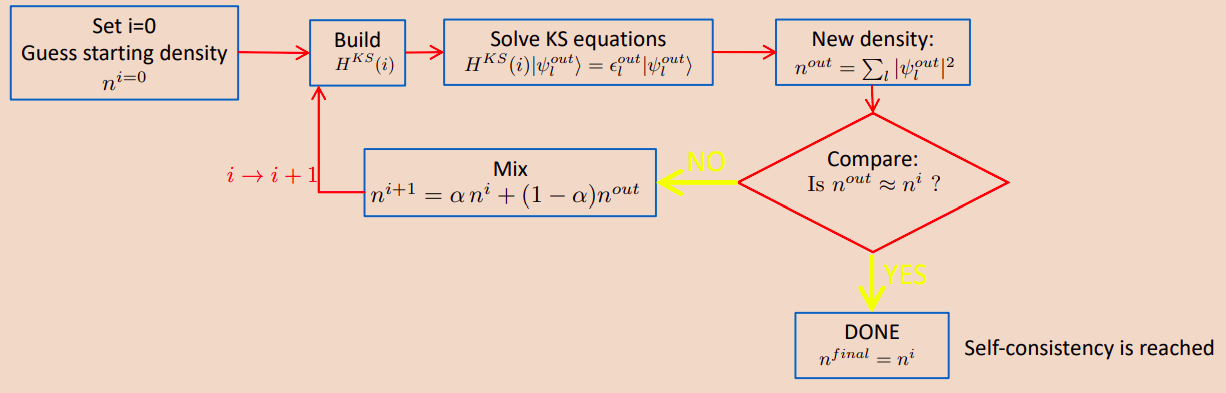
\includegraphics[scale = 0.4]{figs/D1/SCF.png}
      \caption{Esquema del ciclo autoconsistente.}
      \label{fig:SCF}
  \end{figure}

\subsection{PW como base del espacio de Hilbert}

  Dado que la computadora no puede almacenar funciones, sino que simplemente valores, necesitamos una base de funciones $\left\{ b_{\alpha} \right\}_{\alpha=1}^M$ a la cual asociarle dichos valores. A partir de esto definimos una cierta función $f$ como una CL de las funciones de la base según
    $$f (\vec{r}) = \sum_{\alpha = 1}^M c_{\alpha} b_{\alpha} (\vec{r})$$

  donde los coeficientes de la expansión $c_{\alpha}$ son los que se almacenan. El valor de $M$ debe ser lo suficientemente pequeño como para ahorrar memoria, pero lo suficientemente grande como para describir correctamente a $f$.

  El código a utilizar es representado en principio por la base que utiliza. En el caso de QE la base está construida por plane-waves (PW):
    $$b_{\alpha} (\vec{r}) = \frac{1}{\sqrt{V}} \exp{i \vec{G}_{\alpha} \cdot \vec{r}}$$

  \Obs{En QE básicamente todo está definido en términos de combinaciones lineales de senos y cosenos.}

  Los beneficios de utilizar PW como base son:
    \begin{itemize}
      \item Analíticamente simples, pudiendo derivar e integrar fácilmente.
      \item Ortonormales.
      \item No sesgadas: no asume la localización de las cargas ni de los electrones.
      \item Independientes de la posición de los núcleos: la base no va cambiando cuando se mueven los átomos (fuerzas de Pulay).
      \item Fácil control de la convergencia del tamaño de la base.
      \item Aplicación directa de FT, permitiendo aprovechar al máximo las dualidades entre el $R$- y el $G$-espacios.
    \end{itemize}

  Una de las principales desventajas es que el tamaño de la base suele ser mucho mayor que otras bases construidas por funciones localizadas, ya que no poseen información atómica.

\subsection{Periodicidad}

  Dada la naturaleza periódica de las PW, el uso de esta base está íntimamente relacionado con la periodicidad del sistema físico en estudio: son fácilmente aplicables a sistemas periódicos ya que basta definir la red de Bravais y su motivo.

  Si una función es periódica en el $R$-espacio, su FT es no nula únicamente para un conjunto infinito, pero discreto de vectores de onda.

\subsubsection{Caso 1D}

  En el caso de 1 dimensión, se tiene que
    $$\exp{i G_{\alpha}x} \rightarrow G_{\alpha} = n \frac{2\pi}{L} \quad n\in\mathbb{Z}$$

  donde $\sfrac{2\pi}{L}$ es la distancia entre las componentes no nulas de la FT, siendo $L$ el período (tamaño de las unidades que se repiten). A mayor $L$, mayor densidad de puntos no nulos en el $G$-espacio. La longitud de onda asociada a cierto vector de onda $\vec{G}_{\alpha}$ (Fig. \ref{fig:FT_1D}) cumple
    $$\lambda_{\alpha} \propto \frac{1}{\norm{\vec{G}_{\alpha}}}$$

  \begin{figure}[H]
      \centering
      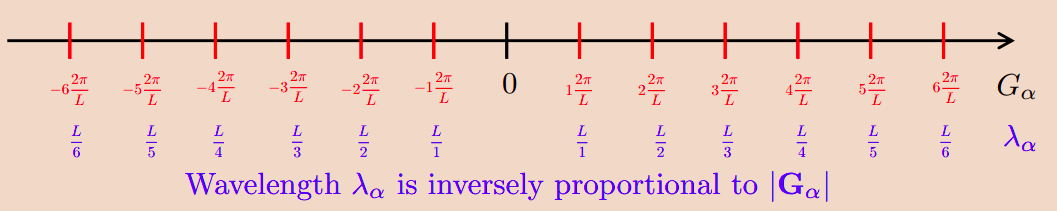
\includegraphics[scale = 0.4]{figs/D1/FT_1D.png}
      \caption{Representación de las infinitas componentes de Fourier en el $G$-espacio, denotando que son discretas. Se tienen además las longitudes de onda asociadas a cada vector de onda con componente no nula.}
      \label{fig:FT_1D}
  \end{figure}

  Aunque hemos logrado una discretización, para poder realizar un cálculo en la práctica necesitamos una cantidad finita de puntos. Para truncar la cantidad de puntos, uno determina una longitud de onda mínima $\lambda_{min}$, la cual sea suficiente para describir las características de interés (Fig. \ref{fig:FT_1D_min}).

  \Obs{Los orbitales y, por lo tanto, la densida de carga no varían en la escala de los núcleos atómicos, sino que varían en la escala de los \si{{\angstrom}}}.

  \begin{figure}[H]
      \centering
      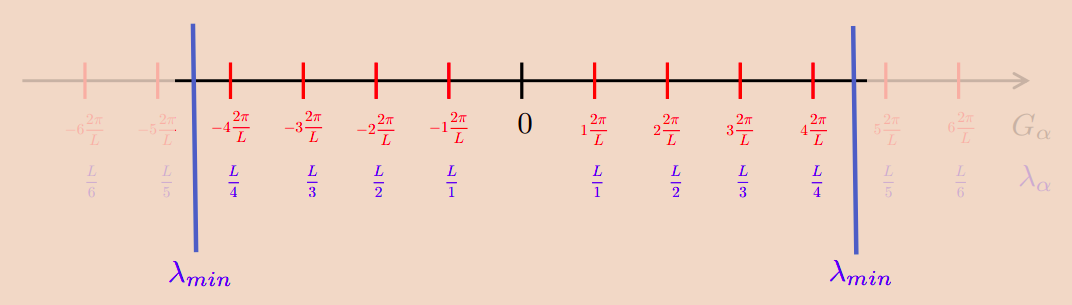
\includegraphics[scale = 0.4]{figs/D1/FT_1D_min.png}
      \caption{Truncamiento de las componentes no nulas en el $G$-espacio a partir de considerar cierto $\lambda_{min}$.}
      \label{fig:FT_1D_min}
  \end{figure}

  En la práctica uno no le dice al programa cuál es $\lambda_{min}$, sino que le indica la norma máxima para el vector de onda.
    $$G_{max} = \frac{2pi}{\lambda_{min}} \quad ; \quad G_{max} \equiv \norm{\vec{G}}_{max}$$

  En QE esto se hace estableciendo el cutoff de la energía cinética:
    $$E_{cut}^{\psi} = \frac{\hbar^2}{2m} G_{max}^2 \quad \equiv ecutwfc\ \ [Ry]$$

  \Obs{Este truncamiento es el que le indica a QE el tamaño de la base de PW. Como la ubicación de los puntos no nulos está directamente ligada al parámetro de red, se puede ver que la modificación de dicho parámetro altera la base de PWs utilizada: a mayor tamaño de red, la grilla de vectores $G$ se hace cada vez más densa y, manteniendo $G_{max}$ fijo, se irán agregando más PW al cálculo de manera discontinua. Esto se observa en una caída brusca en la enerǵia al agrandar el tamaño de la base. Si se presentan estas discontinuidades, hay que definir otras variables en el input: ecfixed, qcutz y q2sigma.}

\subsubsection{Caso 2D}

  Al considerar dos dimensiones, nuevamente tenemos el problema de que aunque son dicretos, tenemos infinitos puntos. En este caso, el truncamiento es una circunferencia (Fig. \ref{fig:FT_2D}). Se tiene
    $$\exp{i \vec{G}_{\alpha} \cdot \vec{r}} \rightarrow \vec{G}_{\alpha} = m \vec{B}_1 + n \vec{B}_2 \quad m,n\in\mathbb{Z}$$
  donde $\vec{B}_{1,2}$ son los vectores recíprocos de la red.

    \begin{figure}[H]
        \centering
        \subfigure[]{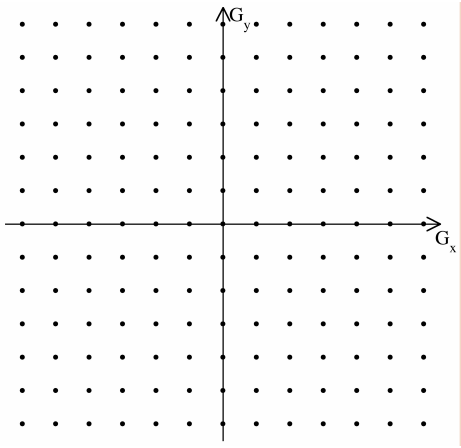
\includegraphics[scale = 0.3]{figs/D1/FT_2D_inf.png}}
        \subfigure[]{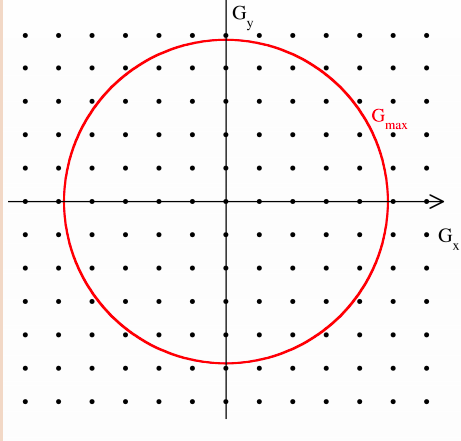
\includegraphics[scale = 0.3]{figs/D1/FT_2D_Gmax.png}}
        \subfigure[]{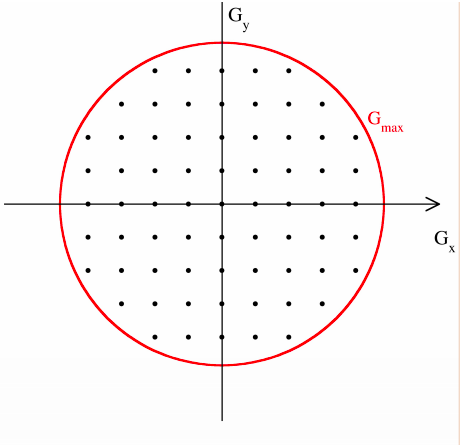
\includegraphics[scale = 0.3]{figs/D1/FT_2D_fin.png}} \\
        \caption{En el caso bidimensional el truncamiento se hace estableciendo una circunferencia de radio $G_{max}$.}
        \label{fig:FT_2D}
    \end{figure}

\subsubsection{Caso 3D}

  Extendiendo a 3 dimensiones:
    $$\exp{i \vec{G}_{\alpha} \cdot \vec{r}} \rightarrow \vec{G}_{\alpha} = m \vec{B}_1 + n \vec{B}_2 + p \vec{B}_3 \quad m,n,p\in\mathbb{Z}$$

  donde $\vec{B}_{1,2,3}$ son los vectores recíprocos de la red. Ahora el truncamiento es una esfera de radio $G_{max}$.

\subsection{Desde los orbitales KS hacia la densidad de carga}

  Considerando todo lo dicho, los orbitales KS expresados como CL de PWs con un cutoff $G_{max}$ son
    $$\psi_i (\vec{r}) = \sum_{\norm{\vec{G}} < G_{max}} c(\vec{G}) \exp{i \vec{G} \cdot \vec{r}}$$

  En el $R$-espacio dijimos que la densidad de carga viene dada por $n(\vec{r}) = \sum_{i=1}^N \psi_i^{*} (\vec{r}) \psi_i (\vec{r})$. Al convolucionar obtenemos la densidad de carga en el $G$-espacio:
    $$\tilde{n}(\vec{r}) = \sum_{i=1}^N \sum_{\norm{\vec{G}^{'}} < G_{max}} \tilde{\psi}_i^{*} (\vec{G}^{'}) \tilde{\psi}_i (\vec{G} - \vec{G}^{'})$$

  Al limitar $\norm{\vec{G}^{'}} < G_{max}$ estamos limitando las contribuciones de $\tilde{\psi}_i^{*} (\vec{G}^{'})$. Sin embargo, ahora la norma de $\vec{G}$ puede ser mayor que $G_{max}$ pues incluso cuando $\norm{\vec{G}} = 2 G_{max}$ y $\norm{\vec{G}^{'}} =  G_{max}$, se cumple que $\tilde{\psi}_i (\vec{G} - \vec{G}^{'}) \neq 0$.

  A partir de esto el análisis de Fourier nos dice que como la densidad de carga es un producto de 2 funciones truncadas según $G_{max}$, la densidad tendrá un cutoff mayor. Las componentes de Fourier no nulas estarán limitadas por $2G_{max}$. Este establece que en el cálculo tendremos dos bases: una para los orbitales, limitada por $G_{max}$, y una para la densdiad, conteniendo más puntos en el espacio recíproco ya que está limitada por $2G_{max}$. Esto lleva a la siguiente relación:
    $$E_{cut}^{n} \geq 4 E_{cut}^{\psi} \quad \equiv ecutrho\ \ [Ry]$$

  \Obs{Si no se hace esta distincción, se puede incurrir en aliasing errors. El código automáticamente establece la relación $ecutrho = 4 ecutwf$, teniendo que indicarla de manera explícita cuando necesitamos que un $ecutrho$ mayor.}

\subsection{Teorema de Bloch: primera zona de Brillouin}

  Aunque el sistema sea periódico, los orbitales no son necesariamente periódicos. En un sistema periódico, los orbitales de Bloch se relacionan con los orbitales KS según
    $$\psi_{\vec{k},i} (\vec{r}) = \exp{i \vec{k} \cdot \vec{r}} u_{\vec{k},i} (\vec{r})$$

  donde sólo la función $u_{\vec{k},i}$ es periódica ya que $\vec{k}$ no necesariamente es un punto de la grilla en el $G$-espacio, provocando que $\psi_{\vec{k},i}$ no sea periódica. Se tiene que
    $$u_{\vec{k},i} (\vec{r}) = \sum_{\norm{\vec{G}} < G_{max}} c_{\vec{k},i} \exp{i \vec{G} \cdot \vec{r}}$$

  la cual está definida sobre la grilla de $G$-vectores antes definida. Luego
    $$\psi_{\vec{k},i} (\vec{r}) = \sum_{\norm{\vec{G}} < G_{max}} c_{\vec{k},i} \exp{i \left(\vec{k} + \vec{G}\right) \cdot \vec{r}} $$

  obteniéndose una grilla corrida de $(k+G)$-vectores. A pesar del corrimiento, el cutoff no se ve alterado (Fig. \ref{fig:kg}).

    \begin{figure}[H]
        \centering
        \subfigure[]{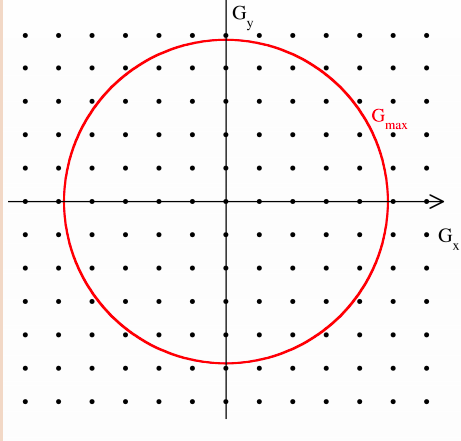
\includegraphics[scale = 0.3]{figs/D1/FT_2D_Gmax.png}}
        \subfigure[]{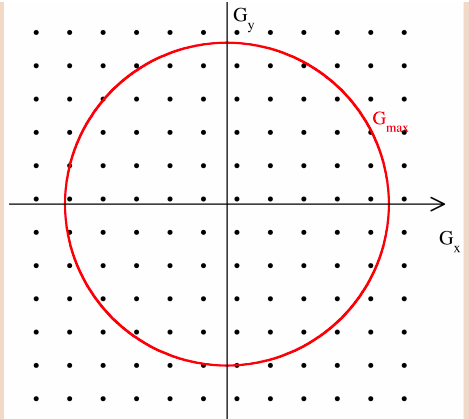
\includegraphics[scale = 0.3]{figs/D1/kg_1.png}} \\
        \subfigure[]{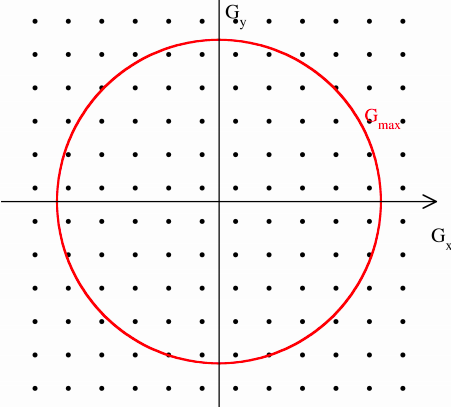
\includegraphics[scale = 0.3]{figs/D1/kg_2.png}}
        \subfigure[]{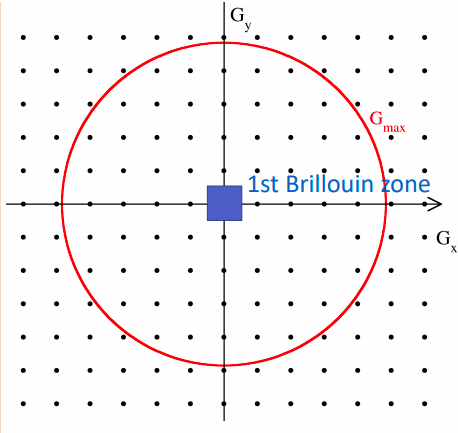
\includegraphics[scale = 0.3]{figs/D1/1BZ.png}} \\
        \caption{Grilla de $G$-vectores (a) comparada con dos posibles grilals de $(k+G)$-vectores, según dos posibles valores para $k$ (b y c). Se esquematiza además la 1BZ (d).}
        \label{fig:kg}
    \end{figure}

  Si al vector $\vec{k}$ se le suma un vector recíproco el resultado es indistinguible dada la periodicidad del sistema en el espacio recíproco. Esto lleva a que sólo sea necesario considerar la primera zona de Brillouin (1BZ): cualquier punto por fuera de la 1BZ será mapeado por el corrimiento a algún punto dentro de la 1BZ dada la periodicida. De este modo, aunque en un sistema periódico debemos sumar sobre todos los posibles valores de $k$-vectores, los únicos relevantes son aquellos que yacen dentro de la 1BZ. Luego, es importante hacer un buen muestreo de 1BZ.

  Supongamos que tenemos en 2 dimensiones una 1BZ rectangular cuyos vectores recíprocos son $\vec{B}_1$ y $\vec{B}_2$. Deseamos muestrear la 1BZ con una grilla de $k$-puntos de 4x4. Si la grilla es corrida en la mitad de la distancia que separa dos $k$-puntos consecutivos (Fig. \ref{fig:shift}), la convergencia será más rápida: dada la simetría que se genera, disminuyen la cantidad de cálculos que deben ser llevados a cabo. Sin embargo, en el caso no corrido, siempre tendremos presente el punto $k=0$ sin importar la simetría del sistema, pero se pierde al hacer el corrimiento.

  \Obs{En QE el corrimiento se hace cambiando los 0 por 1 en la carta de K\_POINTS automatic. Los cálculos con corrimiento no son comparables entre supercells (sistemas no 3D-periódicos) de tamaños diferentes por la pérdida de $k=0$. Generalmente conviene usar cuando tengo un sistema periódico que quiero que converja rápido.}

  \begin{figure}[H]
      \centering
      \subfigure[]{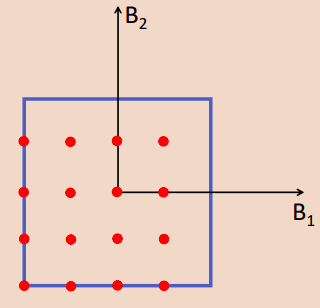
\includegraphics[scale = 0.4]{figs/D1/noshift.png}}
      \subfigure[]{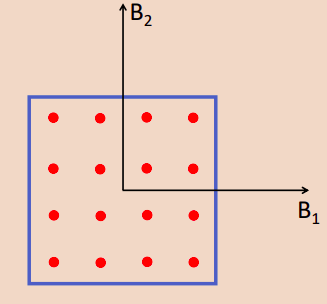
\includegraphics[scale = 0.4]{figs/D1/shift.png}} \\
      \caption{Muestreo de una 1BZ en 2 dimensiones con una grilla 4x4: original (a) y corrida (b).}
      \label{fig:shift}
  \end{figure}

\subsection{Sistemas no 3D-periódicos}

  Cuando se tiene un sistema que no es 3D-periódico, la solución es utilizar una supercelda: se agrega suficiente vacío en la celda como para que el sistema no vea a sus imágenes. Suficiente quiere decir tal que las interacciones entre ellas sean despreciables. De este modo evitamos interacciones espúreas.

  El problema de esto es cuando el sistema en estudio es cargado o dipolar: debido a la lentitud con la que decaen estas interacciones, deberíamos usar superceldas enormes. Para superar este problema existen dos soluciones:
    \begin{enumerate}
      \item Usar la variable assume\_isolated en el input, la cual es muy útil en sistemas 0D (moléculas, clusters, etcétera).
      \item Introducir una caoa dipolar en el vacío entre dos slabs consecutivos, utilizando la variable dipfield en el input.
    \end{enumerate}

\subsection{Pseudopotenciales}

  Si se considera la contribución radial de una función de onda para un cierto núcleo, se observa que en las cercanías del núcleo se presentan oscilaciones muy rápidas. Si quisiéramos muestrear esta primera región, necesitaríamos un $\lambda_{min}$ muy pequeño, lo que implicaría un cutoff muy grande para la energía cinética y, por lo tanto, una base de PWs mucho mayor (cálculo extremadamente caro). Sin embargo, en esta distancia no está la química pues es el core: todo ocurre a distancias mayores respecto al núcleo, donde la función ya es mucho más suave.

  El pseudopotencial da lugar a una pseudofunción de onda que tiene exactamente el mismo comportamiento que la función de onda original para todo radio mayor a cierto radio de corte ($r_{cut}$), pero que por debajo de dicho valor tiende suavemente a cero (Fig. \ref{fig:pseudo}). Esta pseudofunción de onda queda descripto por un $\lambda_{min}$ mayor, requieriéndose una base más pequeña, dando lugar a un cálculo más barato.

  \Obs{Los pseudopote afectan $V_{ext}$ en la ecuación KS.}

  \begin{figure}[H]
      \centering
      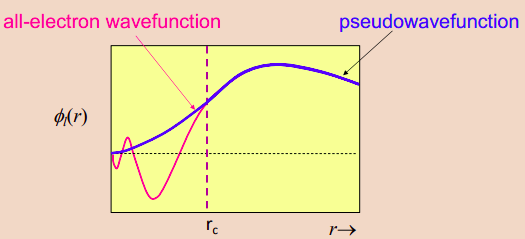
\includegraphics[scale = 0.6]{figs/D1/pseudo.png}
      \caption{Comparación de la función de onda original (all-electron) y la función de onda generada a partir del pseudopotencial.}
      \label{fig:pseudo}
  \end{figure}

  La condición necesaria para que el pseudopotencial sea transferible es que sea norm-conserving, \emph{i.e.} que la norma de ambas funciones sea la misma para valores por debajos del $r_{cut}$. De lo contrario, el átomo no tendrá las propieades de dispersión adecuadas.
    $$\int_0^{r_{cut}}\phi_{AE}^{*} (r) \phi_{AE} (r) dr = \int_0^{r_{cut}}\phi_{PS}^{*} (r) \phi_{PS} (r) dr$$

  \Obs{En la página materialsclouding.org/discover/sssp se tienen pseudopotenciales confiables.}

  Las características de un pseudopotencial son (Fig. \ref{fig:pseudoo}):
    \begin{itemize}
      \item Más débiles que un potencial coulómbico.
      \item No presentan singularidades en $r=0$.
      \item Iguales para $r$ grandes, pero dependientes del momento angular $l$ para $r$ pequeños.
    \end{itemize}

    \begin{figure}[H]
        \centering
        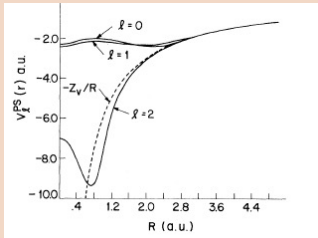
\includegraphics[scale = 0.6]{figs/D1/pseudoo.png}
        \caption{Comparación de un pseudopotencial con el potencial Coulómbico.}
        \label{fig:pseudoo}
    \end{figure}

  En QE los pseudopotenciales (PP) son provistos por el usuario en forma de archivos, que contienen la descripción del PP en una grilla radial. Los PP son específicos para cada elemento químico. Además, son dependientes del funcional utilizado: el código detecta automáticamente cuál fue el funcional utilizado y lo utilizará para resolver las ecuaciones KS. En este sentido, es conveniente que todos los PP que se usan en una misma corrida hayan sido creados considerando el mismo funcional.

\subsubsection{Problemas con la conservación de la norma}

  Existen ciertos elementos para los cuales la condición de conservación de la norma termina siendo un problema: se dan cutoffs mayores de lo que uno querría. Esto ocurre especialmente cuando la función de onda no tiene nodos.

  En estos casos uno puede remover la condición de conservación de norma. Sin embargo, para que los resultados sean confiables, debemos recurrir a una expresión más complicada para la densidad de carga electrónicas
    $$n (\vec{r}) = \sum_{i=1}^N \psi_i^{*} (\vec{r}) \psi_i (\vec{r}) + n^{aug} (\vec{r})$$

  donde el término $n^{aug}$ es la augmentation charge density, la cual está localizada en torno al núcleo y da cuenta de la norma que se estaba perdiendo, expresada en términos de proyectores.

  Este es el caso de los ultrasoft PP (USPP) y los PAW PP. Tenemos entonces que, a pesar de que la norma no se conserva mediante la misma condición de antes, logramos alcanzar la misma norma al sumarle este nuevo término. Las consecuencia de esto es que necesitamos cutoff mayores ($E_{cut}^{n} > 4 E_{cut}^{\psi}$) y, por lo tanto, debemos darle a QE ambos valores necesariamente: tanto ecutwfc como ecutrho. Esto lleva a que haya que chequear la convergencia de ambos parámetros.

\section{Q\&A}

  \definicion{What is the reason for the weight $\alpha$ for the density? Why not just take n\_out in the scf cycle?}

  The mixing parameter (not weight!) $\alpha$ is important for the SCF cycle to converge. If you simply take n\_out, then is is very likely that you only oscillate between various densities. The mixing (which is in reallity more sophisticated that what I have shown in the slides) akts like a friction term. You add only a (normally small) piece of the new density, guaranteeing that step by step you approach the self-consistent solution

  \definicion{what is the convergency criterion? what does the total scf accuracy in every iteration measure? the difference between the current and previous total energy?}

  What the code prints as "scf accuracy" is in fact an energy: it first calculates the difference of the density between "in" and "out", and then estimates an energy by plugging this "$\delta$ rho" into the formula for a Hartree energy. It is in a sense the classical Coulomb interaction energy of the change in density. As "$\delta$\_rho" goes to zero, so does this quantity. Reference: function rho\_ddot in scf\_mod.f90

  \definicion{Do we also check the density separately? How is the convergence checked?}

  The convergence is checked by this quantity (called dr2 in the code). It is not a change in estimated total energy, but a measure of the norm of the change in charge density

  \definicion{US and PAW, what should one chose and when? This ties maybe to a deeper question about how much should the final user care about their choice of PP. To what extent are the PP influencing the results? how realistic is a scenario where I completely have to throw away work because of the wrong choice of pseudopotential? What are the main pitfalls to avoid? Does this availability of multiple pseudos influence reproducibility?}

  From a user's perspective, the choice of either US or PAW is only relevant if you plan to do calculations  where you need to obtain the additional info which PAW can provide you: in PAW you can "reconstruct" the shape of the all-electron wavefunctions close to the nucleus. This info in needed for certain properties, for example if you are interested in NMR chemical shifts. If you are not interested in such (very particular) applications, then you can use US and PAW both in the same way.

  About pseudopotentials in general: in the past, this was a huge issue: many old calculations you find today in the literature are in fact wrong - because of wrong pseudopotentials. Either the potentials were outright wrong, or (more common) people used pseudopotentials where some semi-core electrons were "hidden" in the core, while it would have been important to include them in the (explicitly treated) valence. Today, one knows about the importance of such "semi-core" electrons, and pays more attention.

  As a user, make sure that you do not blindly download PPs from some obscure (and perhaps old) database, where you do not know if the PPs have been checked and controlled carefully. One very exemplary source for PPs (limited to PBE and PBEsol functionals) is this one: https://www.materialscloud.org/discover/sssp/table/efficiency Here, they have made a very thorough and exemplary job of checking everything against all-electron calculations. But also the pslibrary are generally reliable https://www.quantum-espresso.org/pseudopotentials

  As a user, still in every case, check which is the valence configuration for every pseudopotential ("how many electrons are in the valence?") and in case of doubt, compare with another pseudopotential which contains more electrons

  \definicion{I'm confused about the mixing number alpha and beta, since the mixing\_beta is what I include in calculations and I thought this was the mixing parameter responsible of combining old and new densities. Am I mistaken?}

  Sure, this was my fault. What I called $\alpha$ in my talk is called $\beta$ in pwscf ...

  \definicion{In the lecture, there was this dipfield tag recommended for 2D systems. Would that apply to graphene? Could you please comment further on that tag?}

  No need for that in the case of pristine graphene as it does not have the electrostatic dipole moment. The dipole layer correction should be applied only in cases when you have a 2D material (which lies in x0y plane) that is an insulator and has considerable dipole moment pointed in the z-direction. In such cases the electrostatic potential is not the same on both sides of 2D material, thus the dipole layer correction should be applied. Usually you apply it when you want to calculate the work function.

  \definicion{If I doing scf calculation i don’t know how me bands looks like. How do I know that I have insulated system or the system have dipole moment?}

  Best way: plot density of states with dos.x after you do scf and nscf. I recommend this.

  Quickest way: in the \&CONTROL flag of the pw.graphene.scf.in set the verbosity='high' and do the calculation with smearing turned on. Then in the output file you will get the occupation numbers for all the k-points. If some of them are fractional numbers then you got a metal.

  NB. In case of graphene, when you do not have included the special point K in the k-point grid and you have very small smearing you will falsely get a narrow gap semiconductor (the gap is decreasing with the number of k-points but will never go away unless you include point K or increase the smearing).

  \definicion{When I have to use vdw corretion (vdw\_corr) in scf calculation?}

  You use vdw\_corr when you have two subsystems A and B that are interacting very weakly, usually by means of dipol-(induced) dipol interaction. Those kind of interactions are called van der Waals interactions. For instance, when you adsorb graphene on top of Ni(111) and you want to calculate adsorption energy with PBE functional, if you do not put vdw\_corr you won't be able to obtain the adsorption energy, it will be basically zero.

  Or even simpler example - you have bilayer graphene and you use PBE functional to obtain the interaction (adhesion) energy between two sheets. If you plot E\_adh vs distance you will see that there is no minimum. On the other hand, if you put vdw\_corr you will clearly see the minimum at some distance between 2 and 3 angstroms

  \definicion{In the second example from today, why do the number of k-points change from the scf to the nscf calculation? (from 9 9 1 to 12 12 1)}

  because we compute the DOS with the tethraedra method that need a denser mesh

  it is not so crucial as in the scf case, in particulare for DOS and pDOS is more about about the quality of the plot, but in principle yes one should check whether denser mesh change the result significantly

  \definicion{What are the main reasons for choosing one Pseudopotential over another?}

  1. accuracy ; 2. economy; 3. a tradeoff between 1 and 2

  \definicion{I have a qustion regarding k-grid. As this parameter is a consequence of periodicity - what do I do with amorphous cell? Gamma-only because of no long-range order or test k-grids?}

  A test is necessary... Even if you think that the system is “aperiodic”, for the electrons it is not. If you have a small cell, your electrons will “see” the periodicity, and thus there is band dispersion, and thus sampling of the Brillouin zone is needed. If you have a large cell, the periodicity through the cell is no longer “seen” by the electrons, and Gamma-only is sufficient. Your system is probably between these two extrema, very small and extensively large, and thus, depending on the size and type of electronic structure, you might be forced to test for the convergence indeed.

  PS: for a disordered system, you can think of k-point sampling as of a sampling over boundary conditions for the wavefunctions. At k=0, wavefunctions are periodic over the simulation cell. At zone border, they are antiperiodic, etc. As the choice of boundary conditions is to a large extent a matter of convention, it makes sense to sample different choices for them. For large enough systems, calculated properties are independent of the boundary conditions, and sampling just the Gamma point would do.

  \definicion{how do I choose an appropriate mixing\_beta parameter for each system?}

  You start from the default value. Which is 0.7. In most cases this is ok. If the scf cycle does not converge, then use a smaller value. Sometimes as small as 0.1 is needed. However, if you encounter serious convergence problems in the scf cycle, then often it helps to introduce some smearing with finite temperature. This avoids that some states discontinuously cross the Fermi level and are therefore occupied/empty in subsequent iterations. Very often, smearing helps more to make your cycle converge than changing mixing\_beta

  \definicion{¿Podría correr con shift en los k-points  para hacer una relajación y, una vez que esté relajado, seguir los cálculos sin el corrimiento?}

\section{Hands-on}

    \definicion{Topic:} How to compile Quantum ESPRESSO. SCF calculations + post-processing – part 1. XCrySDen, PWgui, QE-emacs-modes, and PWTK

    \definicion{Speaker:}	Pietro DELUGAS (SISSA, Italy).

\subsection{Benzene}

\subsubsection{Objetivo} Aprender a calcular y plotear orbitales moleculares en benceno.

\subsubsection{Pasos}
    \begin{enumerate}
      \item Hacer un cálculo SCF (pw.x) para determinar los estados KS.
        \begin{verbatim}
          pw.x < pw.benzene.scf.in > pw.benzene.scf.out
        \end{verbatim}
      \item Calcular todos los MO de valencia y el LUMO (pp.x) según $sign(\psi (\vec{r})) \norm{\psi (\vec{r})}^2$. Los resultados se escriben en un archivo psi2.benzene\_K001\_B0*.xsf.
        \begin{verbatim}
          pp.x < pp.benzene.psi2.in > pp.benzene.psi2.out
        \end{verbatim}
      \item Graficar uno de los archivos XSF generados con xcrysden. Por ejemplo
        \begin{verbatim}
          xcrysden --xsf psi2.benzene_K001_B006.xsf
        \end{verbatim}

            Luego, mejorar la calidad de la gráfica y guardar el estado (File-->Save Current State). Supongamos que el estado fue guardado como MO-state.xcrysden, luego el estado puede levantarse con otro orbital haciendo
        \begin{verbatim}
          xcrysden --xsf psi2.benzene_K001_B005.xsf --script MO-state.xcrysden
        \end{verbatim}
      \item Para graficar todos los MO ejecutar en la terminal
        \begin{verbatim}
          ./plot-psi2.sh
        \end{verbatim}
    \end{enumerate}

\subsubsection{Resultados}

  En los inputs, QE toma como comentarios a aquellas líneas que comienzan con ! o con \#. Si no se escriben los valores para $pseudo\_dir$ y $outdir$, pw.x va a recurrir a los variables de ambiente: ESPRESSO\_PSEUDO y ESPRESSO\_TMPDIR, respectivamente (esto lo definimos en el .bashrc).

  En la carpeta de archivos temporales se genera, por cada prefix, una carpeta (prefix.save/) y un archivo XML (prefix.xml): la carpeta contiene binarios para hacer procesamientos posteriores, mientras que en el xml se tiene información general acerca de la corrida.

  Para los cálculos se utilizaron USPP con PBE como funcional:
    \begin{itemize}
      \item C.pbe-rrkjus.UPF
      \item H.pbe-rrkjus.UPF
    \end{itemize}

  Se puede usar emcas para que reconozca las variables relevantes del QE, sino se pueden crear unos archivos que permiten que vim las detecte (https://github.com/leseixas/quantum\_espresso-vim).

  Se conocen como namelists a aquellos bloques que comienzan con \&, mientras que los demás bloques se denominan cards.

  Para correr sobre M procesadores (teniendo mpi):
    \begin{verbatim}
      mpirun -np M pw.x -i input\_file.in > output\_file.out
    \end{verbatim}

  Si escribimos
    \begin{verbatim}
      mpirun -np M pw.x -i input\_file.in | tee output\_file.out
    \end{verbatim}

  nos irá mostrando el cálculo en pantalla además de guardarl en el archivo de destino.

  En pp.x dentro del namelist \&INPUTPP las variabes kband(1) y kband(2) le indican desde y hasta qué orbital queremos calcular, respectivamente. En este caso queremos los 16 orbitales. Además lsign le pide que conserve el signo de la función cuando es .true.

  Luego en la namelist \&PLOT tenemos:
    \begin{itemize}
      \item \textbf{iflag:} como es 3 le estamos pidiendo que grafique en 3 dimensiones.
      \item \textbf{nfile:} le indica que sólo debe considerar un archivo.
      \item \textbf{weight(1):} en este caso sólo hay un archivo (nfile=1) y por eso se le pone peso 1. Sin embargo, podría tener más de un archivo que considerar y con esta variable puedeo ponderar dicha consideración.
    \end{itemize}

  Al correr pp.x se van a generar 2 arhivos por orbital: uno propio de QE y otra para que pueda ser levantado por xcrysden.

  Para que xcrysden considere la información del orbital, debemos ir a $Tools > Datagrid$ y seleccionar lo que deseamos graficar (en este caso sólo habrá una opción disponible ya marcada dentro de la gráfica de árbol). El mutiply factor es la densidad de carga dividido el volumen de la celda. Al estar usando una molécula asilada, la celda es mucho mayor que la densidad de carga. Luego debemos usar un valor grande: usaremos 100.

  Al dar $ok$ se abre un nuevo menú. Lo que nos interesa es ingresar un isovalor para la densidad de carga electrónica (cuadrado rosa vacío). Este valor debe encontrarse entre los extremos que están por encima de este cuadrado y en grisesito. Esto permitirá que se genere una isosuperficie. Conviene tildar $Render +/- isovalue$ para detectar las zonas con densidad de carga de diferente signo. Al poner $Submit$ vemos que sobre la molécula se grafican los orbitales.

  \Obs{No hay una regla para elegir el isovalor. Debe ser uno tal que permita observar claramente todas las características de lo que queremos mostrar. Si vamos a comparar entre varias isosuperficies, hay que chequear que todas queden bien presentadas para su análisis utilizando el mismo isovalor. Valores más cercanos a 0 tienden a mostrar isosuperficies más grandes, tendiendo a perderse un poco la cuestión.}

  \begin{figure}[H]
      \centering
      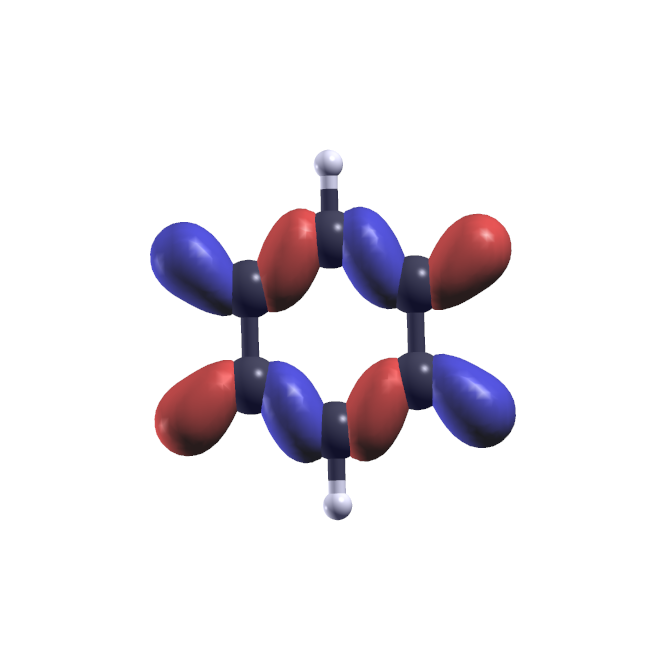
\includegraphics[scale = 0.4]{figs/D1/psi2.benzene.png}
      \caption{Doceavo MO para el benceno.}
  \end{figure}

\subsection{Graphene}

\subsubsection{Objetivo}

  Calcular y plotear DOS y estructura de bandas (spaghetti) de una hoja de grafeno.

\subsubsection{Pasos}

    \begin{enumerate}
      \item Hacer un cálculo SCF (pw.x) para determinar los estados KS.
        \begin{verbatim}
          pw.x < pw.graphene.scf.in > pw.graphene.scf.out
        \end{verbatim}

      \item Plotear DOS:
        \begin{enumerate}
          \item Hacer un cálculo no SCF (pw.x) con una grilla más densa de puntos k (aumenta la \emph{definición} de la DOS).
            \begin{verbatim}
              pw.x < pw.graphene.nscf.in > pw.graphene.nscf.out
            \end{verbatim}
        \item Hacer el cálculo para genera el datafile de la DOS (dos.x). El resultado se escribe en el archivo graphene.dos.
          \begin{verbatim}
            dos.x < dos.graphene.in > dos.graphene.out
          \end{verbatim}
        \item Plotear la DOS con gnuplot.
          \begin{verbatim}
            gnuplot dos.gp
          \end{verbatim}
        \end{enumerate}

      \item Plotear estructura de bandas:
        \begin{enumerate}
          \item Hacer un cálculo de bandas ($calculation = 'bands'$ en pw.x) para determinar los autovalores sobre los puntos k a lo largo de cierto camino.
            \begin{verbatim}
              pw.x < pw.graphene.bands.in > pw.graphene.bands.out
            \end{verbatim}
          \item Hacer un cálculo para generar un archivo fácil de plotear (bands.x). El resultado se escribe en el archivo graphene.bands.dat.gnu.
            \begin{verbatim}
              bands.x < bands.graphene.in > bands.graphene.out
            \end{verbatim}
          \item Plotear el spaghetti con gnuplot.
            \begin{verbatim}
              gnuplot spaghetti.gp
            \end{verbatim}
        \end{enumerate}
      \item Colocar el valor correcto de la energía de Fermi en los gnuplot files.
        \begin{enumerate}
          \item Encontrar la energía de Fermi en el output (pw.graphene.nscf.out).
          \begin{verbatim}
            grep Fermi pw.graphene.nscf.out
          \end{verbatim}
          \item Editar los archivos dos.gp y spaghetti.gp con el valor hallado. Descomentar la línea $set yzeroaxis lt -1$
          \item Replotear ambas gráficas.
          \begin{verbatim}
            gnuplot dos.gp
            gnuplot spaghetti.gp
          \end{verbatim}
        \end{enumerate}
    \end{enumerate}

\subsubsection{Resultados}

  Para los cálculos se utilizaron USPP con PBE como funcional (el mismo que usamos en el benceno): C.pbe-rrkjus.UPF


  Las diferencias entre los inputs para el SCF y el non-SCF son:
    \begin{itemize}
      \item \textbf{calculation:} $'scf' \Rightarrow'nscf'$
      \item \textbf{k-mesh grid:} $9\ 9\ 1 \Rightarrow 12\ 12\ 1$
      \item \textbf{occupations:} $vacio \Rightarrow 'tetrahedra_opt'$
      \item \textbf{:} $ \Rightarrow $
    \end{itemize}

  Como queremos calcular la DOS, necesitamos una malla más densa de puntos para tener más detalle de lo que está pasando. Básicamente hacemos que el cálculo sea más fino.

  En el archivo graphene.dos encontramos tanto la enería de Fermi como la DoS y la DoS integrada.

  \begin{figure}[H]
      \centering
      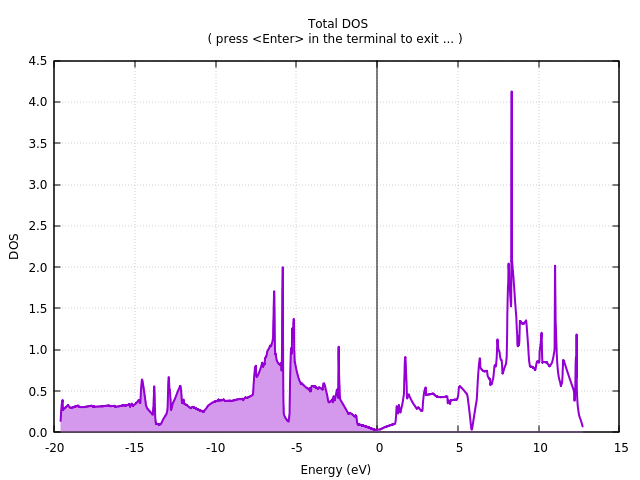
\includegraphics[scale = 0.6]{figs/D1/dos.png}
      \caption{DoS para la capa de grafeno: la zona sombreada representa ocupación electrónica, llegando hasta la energía de Fermi (línea negra).}
  \end{figure}

  Cuando hacemos el cálculo de las bandas, debemos pedir $calculation = 'bands'$ y con $nbnd$ especificamos el número de bandas: por default el programa sólo graficará las ocupadas, por lo que debemos poner un número mayor para observar bandas desocupadas. Otra diferencia es que le ponemos el camino de puntos K que queremos que siga.

  \begin{figure}[H]
      \centering
      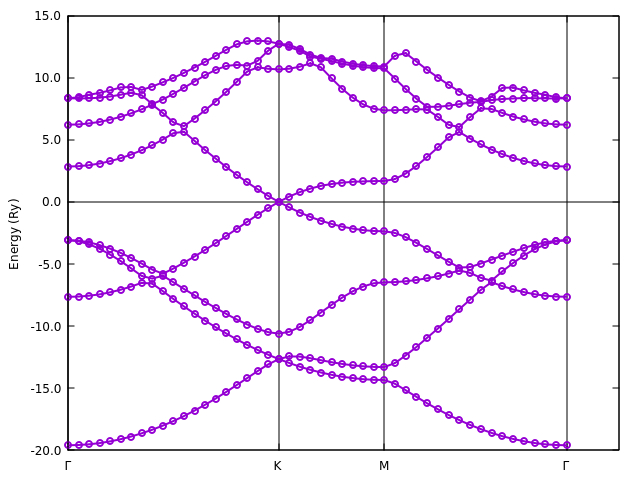
\includegraphics[scale = 0.6]{figs/D1/bandas.png}
      \caption{Estructura de bandas para el grafeno. Se observa el punto de Dirac al valor de la energía de Fermi.}
  \end{figure}

  Para seleccionar el camino de puntos k, podemos usar xcrysden. Para ello debemos ir a $Tools > k-path\ selection$ y esto nos permitirá seleccionar interactivamente el camino deseado.


    \chapter{Día 2}

      \section{Teórico}

  \definicion{Topic:} Charge densities and potentials. Systems in 0-1-2-3D. Metals vs. insulators. Non-magnetic vs. magnetic systems.

  \definicion{Speaker:} Paolo GIANNOZZI (University of Udine, Italy)

\subsection{DFT}

  Dada una función unidimensional $L$-periódica $f$, la transformada de Fourier (FT) nos permite establecer que
    $$f(x) = \sum_n \tilde{f} (q_n) e^{iq_n x} \quad ; \quad \tilde{f} (q_n) = \frac{1}{L} \int f(x) e^{-iq_n x} dx$$

  donde
    $$q_n = n \frac{2\pi}{L} \quad ; \quad n \in \mathbb{Z}$$

  En el caso de la transformada de Fourier discreta (DFT) se considera un conjunto finito de valores, tanto para $q$ como para $x$, volviéndose ambas variables periódicas: los valores negativos son mapeados al correspondiente positivo.
    $$f(x) \rightarrow f_m \equiv f(x_m) \quad ; \quad x_m = m \frac{L}{N} \quad ; \quad m \in [0, N-1]$$
    $$\tilde{f}(q) \rightarrow \tilde{f}_n \equiv \tilde{f}(q_n) \quad ; \quad q_n = n \frac{2\pi}{L} \quad ; \quad n \in [0, N-1]$$

  El valor de $N$ tiene que ser lo suficientemente grande como para incluir correctamente todas las componentes de Fourier en el $q$-espacio.

  Reuniendo todo esto, la DFT se escribe como
    $$f_m = \sum_{n=0}^{N-1} \tilde{f}_n e^{i2\pi \frac{nm}{N}} \quad ; \quad x\text{-espacio}
    \quad\quad\quad\quad
    \tilde{f}_n = \sum_{m=0}^{N-1} f_m e^{-i2\pi \frac{nm}{N}} \quad ; \quad q\text{-espacio}$$

  Para extender esto a 3 dimensiones, consideramos primero un conjunto de vectores de la red recíproca $\vec{G}$ centrados en el origen, dados por
    $$\vec{G} = n_1^{'} \vec{G}_1 + n_2^{'} \vec{G}_2 + n_3^{'} \vec{G}_3$$

  siendo $\vec{G}_{1,2,3}$ los vectores primitivos. La grilla sobre el $G$-espacio es periódica por construcción. Análogamente en el $R$-espacio se tiene que
    $$\vec{r} = \frac{m_1}{N_1} \vec{R}_1 + \frac{m_2}{N_2} \vec{R}_2 + \frac{m_3}{N_3} \vec{R}_3 \quad ; \quad m_s\in[0, N_s - 1]$$

  siendo $\vec{R}_{1,2,3}$ los generadores de la red de Bravais. En el caso 3D también debemos tomar un conjunto finito. Para ello
    $$f(\vec{r}) = \sum_G \tilde{f} (\vec{G}) e^{i \vec{G}\cdot\vec{r}} \rightarrow f(m_1, m_2, m_3)
    \quad\quad\quad\quad
    \tilde{f}(\vec{G}) = \frac{1}{\Omega} \int f (\vec{r}) e^{-i \vec{G}\cdot\vec{r}} d \vec{r} \rightarrow \tilde{f}(n_1, n_2, n_3)$$
    $$f(m_1, m_2, m_3) = \sum_{n_1, n_2, n_3} \tilde{f} (n_1, n_2, n_3) \prod_j e^{i 2 \pi \frac{n_j m_j}{N_j}}$$
    $$\tilde{f}(n_1, n_2, n_3) \frac{1}{N} \sum_{m_1, m_2, m_3} f (m_1, m_2, m_3) \prod_j e^{-i 2 \pi \frac{n_j m_j}{N_j}}$$

  donde $N = N_1 N_2 N_3$ y $\vec{G}_i \cdot \vec{R}_j = 2\pi\delta_{ij}$.

\subsection{DFT y orbitales KS}

  Ya vimos que
    $$\psi_i (\vec{r}) = \frac{1}{V} \sum_G c_{\vec{k} + \vec{G}} \exp{i (\vec{k} + \vec{G}) \cdot \vec{r}}
    \quad ; \quad
    \frac{\hbar^2}{2m} \norm{\vec{k} + \vec{G}}^2 \leq E_{cut}$$

  La densidad de carga es entonces
    $$n (\vec{G}^{'}) = \sum_G \sum_{i,k} f_{i,k} c_{i,\vec{k} + \vec{G}}^{*} c_{i,\vec{k} + \vec{G} + \vec{G}^{'}}$$

  con lo que aparecen componentes $\vec{G}^{'}$ tales que $max\left(\norm{\vec{G}^{'}}\right) = 2 max\left(\norm{\vec{G}}\right)$.

  Esto lleva a que sea necesario el cutoff de la energía cinética para las componentes de Fourier, tanto en la densidad de carga como en los potenciales, sean al menos 4 veces mayores que el cutoff de a base de PWs.
    $$\frac{\hbar^2}{2m} \norm{\vec{G}}^2 \leq 4 E_{cut}$$

  Esta inecuación es la que nos indica qué tan grande debe ser la grilla: debe ser suficiente para incluir todos los $G$-vectores hasta satisfacerla. Generalmente la grilla incluye también componentes de Fourier que no son útiles (más allá del cutoff recién dicho).

  \begin{figure}[H]
      \centering
      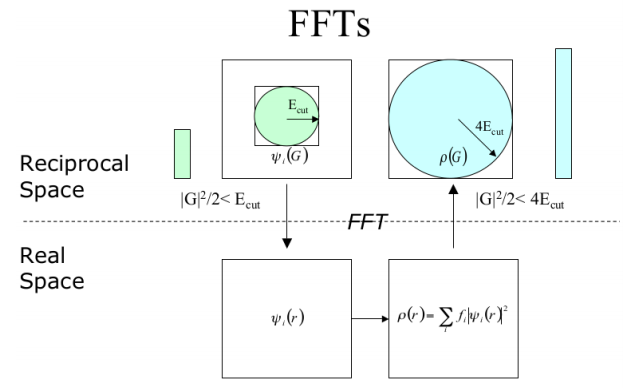
\includegraphics[scale = 0.6]{figs/D2/FFT.png}
      \caption{El cuadrado representa la caja (grilla) sobre la que se efectúa la FT. Para los orbitales KS sólo se requiere $\sfrac{1}{8}$ de la misma (izquierda), mientras que para la densidad de carga requiero  ocupar todavía más.}
      \label{fig:FFT}
  \end{figure}

\subsection{FFT}

  Mientras que el costo computacional de la FT convencional para $n$ partículas es tal que $t_{CPU} = \mathcal{O} (n^2)$, el costo para la transformada rápida de Fourier (FFT) va como $t_{CPU} = \mathcal{O} (n \log{n})$. Esto da lugar a una enorme mejora el los cálculos PW.

\subsection{Dual space technique}

  Teniendo
    $$H\psi = (T + V_{NonLoc} + V_{loc} + V_H + V_{xc})\psi$$

  se cumple que
    \begin{itemize}
      \item $T\psi$ es más fáci de clacularen el $G$-espacio: $t_{CPU} = \mathcal{O} (n)$
      \item $(V_{loc} + V_H + V_{xc})\psi$ es más fácil de calcular en el $R$-espacio: $t_{CPU} = \mathcal{O} (n)$
      \item $V_{NonLoc}\psi$ es fácil en ambos espacios siempre que el operador sea separable en proyectores: $t_{CPU} = \mathcal{O} (mn)$ siendo $m$ la cantidad de proyectores utilizados.
    \end{itemize}

  Con esto en mente, se utiliza la FFT para ir y volver entre el $R$-espacio y el $G$-espacio a conveniencia.

\subsection{Simetrización de la densidad de carga}

  La densidad de carga calculada por el código está no simetrizada:
    $$\tilde{n} (\vec{r}) = \sum_{k\in IBZ} \sum_v \omega_k \norm{\psi_{k,v} (\vec{r})}$$

  donde la suma corre sólo sobre estados ocupados y $k$-puntos simétricamente inequivalentes, los cuales pertenecen a la zona de Brillouin irreducible (IBZ), la cual es la 1BZ reducida por todas las operaciones de simetría del grupo puntual al que pertenece el cristal. Los coeficientes $\omega_k$ pesan la simetría: es la cantidad de $k$-puntos que son equivalentes a $k$ por simetría.

  \Obs{Tanto la grilla de $k$-puntos sobre la IBZ como los $\omega_k$ pueden ser calculados o provistos por el usuario.}

  La verdadera densidad de carga se obtiene via simetrización:
    $$n(\vec{r}) = \frac{1}{N_S} \sum_{n=1}^{N_S} \hat{O}_n \tilde{n} (\vec{r}) = \frac{1}{N_S} \sum_{n=1}^{N_S}  \tilde{n} (O_n^{-1} \vec{r})$$

  donde $\hat{O}_n$ es la $n$-ésima simetría del cristal y $O_n$ es la matriz de rotación asociada. Para grupos que contienen operaciones de simetría con traslaciones fraccionarias, lo anterior se generaliza a
    $$n(\vec{r}) = \frac{1}{N_S} \sum_{n=1}^{N_S}  \tilde{n} (O_n^{-1} \vec{r} - \vec{f}_n)$$

  siendo $\vec{f}_n$ la traslación fraccionaria con respecto al vector de red para la $n$-ésima operación.

  \Obs{En pw la simetrización es llevada a cabo en el $G$-espacio por lo que
    $$n(\vec{G}) = \frac{1}{N_S} \sum_{n=1}^{N_S}  \tilde{n} (O_n^{-1} \vec{G}) \exp{-i O_n^{-1} \vec{G}\cdot\vec{f}_n)}$$}

\subsection{Augmentation charge}

  Para USPP y PAW PP se agrega el término de augmentation charge. Así
    $$n^{aug} (\vec{r}) = \sum_{\mu,l,m} \braket{\psi_i}{\beta_l} Q_{\mu,l,m} (\vec{r}) \braket{\beta_m}{\psi_i}$$

  donde $\mu$ corre sobre los núcleos mientras que $\beta_l$ y $Q_{\mu,l,m}$ son funciones de corto alcance centradas en el átomo $\mu$.

  El primer término de $n (\vec{r})$, dado por $\norm{\psi_i (\vec{r})}^2$, se calcula fácilmente con la misma grilla de FFT utilizada en el cálculo de $H\psi$, conteniendo las componentes de Fourier del $G$-espacio hasta la energía cinética de $4E_{cut}$. El término de augmentation charge se calcula en una grillas más grande y densa, conteniendo $G$ hasta un cutoff mayor que $4E_{cut}$.

\subsection{Metales}

\subsubsection{Densidad de carga en metales}

  La manera más directa de calcular con metales es introducir un ensanchamiento de los niveles discretos. Así
    $$n(\vec{r}) = \sum_i f_i \norm{\psi_i (\vec{r})}^2 $$

  donde $f_i\in [0,1]$ son ocupaciones fraccionaraias dadas por
    $$f_i = \int_{\epsilon < \epsilon_F} \delta (\epsilon - \epsilon_i) d \epsilon \quad ; \quad \sum_i f_i = N_{\epsilon_F}$$

  y la energía de Fermi $\epsilon_F$ queda determianda por la condición $N_{\epsilon_F}  = N_{elec}$. El integrando $\delta(x)$ es la función (normalizada) de ensanchamiento. Aunque uno podría utilizar la función de Fermi-Dirac en principio, no es conveniente ya que se necesitaría una temperatura muy alta y la distribución tendría colas muy largas.
    $$\delta_{FD} (x) = \frac{1}{e^{x\beta} + 1}$$

\subsubsection{Energía en metales}

  La manera de calcular la energía es
    $$E_{KS} = \sum_i \int_{\epsilon < \epsilon_F} \epsilon \delta (\epsilon - \epsilon_i) d \epsilon = \tilde{E}_{KS} + \delta E_{met}$$

  donde
    $$\tilde{E}_{KS} = \sum_i \epsilon_i \int_{\epsilon < \epsilon_F}  \delta (\epsilon - \epsilon_i) d \epsilon = \sum_i f_i \epsilon_i
    \quad ; \quad
    \delta E_{met} = \sum_i \int_{\epsilon < \epsilon_F} (\epsilon - \epsilon_i) \delta (\epsilon - \epsilon_i) d \epsilon$$

  Esta contribución $\delta E_{met}$ aparece en el output como $smearin\ contrib.\ (-TS)\ \ [Ry]$.

\subsubsection{Funciones de ensanchamiento}

  Una posibilidad es la función Gaussiana normalizada
    $$\delta(x) = \frac{1}{\sigma \sqrt(\pi)} e^{-\frac{x^2}{\sigma^2}} \quad ; \quad \int \delta(x) = 1$$

  donde $\sigma$ (medido en Ry y escrito como $degauss$ en el input) da lugar a una temperatura ficticia $T=\sfrac{\sigma}{k_B}$ a la cual se corresponde un funcional de energía libre $E_{KS} [\sigma]$.

  Se puede ver que $E_{KS} [\sigma] \propto \sigma^2$ por lo que a mayor $\sigma$ (lo cual hace falta para una convergencia rápida de $k$-puntos) dan lugar a mayores diferencias entre la energía \emph{libre} y la real.

  \Obs{A mayor $\sigma$, menor es la cantidad de $k$-puntos necesarios. Lo ideal sería minimizar ambas situaciones en sentido de que la convergencia sea más económica.}

  Otra posibilidad es utilizar los \emph{smearing fríos} de Methfessel-Paxton (MP) o de Marzari-Vanderbilt (MV). En este caso el término cuadrático desaparece haciendo que $E_{KS} [\sigma] \propto \sigma^4$, dando lugar a una mejor convergencia (ver http://theossrv1.epfl.ch/Main/ElectronicTemperature). A pesar de esto:
    \begin{itemize}
      \item Con MP se pueden dar ocupancias negativas o mayores a 1.
      \item Con MV las ocupacias son no negativas, pero igual pueden superar la unidad.
      \item En ambos casos no se asegura que $N(\epsilon)$ sea una función monotónica. En consecuencia, la energía de Fermi puede no estar unívocamente definida.
    \end{itemize}

\subsection{Magnetización}

  En el caso no polarizado, cada orbital se encuentra doblemente ocupado y la densidad de carga será entonces
    $$n (\vec{r}) = 2 \sum_i f_i \norm{\psi_i (\vec{r})}^2$$

  En el caso de magnetización colinear (LSDA), cada orbital tiene o spin up o spin down. Esto da lugar tanto a una densidad de carga como a una magnetización
    $$n (\vec{r}) = n_{+} (\vec{r}) + n_{-} (\vec{r}) \quad ; \quad m (\vec{r}) = n_{+} (\vec{r}) - n_{-} (\vec{r})$$
    $$n_{\pm} (\vec{r}) = \sum_i f_{i, \pm} \norm{\psi_{i, \pm} (\vec{r})}^2$$

  \Obs{En QE el índice $\pm$ está oculto en el indexado de los $k$-puntos: se dobla la cantidad de $k$-puntos, donde el primer conjunto corresponde a spin up y el segundo conjunto a spin down.}

  Para el caso más general donde la magnetización es no colineal, la base de PWs debe ampliarse con los spinores quedando
    $$\Psi (\vec{r}) = \psi_+ \chi_+ + \psi_- \chi_-$$

  Tenemos entonces la densidad de carga
    $$n (\vec{r}) = \sum_i f_i \left[ \norm{\psi_{i,+} (\vec{r})}^2 + \norm{\psi_{i,-} (\vec{r})}^2 \right]$$

  y un vector de magnetización
    $$\vec{m} (\vec{r}) = \sum_i f_i \Psi_i^{\dagger} (\vec{r}) \vec{\sigma} \Psi_i (\vec{r})$$

  donde $\vec{\sigma}$ corresponde a las matrices de Pauli.

\subsection{Potenciales y energía}

  Los siguientes potenciales de largo alcance son divergentes (separadamente) para $\vec{G} = 0$: $V_{Har}$ y $V_{loc}$. Esto se da sólo cuando hay cargas, ya que cuando el sistema es neutro no hay divergencia en dicho origen. Los demás térmios son de corto alcance ($V_{xc}$ y $V_{NonLoc}$).

  A partir de los potenciales la energía total se escribe como
    $$E = E_{KS} - E_{Har} - \int n(\vec{r}) V_{xc} d\vec{r} + E_{xc} + E_{Ewald}$$

  donde
    \begin{itemize}
      \item $E_{KS} \rightarrow$ suma de las contribuciones monoelectrónicas de los orbitales KS, incluyendo la energía electrón-ión.
      \item $E_{Har} \rightarrow$ energía electrónica electrostática con la singularidad levantada. Se resta porque se considera dos veces en $E_{KS}$.
      \item $E_{KS} \rightarrow$ se extrae de $E_{KS}$ y se lo agrega como $E_{xc}$.
      \item $E_{KS} \rightarrow$ interacción interiónica en presencia de un fondo neutralizante.
    \end{itemize}

\subsection{Electrostática en PBC}

  Como consecuencias de la periodicidad se tiene que
    \begin{itemize}
      \item La carga neta por unidad de celda debe ser nula o la energía será divergente.
      \item Todos los potenciales son periódicos con la red, no pudiendo utilizar campos eléctricos macroscópicos.
      \item El cero de la energía es arbitrario.
      \item El momento dipolar por celda unitaria suele estar mal definidos.
    \end{itemize}

  En el caso de sistemas cargados, la singularidad en el origen del $G$-espacio se redefine la energía con una redefinición del potencial en dicho punto, por lo que la energía es dependiente de la elección. Además la comparación entre energías con diferente $N_{elec}$ para el mismo sistema no es confiable. Por último no hay garantías de que la optimización estructural arroje resultados confiables.

  Si el sistema es finito (sea cargado o no), \emph{i.e.} no es periódico, se pueden aplicar diferentes trucos que corrigen la energía o el potencial y la energia.

\subsection{Superficies polares: correción dipolar}

  Las superficies polares tienen un dipolo. Al usar un slab en PBC, el dipolo produce interacciones ficticias que caen muy lentamente entre el sistema real y sus imágenes. Para remover esta interacción espúrea uno puede agregar un dipolo que compense la situación en la región vacía del esapcio.

  \Obs{Ver trabajo: potential profile for MoS2 on Au surfaces (Pedram Khakbaz et al, Solid State Electronics, in press).}

\section{Q\&A}

  \definicion{Sobre el uso del smearing en la silica}

  The most likely source of trouble in your case is the fact that models of polar/non-polar interfaces easily get charged and thus develop unphysical electric fields across the sample. An analysis of the intermediate charge-density distribution and/or of the resulting electrostatic potential may help  diagnose the problem. The cure is likely a recostruction of the interface to make it neutral

  I think one problem is that you used Gaussian broadening as a smearing function. It is known that this broadening function leads to a strong dependence of the total energy on sigma. For this reason, the "cold" smearing of Marzari-Vanderbilt has been invented: the energy depends less on sigma, for small sigma

  You might want to look at chapter 4 of Marzari's PhD thesis, from here http://theossrv1.epfl.ch/Main/Theses?action=download\&upname=Marzari\_thesis\_1996.pdf

  \definicion{How could I choose the best smearing depending on the material? For example for iron is usual to use M-V instead M-P? Also, is there a way to predict the value of degauss?}

  You need to do a test. The advantage of M-V with respect to M-P smearing is that the occupation numbers are guaranteed to be always non-negative with M-V. As a rule of thumb, M-V is always a good choice, except if your aim is to simulate real temperature effects on the electrons. In that case, you must use Fermi-Dirac smearing.


  \definicion{How do we choose the kpoints for the cutoff convergence tests?}

  a mesh dense enough for the calculation to  converge but the smaller as possible. As long as you use the same mesh the convergence test is valid, no  matter what mesh you use.

  Typically any reasonable k-point mesh will do the job. Convergence tests can be done one parameter at the time, fixing reasonable values of the other parameters. For metals, however, the value of the broadening and the k-point grid are correlated.

  \definicion{what is the unit of "Ry" in ecut}

  12*13.6058 eV

  \definicion{What's the criterion to choose the best ecutwfc?}

  It depends on the accuracy that you desire for the computed quantity. Also for the k-points mesh.

  \definicion{In the case of Al (metal), the converged kpoints are clear, but how to determine an accurate degauss value? so then should i choose the smallest value of the "plateau" in the middle of the figure?}

  in principle it should be as small as possible but not so small as to cause convergence problems. Something like that you can choose.  better to be more conservative

  Wait a minute! In a metal, the function which you need to integrate over the Brillouin zone is like a "step function" at the Fermi surface. The higher you choose the degauss, the smoother that function becomes. Therefore, for a higher value of degauss you need less k-points (because the function to be integrated is smoother) and inversely, a very small value of degauss entails a huge number of k-points.

  In principle you can create a graph like this, where for every value of degauss you plot the energy (with a converged set of k-points, which might be different for different degaus values, see above). Then, you decide which value of the energy is "good enough" for your needs.

  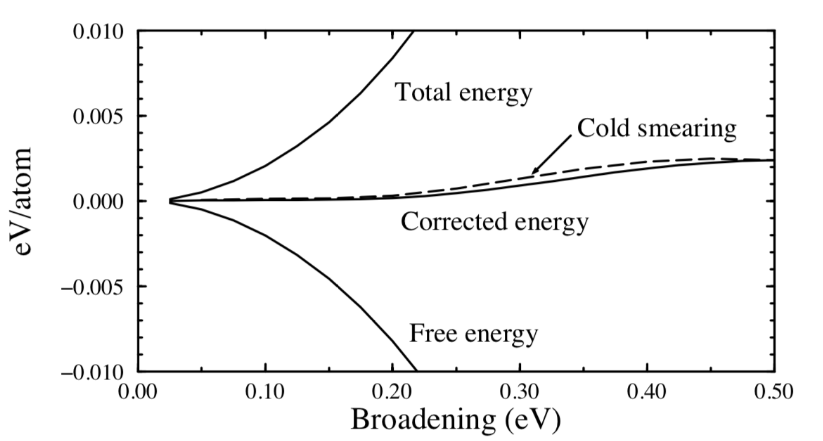
\includegraphics[scale = 0.6]{figs/D2/smearing.png}

  \definicion{I have seen the discussion about relax in zoom. When we should use "relax" instead of "vc-relax"? I have seen  "relax " in papers related to molecules ( with complex carbon structures) is this a correct approach?}

  in general I'd use vc-relax only to obtain the DFT lattice parameters of the crystal bulk structure, which are typically slightly different than the experimental ones. For trying different atomic configurations in the cell relax should be used (after you already obtained appropriate cell parameters) , but it will be discussed tomorrow yes

  \definicion{if we have a ferromagnetic system, how do we know in which direction the magnetization vector is pointing? Where do we find the components of the magnetization vector?}

  In order to know this information, you need to setup a non-collinear calculations with spin-orbit-  in  this way you can explore different directions of the magnetitazion and
  the relative energy differences for each specific direction you fix in
  the input file.
  You can even setup a constrained magnetic moment calculations to adress these energy differences-
  When
  performing non-collinear calculations, in the output file you access to
  the cartesian components of the magnetization for each magnetic atoms-

  \definicion{In the case of a defect calculation, should I first converge the supercell size or is it better to converge first ecut, kpoints, etc., on a smaller cell and do the cell size convergence after?}

  a smaller cell is better, but you have to keep the density of k-points consistent.

  I think its better if you first converge the  ecut and kpoints and than the supercell size.

  \definicion{Thank you! Regarding the reducing number of the k points, if the k-points converged for 8x8x8 in a 2x2x2 supercell and I need a 3x3x3 supercell, which k-points can I use (as it is not a divisor)? Should I round up (6x6x6)?}

  closest integer, preferably rounded up

  \definicion{Question: What is the criteria for cartegorizing a magnetic material as antiferromagnetic or ferromagnetic with respect to the total magnetization, absolute magnetization and magnetic moment?}

  For ferromagnetic materials, the total and absolute magnetization are (almost) the same. For AFM, total magnetization is 0, absolute magnetization is not.

  \definicion{I have a question. If we use very high E\_cut in PAW e.g. 120Ry with E\_rho = 4E\_cut, will the result be acceptable?}

  Likely yes, but it is not a smart (that is: efficient) choice. The higher Ecut means the more cost of CPU.


  \definicion{Another question is, If I do not have metal, is better to use gauss smearing?}

  For insulators you usually don’t need smearing. In case if you use it for getting faster convergence use gaussian smearing with a very small degauss value.

  \definicion{Why did the professor  use starting magnetization 0.6 and -0.6 for AFM iron? My question is about the number, can I use 0.5 and -0.5 or even 1 and -1? Is there  a restricción?}

  you can also start with 0.5. it will converge at the end. If you have rough idea about the number, the simulation will be faster. What you provide is just an initial guess. The code will eventually converge to you different value

  \definicion{I got some doubts about testing convergence. Suppose I've got a slab of an insulator inside a supercell with, let's say, 20 atoms (10 of element A and 10 of element B) and it's the minimal slab I need (I can create greater surfaces multiplaying this "unit" in the xy plane)
  1. How should I run the tests for the cutoffs? I mean should I sweep values for the whole slab or how?
  Suppose now that in order to converge I need to add smearing.
  2. What should be my "first choice" since it's an insulator: gauss or MV?
  3. Since it's not a metal I understand that the smearing contribution should be the least possible. Can I apply the same criterion we used in the hands-on (there was a 3D system and here it is a slab)? There we said that the we considered the convergence achieved with 1mRy/atom so here I should seek for a value of smearing contribution to be lesser than 20mRy?}

  1.) the ecutwfc and ecutrho are properties of the pseudopotential, so you only have to test it for each atomic type in your system (2 in your example), you can do the test for the isolated atom or the bulk structure of the crystal, then you use the highest/hardest cutoff for your supercell calculation. the cell size shouldn't matter for the ecut, what matters is that the energy doesn't change once you increase the cutoff further

  2.) the smearing is a bit more difficult, but you can use mv/mp for insulators as well, but the smearing there should be really small (no bigger than 0.01 Ry), basically you add it only to help in the convergence, once you choose it keep it the same for all calculations (supercells included), so in principle you can determine it for the bulk of the insulator, note that the 0.001 Ry/atom is the criterion for the cutoff not the smearing typically.

  in any case keep an eye on the smearing contribution written in the output and make sure its not significant and at least consistent between different calculations

\section{Hands-on}

    \definicion{Topic:} SCF calculations + post-processing – part 2. Exercises.

    \definicion{Speaker:}	Anton KOKALJ (Jožef Stefan Institute, Slovenia).

\subsection{Si}

\subsubsection{Objetivo}

  Estudiar la convergencia de cálculos pw.x para diferentes Si bulk: primero se estudia la convergencia del cutoff para las funciones de onda ($ecutwfc$) y luego la convergencia para los puntos $k$.

  Las pruebas de convergencia se llevan a cabo haciendo una siere de cálculos variando algún parámetro. Para esto se pueden utilizar shell scripts o PWTK scripts. La diferencia entre estos peuede observarse al comparar, por ejemplo, ex1.ecutwfc.classic/ecutwfc.sh con ex1.ecutwfc/ecutwfc.pwtk, respectivamente.

  La lógica a seguir es la siguiente:
    \begin{enumerate}
      \item Convergencia de la base ($ecutwfc$).
      \item Convergencia de los puntos $k$, utilizando el valor óptimo de $ecutwfc$.
      \item Convergencia del parámetro de red, utilizando los valores óptimos para $ecutwfc$ y la grilla de puntos $k$.
      \item Calcular la estructura de bandas, utilizando los valores óptimos para $ecutwfc$, la $k$-grilla y el parámetro de red.
    \end{enumerate}

\subsubsection{Pasos}

    \begin{enumerate}
      \item Convergencia de $ecutwfc$: correr alguno de los siguientes comandos a gusto.
        \begin{verbatim}
          ./ecutwfc.sh         (shell)
          pwtk ecutwfc.pwtk    (PWTK)
        \end{verbatim}
      \item Convergencia de $k$-grid.
        \begin{verbatim}
          pwtk kpoints.pwtk
        \end{verbatim}
      \item Convergencia del parámetro de red: agregar parámetros necesarios al script antes de correr. Primero corre pw.x y luego ev.x para obtener el parámetro de red y el módulo de Young recurriedno a la ecuación de estado de Murnaghan.
        \begin{verbatim}
          pwtk alat.pwtk
        \end{verbatim}
      \item Estructura de bandas: agregar parámetros necesarios al script antes de correr. Luego de la corrida, poner la energía de Fermi adecuada en el archivo plot.gp. Regraficar la estructura de bandas.
        \begin{verbatim}
          pwtk bands.pwtk
          grep 'highest occupied level' pw.Si.scf.out
          gnuplot plot.gp
        \end{verbatim}
    \end{enumerate}

\subsubsection{Resultados: Si}

  Para los cálculos se utilizaron NCPP con LDA (PZ) como funcional: Si.pz-vbc.UPF.

  Para examinar cómo avanza la autoconsistencia, podemos ejecutar
  \begin{verbatim}
    grep -e "total energy" -e estimated output\_file.out
  \end{verbatim}

  Notar que hay 9 elecctrones dentro de la celda ya que hay 2 átomos por celda con 4 electrones cada uno. Como el sistema es no magnético y es aislante, sólo se computan las 4 ($=\sfrac{8}{2}$) bandas de valencia (estados KS) más bajas.

  Es recomendable usar PWTK ya que está hecho explícitamente para funcionar con QE: la sintáxis se mantiene como en el input original.

  \begin{figure}[H]
      \centering
      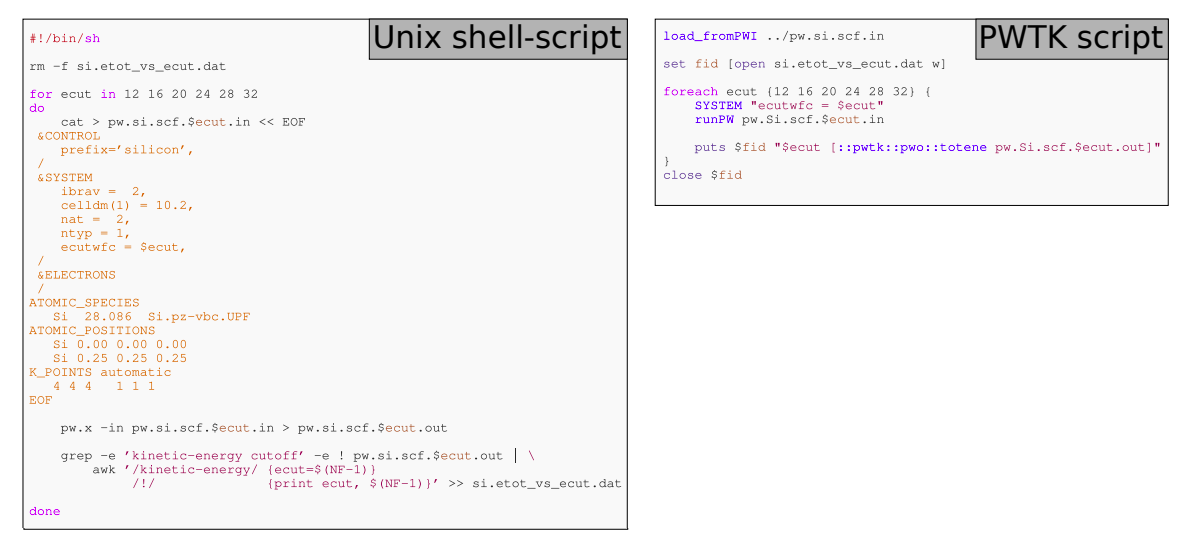
\includegraphics[scale = 0.4]{figs/D2/shellvspwtk.png}
      \caption{Comparación de un script en shell y uno en PWTK.}
  \end{figure}

  Los PWTK scripts son Tcl-scripts donde:
    \begin{itemize}
      \item Se mantienen los nombres de las namelists y las cards, salvo contadas excepciones. Su contenido debe ir entre corchetes (pensarlo como una función de C).
      \item Se pueden escribir tanto números como expresiones matemáticas, pero no debe haber espacios que separen los términos y factores de la expresión.
      \item Se puede indexar usando, por ejemplo, los nombres de los átomos.
      \item Es casesensitive, pero el orden de las namelists y las cards no es importante.
      \item Las variables de los namelists pueden configurarse on-the-fly.
      \item Tanto las namelists como las cards pueden ser llamadas múltiples veces. Sin embargo, PWTK no las considera de igual forma: las cards son tratadas en overwrite mode, mientras que las namelists son tratadas en append mode.
      \item Para desactivar una variable dentro de una namelist basta con darle un valor vacío, \emph{i.e.} no poner nada después del igual.
    \end{itemize}

    Algunas de las funciones que se usan de PWTK en este hands-on son:
      \begin{itemize}
        \item \textbf{load\_fromPWI:} carga input data desde un input de pw.x existente.
        \item \textbf{pwo\_totene:} devuelve la energía total de un output de pw.x.
        \item \textbf{seq:} devuelve una secuencia de números. El primero y el último número son los extremos del intervalo (cerrado). El valor del medio indica el salto.
        \item \textbf{runPW / runPP / runDOS / runPROJWFC:} construye un input file del programa dado (PW, PP, DOS o PROJWFC) y corre el cálculo.
      \end{itemize}

    Respecto al barrido de $ecutwfc$, asumimos que el sistema es convergente cuando la diferencia entre los valores de energía total entre dos mediciones sucesivas de $ecutwfc$ es menor que $1\ \sfrac{mRy}{\sfrac{atom}{cell}}$. En este caso tenemos 2 átomos por celda así que serían $2\ mRy$. De la gráfica podemos pensar que 24 Ry sería suficiente. En números:
      $E_{tot} (24 Ry) = -15.8508\ Ry \wedge E_{tot} (20 Ry) = -15.8475\ Ry \Rightarrow \Delta E_{tot} = 0.0033\ Ry = 3.3\ mRy$

      $E_{tot} (24 Ry) = -15.8508\ Ry \wedge E_{tot} (28 Ry) = -15.8519\ Ry \Rightarrow \Delta E_{tot} = 0.0011\ Ry = 1.1\ mRy$

    Se concluye entones que el valor óptimo es $ecutwfc = 24$.

      \begin{figure}[H]
          \centering
          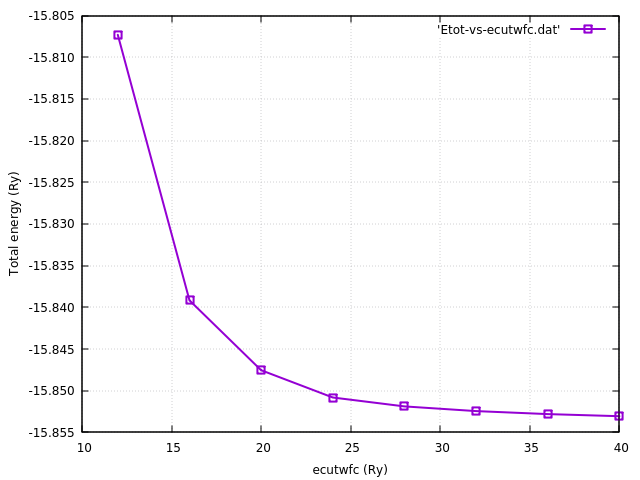
\includegraphics[scale = 0.6]{figs/D2/Si_ecutwfc.png}
          \caption{Barrido de $ecutwfc$ para Si bulk.}
      \end{figure}

    Ahora hacemos el barrido de la $k$-mesh. Consideramos el mismo criterio de convergencia.
      $E_{tot} (222) = -15.7945\ Ry \wedge E_{tot} (444) = -15.8073\ Ry \Rightarrow \Delta E_{tot} = 0.0128\ Ry = 12.8\ mRy$

      $E_{tot} (444) = -15.8073\ Ry \wedge E_{tot} (666) = -15.8076\ Ry \Rightarrow \Delta E_{tot} = 0.0003\ Ry = 0.3\ mRy$

    Se concluye entones que el valor óptimo es $4\ 4\ 4$.

      \begin{figure}[H]
          \centering
          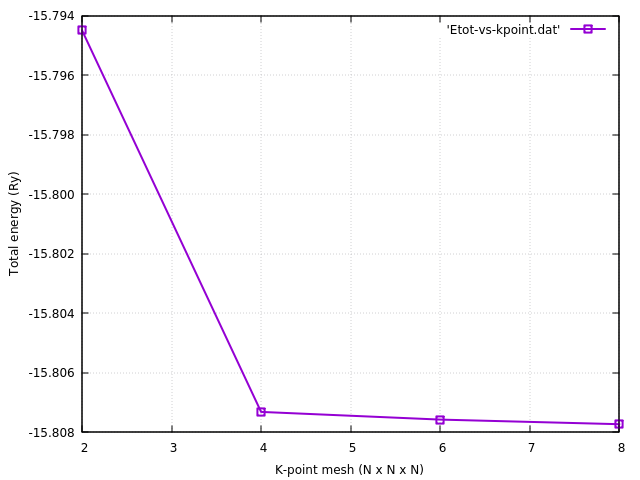
\includegraphics[scale = 0.6]{figs/D2/Si_k.png}
          \caption{Barrido de $k$-mesh para Si bulk.}
      \end{figure}

    \Obs{La convergencia de los puntos k no es necesariamente monotónica ya que no existe ningun principio variacional con respecto al número de puntos k.}

    Ahora analizamos el parámetro de red. El equilibrio en el caso del Si queda determinado por aquel parámetro de red que minimiza la energía ya que no hay fuerzas actuando sobre los átomos dada la simetría.

    \Obs{La ausencia de fuerzas debida a la simetría puede chequearse haciedno $tprnfor=.tru.$ en \&CONTROl.}

    De la gráfica vemos que es $10.2\ Bohr$. Siendo más precisos, la ecuación de estado nos dice que es $10.2090\ Bohr$ y el módulo de Young es $934\ kbar$.

    A partir de los resultados de la ecuación de estado, notamos además que para parámetros de red menores al óptimo, la energía total es menor que la entalpía. Lo opuesto ocurre para parámetros de red mayores al óptimo.

      \begin{figure}[H]
          \centering
          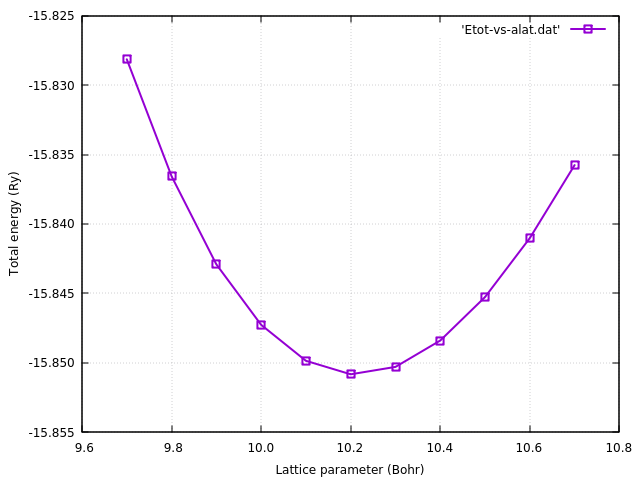
\includegraphics[scale = 0.6]{figs/D2/Si_alat.png}
          \caption{Barrido del parámetro de red para Si bulk.}
      \end{figure}

      \begin{figure}[H]
          \centering
          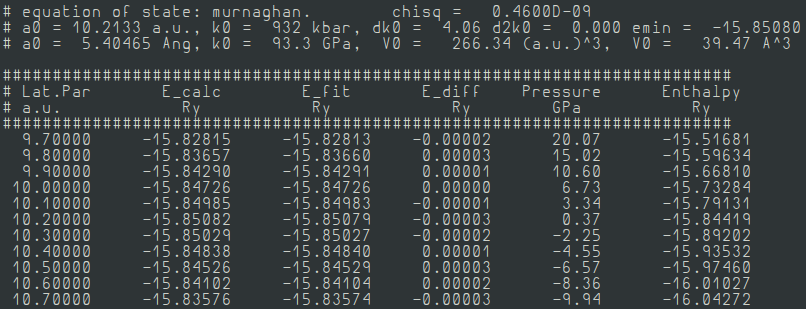
\includegraphics[scale = 0.6]{figs/D2/Si_mur.png}
          \caption{Resultados del fiteo utilizando la ecuación de estado.}
      \end{figure}

    Para hacer el cálculo de bandas, no podemos usar el mesh corrido, sino los valores serán erróneos: no estaríamos incluyendo el punto $\Gamma$.

    \begin{figure}[H]
        \centering
        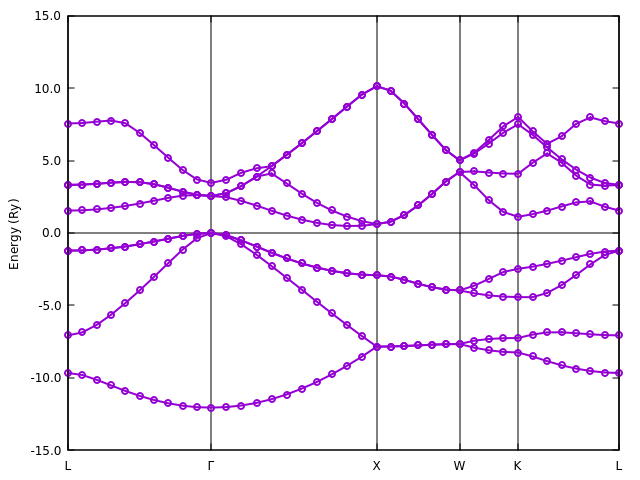
\includegraphics[scale = 0.6]{figs/D2/Si_bands.png}
        \caption{Estructura de bandas para Si bulk.}
    \end{figure}

  Al analizar las curvas de energía total en función del parámetro de red para diferentes $k$-mesh y $ecutwfc$ vemos que:
    \begin{itemize}
      \item Para un mismo $ecutwfc$, la energía no es tan sensible al $k$-mesh: con 2x2x2 es muy mala la convergencia, pero ya con 4x4x4 se estabiliza.
      \item A medida que aumentamos $ecutwfc$, las curvas se van desplazando hacia valores más negativos de energía.
    \end{itemize}

  Al comparar los $k$-mesh volvemos a elegir 4x4x4. Al comparar los mínimos, vemos que la elección de 24 Ry fue acertada.

  \begin{figure}[H]
      \centering
      \subfigure[]{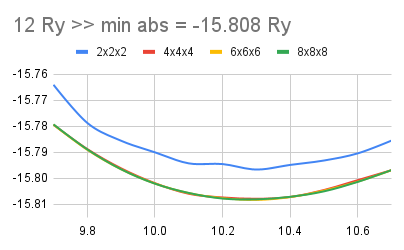
\includegraphics[scale = 0.55]{figs/D2/alat/12.png}}
      \subfigure[]{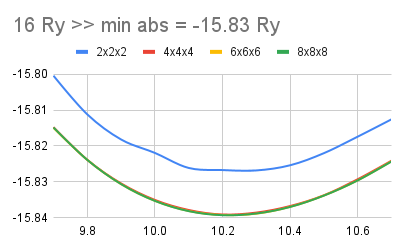
\includegraphics[scale = 0.55]{figs/D2/alat/16.png}} \\
      \subfigure[]{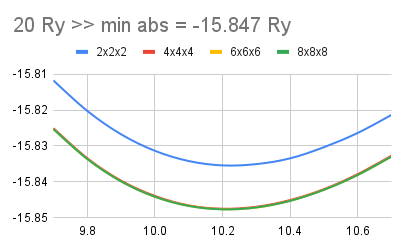
\includegraphics[scale = 0.55]{figs/D2/alat/20.png}}
      \subfigure[]{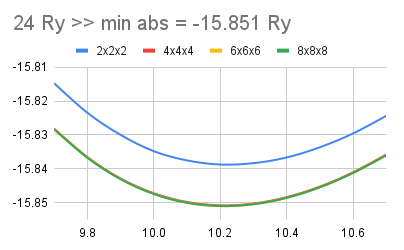
\includegraphics[scale = 0.55]{figs/D2/alat/24.png}} \\
      \subfigure[]{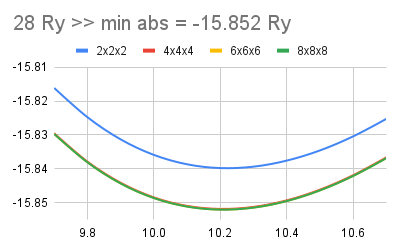
\includegraphics[scale = 0.55]{figs/D2/alat/28.png}}
      \subfigure[]{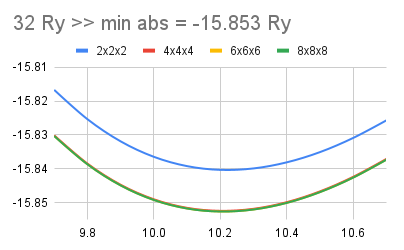
\includegraphics[scale = 0.55]{figs/D2/alat/32.png}} \\
      \subfigure[]{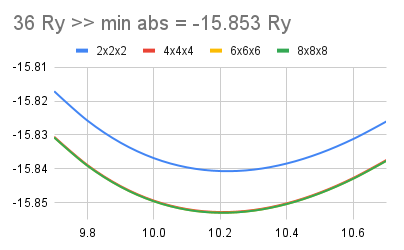
\includegraphics[scale = 0.55]{figs/D2/alat/36.png}}
      \subfigure[]{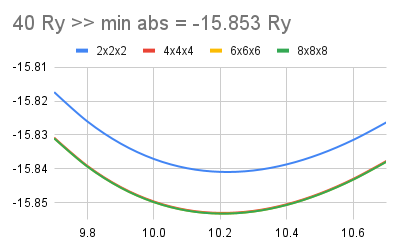
\includegraphics[scale = 0.55]{figs/D2/alat/40.png}} \\
      \caption{Energía en total en función del parámetro de red para diferentes cutoff y diferentes $k$-mesh.}
  \end{figure}


\subsection{Al}

\subsubsection{Objetivo}

  Cálculo de sistemas metálicos: Al bulk.

  Se explora diferentes esquemas de smearing: cómo hacerlo y hasta dónde. Se plotea la densidad de carga electrónica.

\subsubsection{Pasos}

    \begin{enumerate}
      \item Explorar qué hace el smearing con función de ensanchamiento Gaussiana. Una vez que corra, edirar el .pwtk y agregar más puntos de degauss, como 0.15 ó 0.2, dentro del foreach. Para evitar volver a correr lo ya corrido, encender el modo $restart$ (descome $\#restart\ true$).
        \begin{verbatim}
          pwtk degauss.pwtk
        \end{verbatim}
      \item Calcular la densidad de carga (chdens).
        \begin{enumerate}
          \item \textbf{1-chdens.pwtk:}
            Calcular la densidad de carga de valencia. Editar con las variables adecuadas antes de correr. Ver la densidad de carga con xcrysden.
            \begin{verbatim}
              pwtk 1-chdens.pwtk
            \end{verbatim}
          \item \textbf{2-chdens-paw.pwtk:}
            Calcular la densidad de carga all-electron tanto de valencia como total, mediante el uso de PAWPP. Ver en xcrysden.
            \begin{verbatim}
              pwtk 2-chdens-paw.pwtk
              xcrysden --xsf all-electron-VALENCE-chdens.xsf -s state2.xcrysden
              xcrysden --xsf all-electron-total-chdens.xsf  -s state2.xcrysden
            \end{verbatim}
        \end{enumerate}
    \end{enumerate}

\subsubsection{Resultados: Al}

Aunque Al es más simple que Si ya que tiene sólo un átomo por celda dentro de una FCC, se trata de un metal: no será suficiente con sólo conocer las bandas de valecias y pocos puntos k.

El barrido de parámetros es tridimensional: se analizan los puntos k, el tipo de smearing y el valor propio del smearing que se utiliza.

Cuando usamos $g$ (gaussian) vemos que la mesh 4x4x4 no es útil para Al como lo era para Si. A mayor smearing, las curvas convergen unas a otras. Con esto en mente, podríamos usar smearing más altos y una mesh con menos resolución. Cuando usamos $m-p$ o $m-v$ queda claro que la energía no depende tan fuertemente del smearing como en el caso anterior, permitiendo una convergencia más rápida y segura. En el caso del aluminio tenemos entonces que una buena convergencia podría alcanzarse usando $m-p$ o $m-v$ con un mesh 12x12x12 y un $degauss$ entre 0.01 y 0.05 Ry.

El ensanchamiento no puede reducirse demasiado: los niveles energéticos deben tener cierta superposición (es un metal) o de lo contrario la ventaja de hacer smearing se terminaría perdiendo. En otras palabras: valores de degauss muy altos empiezan a romper todo.

  \begin{figure}[H]
      \centering
      \subfigure[]{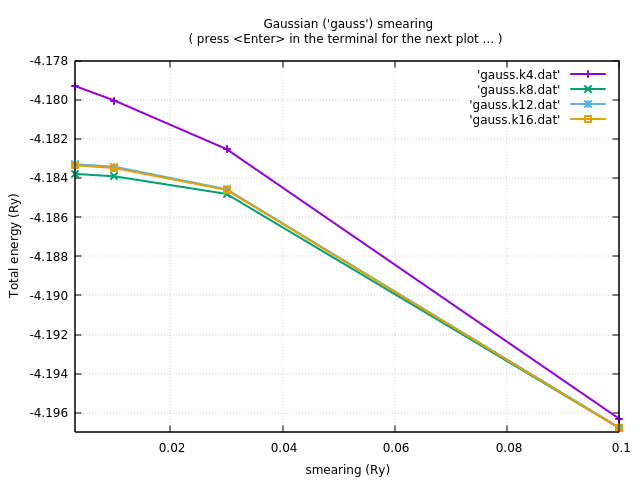
\includegraphics[scale = 0.45]{figs/D2/Al_gauss.png}}
      \subfigure[]{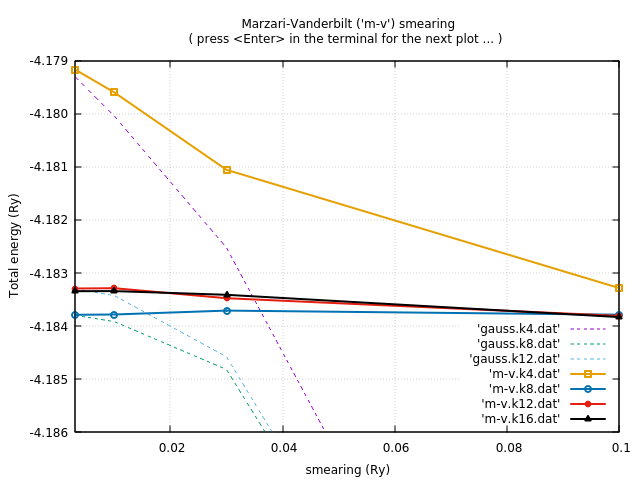
\includegraphics[scale = 0.45]{figs/D2/Al_mv.png}}
      \subfigure[]{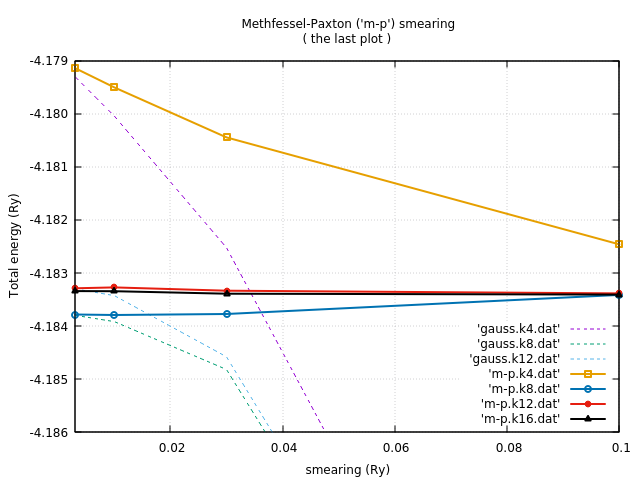
\includegraphics[scale = 0.45]{figs/D2/Al_mp.png}}
      \caption{Energía total en función del smearing y el ancho de smearing utilizado, variando la cantidad de puntos K. Las ocupaciones son: g (a), m-v (b) y m-p (c).}
  \end{figure}

  Dejando de lado los test de convergencia, vamos a ver cómo hacer un post-processing, determinando la densdiad de carga. La calculamos con dos potenciales diferentes:
    \begin{itemize}
      \item Un PP: Al.pz-vbc.UPF
      \item Un PAWPP para hacer un all-electron: Al.pbe-n-kjpaw\_psl.1.0.0.UPF
    \end{itemize}

  Las corridas con all-electron requieren cutoff gigantes (ecutrho ~ 1000 Ry). A partir de las figuras vemos que usando PP no hay electrones en torno a los núcleos, sino sólo en zonas intersticiales. Esto es por la manera en la que justamente construimos los PP. Para el caso del all-electron, se grafica valencia y full según el input del pp.x que le demos ($plot\_num$). En este caso sí se aprecia carga en torno al núcleo: es totalmente brillante debido a la alta concentración y localización de los electrones del core.

  \begin{figure}[H]
      \centering
      \subfigure[]{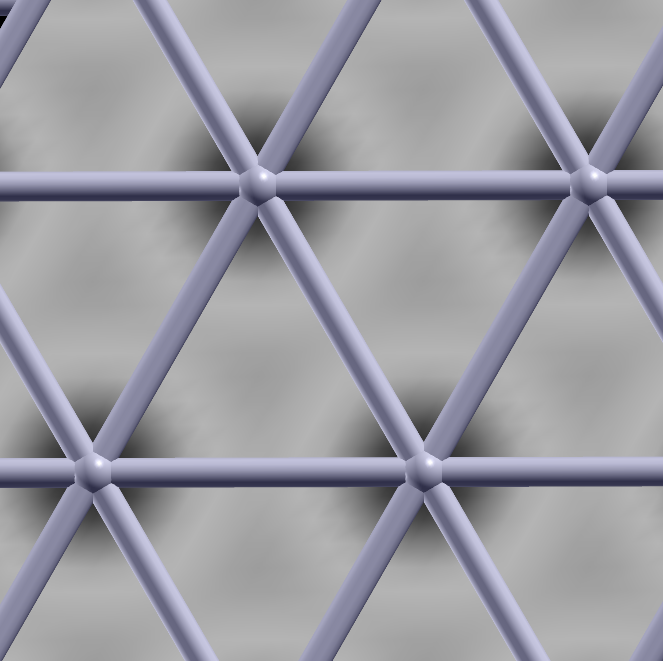
\includegraphics[scale = 0.35]{figs/D2/Al_chdens1.png}}
      \subfigure[]{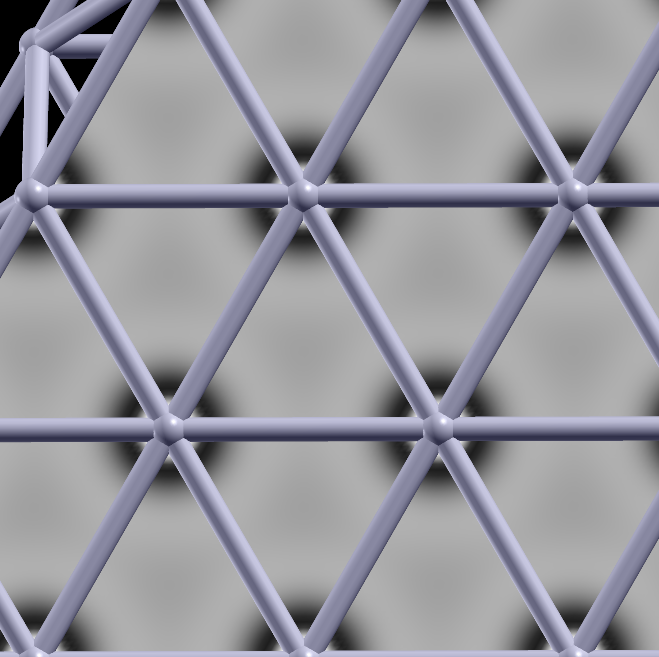
\includegraphics[scale = 0.35]{figs/D2/Al_chdens2_val.png}}
      \subfigure[]{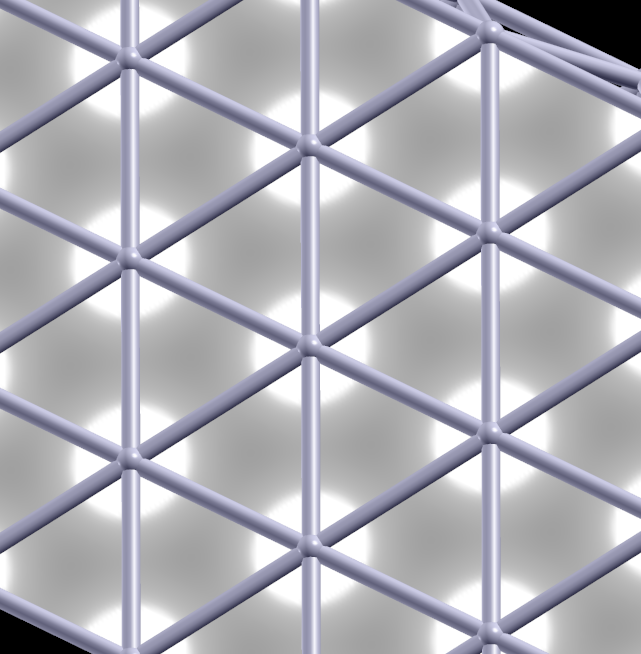
\includegraphics[scale = 0.35]{figs/D2/Al_chdens2_total.png}}
      \caption{Densidad de carga obtenida a partir de dos potenciales diferentes. Negro implica que no hay cargas y cuanto más brillante, mas carga hay. En (a) se usa el PP mientras que en los otros se usan el all-electron: (b) sólo valencia y (c) todo.}
  \end{figure}

\subsection{Fe}

\subsubsection{Objetivo}

  Realizar cálculos con sistemas magnéticos (bulk de Fe tanto ferromagnetico como antiferromagnetico). Aprender criterios de convergencias para USPP: el parámetro dual. Plotear DOS total y proyectada (PDOS) sobre los orbitales s y d.

\subsubsection{Pasos}

  Las diferencias entre los códigos ferromagnetico y antiferromagnetico pueden verse con
  \begin{verbatim}
    diff pw.fe\_fm.scf.in pw.fe\_afm.scf.in
  \end{verbatim}

  Los cálculos se pueden correr con
  \begin{verbatim}
    pw.x < pw.fe\_fm.scf.in > pw.fe\_fm.scf.out
    pw.x < pw.fe\_afm.scf.in > pw.fe\_afm.scf.out
  \end{verbatim}

  Analizar los outputs, prestando atención a los valores total/absolute magnetization en ambos casos.

    \begin{enumerate}
      \item Realizar un test de convergencia específico para USPP.
        \begin{verbatim}
          pwtk ecut.pwtk
        \end{verbatim}
      \item Calcular y plotear DOS y PDOS sobre OA s y d. Antes de correr, ingresar los valore adecuados de las variables necesarias. Luego poner el valor correcto de la energía de Fermi en plot.gp para después hacer el plot.
        \begin{verbatim}
          pwtk dos.pwtk
          grep 'Fermi energy' pw.Fe.nscf.out
          gnuplot plot.gp
        \end{verbatim}
    \end{enumerate}

\subsubsection{Resultados: Fe}

  En la siguiente figura se aprecia la diferencia entre ambos archivos, siendo primero el ferromagnetico y el segundo el antiferromagnetico.

    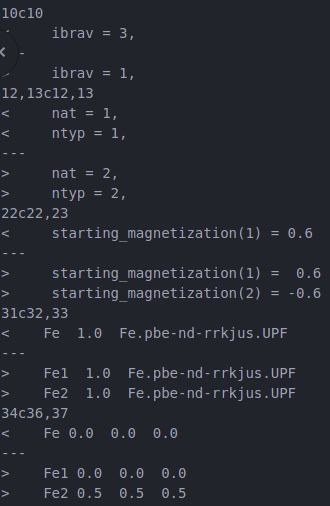
\includegraphics[scale = 0.45]{figs/D2/Fe_diff.png}

  Como vamos a usar un USPP (Fe.pbe-nd-rrkjus.UPF) debemos analizar la convergencia del $ecutrho$ también: tener $dual=4$ no será suficiente.
    $$dual = \frac{ecutrho}{ecutwfc}$$

  \Obs{Se puede estudiar también la variación del resultado respecto a la CI de la magnetización.}

  Al correr ambos  programas vemos que para el caso ferromagnetico la magnetización total es de 2.29 Bohr mag/cell y la absoluta es de 2.45 Bohr mag/cell, mientras que para el caso antiferromagnetico la total es 0 y la absoluta es 4.13 Bohr mag/cell.

  Ahora vamos a analizar la convergencia de los cutoffs con el caso ferromagnetico. Para ello se hace un barrido de dual y, para cada uno de ellos, se prueban diferentes ecutwfc. Vemos que para un dual de 4 tenemos una curva, pero para los duales 8 y 12 las curvas coinciden. Si queremos usar el dual de 4 debemos usar $ecutwfc > 40$; en cambio con los otros duales podemos usar $ecutwfc = 25$. En el código se hacen muchísimas más operaciones con las funciones de onda que con las densidades de carga, por lo que si usamos un $ecutwfc$ más chico el cálculo irá nás rápido.
    \begin{figure}[H]
        \centering
        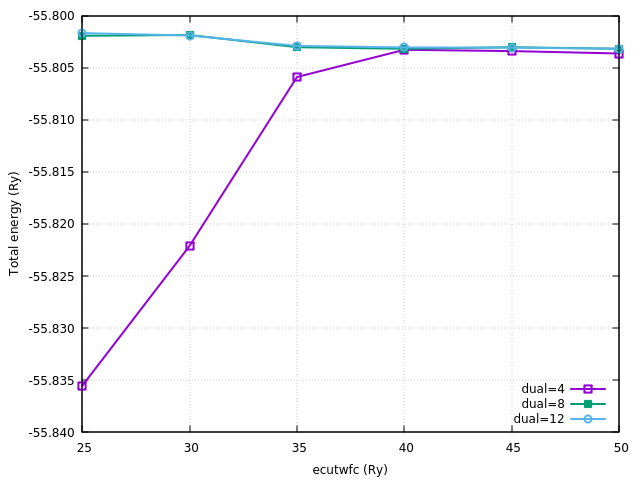
\includegraphics[scale = 0.45]{figs/D2/Fe_fm_dual.png}
        \caption{Variación de la energía total en función del dual para Fe ferromagnetico.}
    \end{figure}

  Ahora vamos a graficar DOS y PDOS, también para el caso ferromagnetico. Recordamos que necesitamos una $k$-mesh más densa. Además $occupations = 'tetrahedra'$ suele ser útil para este tipo de cálculos. En la DOS vemos que hay más estados ocupados con spin up que down. En la PDOS vemos que
    \begin{itemize}
      \item Las bandas s son muy anchas y bajas: los 2 electrones por átomo en el orbital s ocupan un rango muy grande de energía (~ 15 eV).
      \item Las bandas d son más picudas: tenemos 10 electrones por átomo en un rango energético de ~ 5 eV.
    \end{itemize}

  En realidad falta considerar la energía de Fermi. A partir de la misma, vemos que sólo hay 1 electrón en el s y 7 en el d. Esto también explica el gran pico de spin down a valores tan grandes de energía: estamos muy por encima de la energía de Fermi (antiorbitales).

  \begin{figure}[H]
      \centering
      \subfigure[]{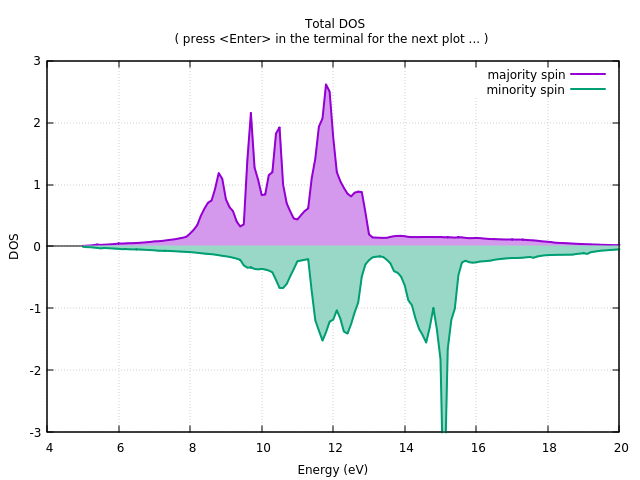
\includegraphics[scale = 0.5]{figs/D2/Fe_DOS.png}}
      \subfigure[]{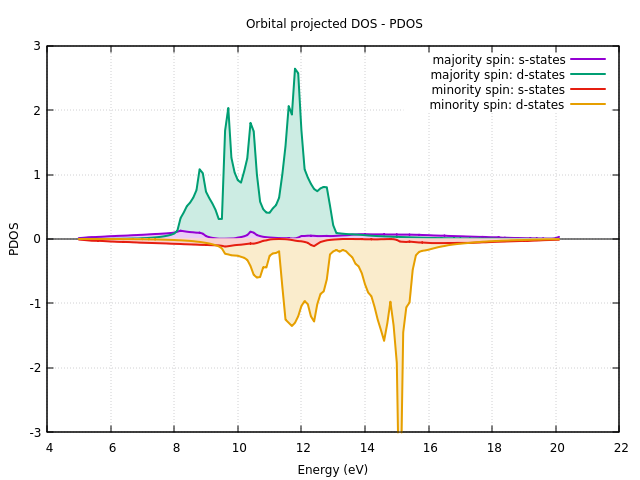
\includegraphics[scale = 0.5]{figs/D2/Fe_PDOS.png}}
      \caption{DOS y PDOS sobre los OA s y d para el Fe ferromagnetico. Majority y minority spin corresponden a spin up y down, respectivamente.}
  \end{figure}


    \chapter{Día 3}

      \section{Teórico 1/2}

  \definicion{Topic:} Forces, stresses, geometry optimisation.

  \definicion{Speaker:}	Pietro DELUGAS (SISSA, Italy).

\subsection{Parámetros estructurales}

  Un sistema queda definido a partir del número y tipo de iones, donde el tipo queda descripto a partir del PP, junto a las posiciones que ocupa cada uno, determinando la estructura.

  La estructura de un sistema periódico queda descripta por:
    \begin{itemize}
      \item Los parámetros de red: $\vec{a}_1$, $\vec{a}_2$ y $\vec{a}_3$.
      \item Las posiciones atómicas: $\vec{r}_I$
    \end{itemize}

  Como la modificación de los parámetros de red alteran las posiciones atómicas, se utilizan coordenadas cristalinas fraccionarias, donde la posición atómica queda expresada a partir de los parámetros de red.
    $$\vec{r}_I = \sum_{i=1}^3 x_i \vec{a}_i \quad ; \quad 0 \leq x_i \leq 1$$

  La energía potencial $E(\vec{r}_I, \vec{a}_i)$ termina siendo la PES (Potential Energy Surface) del sistema bajo la aproximación de Born-Oppenheimer: esta es la función a minimizar.

\subsection{Fuerzas}

  La PES debe ser derivable ya que la fuerza es el opuesto de la derivada de las interacciones interelectrónicas e internucleares respecto a las posiciones.
    $$F_I = - F_I^{el} - \frac{e^2}{2} \frac{\partial}{\partial \vec{r}_I} \sum_{I\neq J} \frac{Z_I Z_J}{\norm{\vec{r_I} - \vec{r_J}}}$$

  El teorema de Hellmann-Feynman puede ser aplicado en DFT. El mismo establece que la derivada de la energía total $E$ respecto a un parámetro continuo $\lambda$ es igual al valor de expectación de la derivada del Hamiltoniano respecto a dicho parámtro. Así, una vez que la distribución espacial de los electrones ha sido determinada al resolver la ecuación de Schrödinger, todas las fuerzas del sistema puede usarse recurriendo a la electrostática clásica.
    $$\frac{d E}{d \lambda} = \expval{\sfrac{d H}{d \lambda}}{\Psi}$$

  De este modo, la contribución electrónica $F_I^{el}$ puede determinarse como el valor de expectación de las derivadas del potencial externo aplicado.
    $$F_I^{el} = - \frac{\partial E}{\partial \vec{r}_I} = - \sum_v f_v \expval{\sfrac{\partial V}{\partial \vec{r}_I}}{\psi_v} = - \int n(\vec{r}) \frac{\partial V}{\partial \vec{r}_I} d \vec{r}$$

  La idea de calcular las fuerzas como un valor de expectación es válida sólo si estamos realmente en convergencia: la precisión de las fuerzas dependerá de que estemos cerca de la autoconsistencia. Esto se debe a que en realidad tenemos un segundo término al derivar la energía, el cual se anula cuando estamos en un mínimo:
    $$\frac{\partial E}{\partial \vec{r}_I} = \int n(\vec{r}) \frac{\partial V}{\partial \vec{r}_I} d \vec{r} + \int \frac{\delta E}{\delta n(\vec{r})} \frac{\partial n (\vec{r})}{\partial \vec{r}_I} d \vec{r}$$

  En QE, pw.x imprime un estimado de este segundo término al final de la autoconsistencia que puede servir como una correción aproximada. Durante una relajación o una dinámica debemos monitorear estos valores: deben ser algún orden de magnitud menor que las fuerzas calculadas. De lo contrario el programa emite una advertencia.

\subsection{Tensión y estrés}

  Dijimos que cambiar los valores de los parámetros de red implica una deformación uniforme del sistema. Esta queda descripta por el tensor de tensión $e_{\alpha \beta}$. La transformación es lineal
    $$\vec{r}_{\alpha}^{'} = \sum_{\beta} (\delta_{\alpha \beta} + e_{\alpha \beta}) \vec{r}_{\beta}$$

  El tensor de estrés es la derivada de la energía por unidad de volumen con respecto a la tensión.
    $$\sigma_{\alpha \beta} = -\frac{1}{\Omega} \frac{\partial E}{\partial e_{\alpha \beta}}$$

  Sólo la contribución simétrica del tensor $e_{\alpha \beta}$ da lugar a una deformación efectiva, afectando la energía, ya que la contribución antisimétrica es simplemente una rotación.

  La traza del tensor de estrés está relacionada a la presión según
    $$P = \frac{1}{3} \sum_{\alpha} \sigma_{\alpha \alpha} $$

  mientras que las componentes no diagonales son el estrés de corte (deformaciones no paraleas a los planos de la celda unidad).

  Como el estrés es una primera derivada de un parámetro externo, el teorema de Hellmann-Feynman puede aplicarse. En este caso no depende explícitamente de las posiciones iónicas, sino que es la derivada de la energía cinética, la de Hartree y la de XC con respecto a una deformación uniforme. Esto lleva a que involucra las componentes de las funciones de onda, las cuales dependen a su vez de la base de PWs usada.

\subsubsection{Smooth cutoff}

  Evaluar la energía y el estrés puede dar discontinuidades si el cutoff no fue convergente, teniendo que usar valores más grandes. Una alternativa es usar smooth cutoff: creamos una región donde las PW entran y salen del conjunto base con regularidad, teniéndose en cuenta cuando se evalúa el estrés y la energía.

  Esto se logra modificando el funcional de energía cinética por lo que las PW de borde se vuelven caras.
    $$T (\vec{G}) = \underbrace{\norm{\vec{G}}^2}_{\text{original}} + \underbrace{Q_{cut} \left[ 1 + erf\left( \frac{\norm{\vec{G}}^2 - E_{cfix}}{\sigma} \right) \right]}_{\text{smooth}}$$

  Cuando $\vec{G}^2 - E_{cfix} < 0 \wedge \abs{\vec{G}^2 - E_{cfix}} \ll \sigma $ la función error tiende a $-1$, por lo que $T (\vec{G}) \rightarrow \norm{\vec{G}}^2$. A medida que $\vec{G}^2$, empieza a haber contribuciones no nulas. Sin embargo, la transición es suave y no brusca.

  En QE tengo las siguientes variables del input en pw.x (Fig. \ref{fig:smooth}):
    \begin{itemize}
      \item $ecfied \rightarrow$ energía por encima de la cual las PWs alcanzan el máximo costo.
      \item $qesigma \rightarrow$ ancho a partir del cual se empieza a sumar este costo extra.
      \item $qcutz \rightarrow$ valor del costo extra de energía.
    \end{itemize}

    \begin{figure}[H]
        \centering
        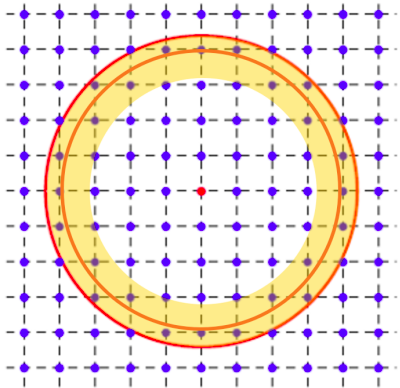
\includegraphics[scale = 0.6]{figs/D3/smooth.png}
        \caption{Cómo afectan las variables del smooth cutoff en la grilla sobre el $G$-espacio: $ecfied$ es el círculo naranja, $qesigma$ es el anillo amarillo t $ecutwfc$ es el círculo rojo.}
        \label{fig:smooth}
    \end{figure}

  Tenemos entonces que el smooth cutoff nos permite hacer una evaluación más regular del estrés y, además, no necesitamos aumentar $ecutwfc$.

\subsection{Métodos de optimización estructural}

  En pw.x se pueden hacer dos tipos de optimizaciones estructurales:
  \begin{enumerate}
    \item Manteniendo fijo el tamaño de celda: $calculation = 'relax'$. Se dan las posiciones atómicas y las mismas cambian según las fuerzas.
    \item Con tamaño de celda variable: $calculation = 'vc-relax'$. Se dan las posiciones atómicas y el tensor de tesión de la celda y las mismas cambian según las fuerzas y el tensor de estrés.
  \end{enumerate}

  Se tienen 2 algoritmos para para relajar:
    \begin{enumerate}
      \item \textbf{BFGS:} es un algoritmo cuasi-Newtoniano. Es el que se hace por defecto: $ion_dynamic='bfgs'$ y $cell_dynamics='bfgs'$
      \item \textbf{Quickmin:} es una dinámica de Verlet amortigüada. Debo decirle $ion_dynamic='damp'$ y $cell_dynamics='damp-pr'$ o $cell_dynamics='damp-w'$
    \end{enumerate}

\subsubsection{Quickmin}

  El mecanismo de amortiguación extrae energía cinética del sistema a medida que el sistema va cayendo al mínimo. Este algoritmo elimina cualquier componente de velocidad generalizada cuya dirección se oponga a la componente conjugada de la fuerza generalizada.

  Aunque el algoritmo es robusto ya que funciona incluso estando lejos del mínimo, requiere cierta experiencia con MD para establecer el time step. Suele ser más lento que BFGS: se suele usar primero un BFGS y luego el quickmin.

\subsubsection{BFGS}

  Es un algoritmo muy útil tanto para celda fija como para celda variable. En las proximidades de un punto de equilibrio $\vec{r}^{eq}$ ($\nabla E (\vec{r}^{eq}) \approx 0$) se asume una forma cuadrática para $E(\vec{r})$ tomando la Hessiana $\mathcal{H}$.
    $$E(\vec{r}) \approx E(\vec{r}^{eq}) + \frac{\vec{r} - \vec{r}^{eq}}{2} \mathcal{H} (\vec{r} - \vec{r}^{eq})$$

  Dados dos puntos $\vec{r}_1$ y $\vec{r}_2$ y sus respectivos gradientes $\vec{g}_1$ y $\vec{g}_2$, se tiene queda $\vec{g}_2 - \vec{g}_1 = \mathcal{H} (\vec{r}_2 - \vec{r}_1)$. Luego $\vec{g}_2=0$ si $\vec{r}_2 = \vec{r}_1 - \mathcal{H}^{-1} \vec{g}_1$ (Paso de Newton-Taphson).

  En la práctica se tiene una secuencai de cálculos en las posiciones $\vec{r}_i$.
    $$\vec{r}_{i+1} = \vec{r}_i + T_k^L \frac{\vec{s}_k^{NR}}{\norm{\vec{s}_k^{NR}}} \quad ; \quad \vec{s}_k^{NR} = - \mathcal{H}_k^{-1} \vec{g}_k$$

  donde $T_k^L$ se conoce como radio de confianza el cual determina cuánto nos vemos en la dirección dictada por $\vec{s}_k^{NR}$.

  Para el paso siguiente debemos actualizar la Hessiana de una manera particular la cual involucra diferencias entre gradientes.

  En cada uno de los pasos también se actualiza $T_k^L$ de manera tal que satisfaga las dos condiciones de Wolfe:
    \begin{enumerate}
      \item \textbf{Decrecimiento suficiente:} la nueva energía debe ser menor que cierto valor, sino $T_k^L$ debe acortarse.
        $$E_{new} \leq E_{old} + \omega_1 T_k^L \vec{g}\cdot \vec{s}_k$$
      \item \textbf{Curvatura:} si la nueva pendiente es muy alta, el $T_k^L$ es aumentado.
        $$\vec{g}_{new} \cdot \vec{s}_k \geq \omega_2 \vec{g}_{old} \cdot \vec{s}_k$$
    \end{enumerate}

  Los valores $\omega_{1}$ y $\omega_{2}$ se pueden fijar en el input. De lo contrario, el programa usa los valores por default.

\subsubsection{Características de la optimización estructural}

  \begin{itemize}
    \item Permite encontrar únicamente el mínimo más cercano, ya que no tiene la posibilidad de sortear barreras de activación.
    \item En principio no rompe la simetría del cristal, salvo errores por ruido numérico. Esto permite encontrar mínimos atados a la simetría dada puesto que puede haber diferentes mínimos asociadas a distintas simetrías.
    \item Durante una vc-relax el conjunto de PWs se mantiene constante a pesar de que los parámetros de red van cambiando. Esto hace que el resultado final no sea exactamente igual a lo que uno obtendría al comenzar la corrida de cero con el mismo cutoff ya que ambas bases no son iguales. Una vez obtenidos los vectores de red optimizados, el programa recalcula la energía con la base asociada a estos nuevos valores.
    \item Utiliza tanto las energías como las fuerzas para ubicar el mínimo. Si la SCF no fue convergente, el algoritmo no será convergente o dará lugar a errores. El error en las fuerzas es lineal, mientras que el error en las energías es cuadrático.
  \end{itemize}

\subsection{Born-Oppenheimer MD}

  Asumiendo un comportamiento clásico para los núcleos y los electrones en el estado fundamental, recurrimos a un Lagrangiano para describir el movimiento nuclear. Las ecuaciones de movimiento son entonces las ecuaciones de Newton usuales, las cuales pueden discretizarse e integrarse. Esto es lo que se conoce como MD \emph{sobre la superficie BO} donde los electrones se encuentran siempre en su estado fundamental instantáneo.

  El cálculo puede hacerse recurriendo a diversos algoritmos como Verlet o velocity Verlet.

  Algunas cosas a tener en cuenta son:
    \begin{itemize}
      \item El time step debe ser tan grande como sea posible, pero lo suficientemente pequeño como para poder seguir el movimiento nuclear con precisión. Se tiene que
        $$\Delta t \approx 0.01 - 0.1 \Delta t_{max} \quad ; \quad \Delta t_{max} = \frac{1}{\omega_{max}}$$
      donde $\omega_{max}$ es la frecuencia del modo vibracional (fonón) más rápido que tengamos en el sistema.
      \item Las fuerzas deben ser los suficientemente precisas como para que la energía se conserve paso a paso. De lo contrario, se observa un drift energético.
      \item Una BOMD es computacionalmente cara (No me la counter strike). A veces conviene hacer CPMD.
    \end{itemize}

\section{Q\&A 1/2}

    \definicion{Why keep the previous grid during the optimization cycle? Since the meat of the process is: scf --> optimize --> scf --> ... --> convergence ; why does one not consider the new lattice vectors? Why not adjust the cutoff accordingly at every step as it is done in the very last step of the optimization (I think), why keep the ellipse instead of the circle for the entire optimization? Is it a convergence issue?}

    or computational efficiency. reallocating everything is expensive

    \definicion{Does the penalty for high G components you were mentioning (the one with the erf) alleviate these effects or is it unrelated? I have not understood where this applies. I have not used the related flags so far in my calculations, in what cases should I bother with these parameters?}

    yes in principle any G  in the buffer zone has negligible weight in the computation but any G in there enters smoothly in the computation if its lenght become shorter and the stress derivative of the kinetic energy functional takes into account the change in energy of the Gs in the buffer zone

    \definicion{If local minima are an issue can you give a bigger kick to the system in order for it not to get trapped there (something analogous to what happens in ML algorithm since you are in a very similar optimization problem optimized by gradient descent)? Does it make sense to start a calculation with a big kick, see where the problem starts oscillating and then reduce the kick around that point with another calculation (or even do this automatically) ?}

    yes with complicated landscapes there are many methods not implemented directly in QE but that use QE as a force engine

    \definicion{When I do the relax calculation, in the .out file there is the information about the forces. What kind of information does this total force and  DFT-D3 dispersion force give us?}

    the one is just the amount of Forces due to DFT-D3 that is a post-DFT correction to forces. If you see there is also the warning about the fact that the dft forces have a magnitude comparable with the force. They are both very small though you should be close to the minimum

    \definicion{In the relax calculation, what does the 'upscale' parameter do to the ions?}

    Nothing: it sets a maximum value for scf threshold tightening, avoiding to end up with too small scf thresholds and never get to convergence

    \definicion{In which cases I would choose Ion-dynamics instead bfgs?}

    In cases where bfgs doesn't converge it could be useful

    \definicion{there is any way to get a good trade-off between the energy convergence thresh. and the force conv thresh? A general rule}

    Usually its a good idea to stick to the defaults, if you need to relax the system more you can tighten the criteria in a follow up calculation

    \definicion{s there a way to estimate how much memory I will use for the process? My question is because I usually use a cluster and I need to give these information before run a code.}

    There is a memory estimate written in the output of QE

    \definicion{Thinking in the Gamma point trick here, to reduce the expensive cost of optimization, should we use the converged k points or could we assume in general using less points its not going to affect strongly the optimized coordinates. (then use more kpoints in next calculations)}

    Ideally, we use the converged k points. But, as we use a supercell we reduce the k-point accordingly.

    \definicion{why at this example in vc-relaxation, you use 6 6 4 k points, not symmetric?}

    As we use a hexagonal cell, a=b !=c, so having the same k points grid wont be accurate. The value of the k points should be inverse  proportional to the real space distance

    \definicion{Why does it use 'm-p' for Zn? If I do not know, would I do the study of convergence?}

    M-P is one of the best smearing schemes for metallic systems. It could gives very serious problems for insulators.

    \definicion{What is the definition of force convergence threshold? Does it mean that the force of each atom less than the threshold?}

    Yes. Default is 1e-3 Ry/Bohr.

\section{Teórico 2/2}

    \definicion{Topic:} Chasing saddle points: the NEB method.

    \definicion{Speaker:}	Anton KOKALJ (Jožef Stefan Institute, Slovenia).

\subsection{Procesos activados}

  Se conoce como proceso activado a cualquier proceso caracterizado por barreras de activación, las cuales quedan determinadas por los saddle. Dada una PES se tienen infinitos caminos de reacción que conectan el estado inicial con el final. Se conoce como MEP (Minimum Energy Path) al camino de reacción más probable a $0\ K$. Cuando recorremos el MEP, el saddle determina el estado de transición (Fig. \ref{fig:saddle}).

  \begin{figure}[H]
      \centering
      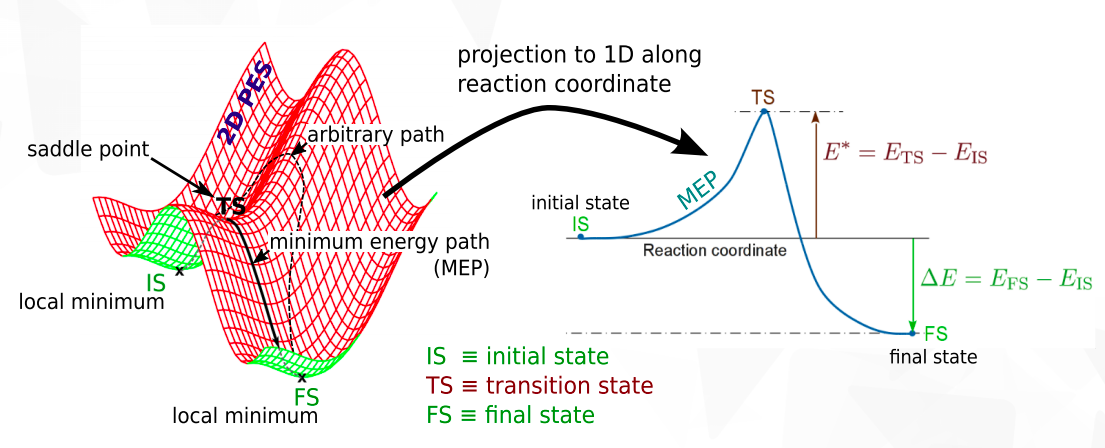
\includegraphics[scale = 0.4]{figs/D3/saddle.png}
      \caption{Proyección bidimensinal de una PES marcando sus puntos más importantes. Tomando el MEP se puede hacer una proyección unidimensional.}
      \label{fig:saddle}
  \end{figure}

  La importancia de la energía de activación radica en que es un muy buen criterio para decidir si cierto proceso activado es cinéticamente posible a cierta temperatura y, de serlo, qué tan rápido es. La constante de velocidad es
    $$k = \nu \exp(-E^{*} \beta) \quad ; \quad \nu = \frac{\prod_{j=1}^{3N} \nu_j^{IS} }{\prod_{j=1}^{3N-1} \nu_j^{TS}}$$

  Aunque típicamente $\nu \approx 10^{13} s^{-1}$, en realidad depende del tipo de proceso: para la desorción suele ser $\nu \approx 10^{16} s^{-1}$ por ejemplo (ver Surf. Sci. Rep. 12, 183-242 (1991)).

  En el contexto del análisis de procesos activados, se conoce como \emph{imagen} a una dada configuración del sistema completo. Vamos a usar además un vector $\vec{R}$ que representa en realidad al vector $3N$ dimensional con todas las coordenadas de los $N$ núcleos. Así $\vec{R}^{(n)}$ es el vector posición de los $N$ núcleos en la $n$-ésima iteración.

\subsection{NEB}

  El estado inicial y el final son mínimos, por lo que deben encontrase mediante métodos de optimización. Por otro lado, encontrar el saddle es bastante más complicado. Un método para encontrarle es el NEB (Nudged Elastic Band). La idea es la siguiente (Fig. \ref{fig:NEB}):
    \begin{enumerate}
      \item Conectamos el estado inicial y el final con una \emph{banda elástica}, la cual es tan elástica como sea necesario, \emph{i.e.} no se puede cortar nunca.
      \item Relajamos la bandita mediante fuerzas ortogonales ($\vec{F}_{\perp}$) a la misma.
      \item Eventualmente se alcanaz $\vec{F}_{\perp} = 0$. La bandita resultante marca el MEP y determina el saddle.
    \end{enumerate}

    \begin{figure}[H]
        \centering
        \subfigure[]{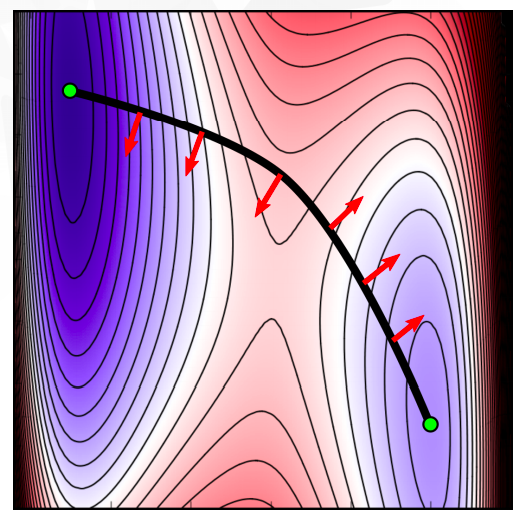
\includegraphics[scale = 0.30]{figs/D3/NEB_2a.png}}
        \subfigure[]{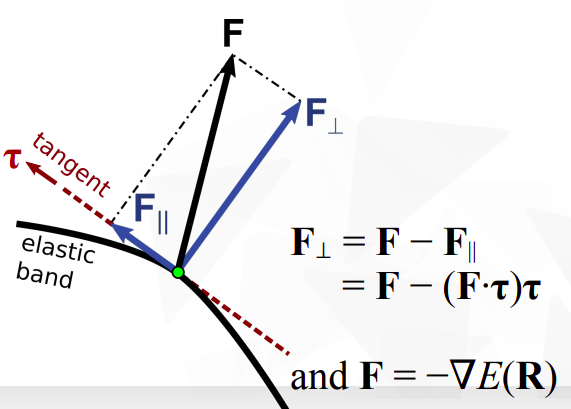
\includegraphics[scale = 0.25]{figs/D3/NEB_2b.png}}
        \subfigure[]{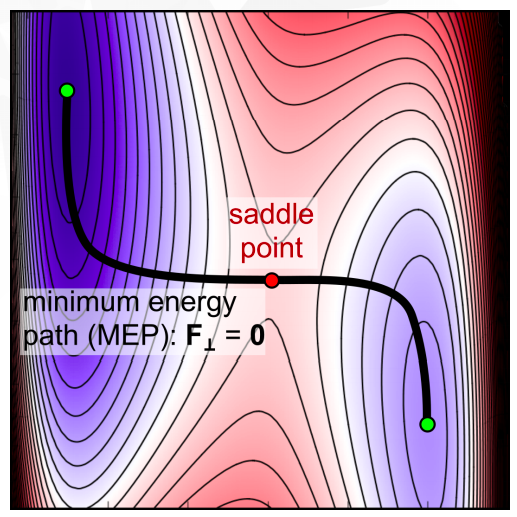
\includegraphics[scale = 0.30]{figs/D3/NEB_2c.png}}
        \caption{(a) Cómo conectamos el estado inicial con el final en NEB: la línea negra representa la banda elástica, mientras que las flechas rojas son las contribuciones ortogonales de la fuerza. (b) Descomposición de la fuerza aplicada sobre la bandita. (c) Resultado final donde $\vec{F}_{\perp} = 0$: la bandita marca el MEP.}
        \label{fig:NEB}
    \end{figure}

  Computacionalmente necesitamos discretizar la bandita elástica en una cantidad finita de imágenes: la fuerza perpendicular es calculada sobre estas imágenes. El problema de la discretización es que no preserva la distancia entre imágenes, lo cual puede dar lugar a distintos problemas a medida que avanzan las iteraciones. Para solucionar este problema, las imágenes son conectadas mediante resortes (Fig. \ref{fig:disc}), los cuales sólo actuan a lo largo del camino de reacción para mantener la distancia inter-imágenes.

  \begin{figure}[H]
      \centering
      \subfigure[]{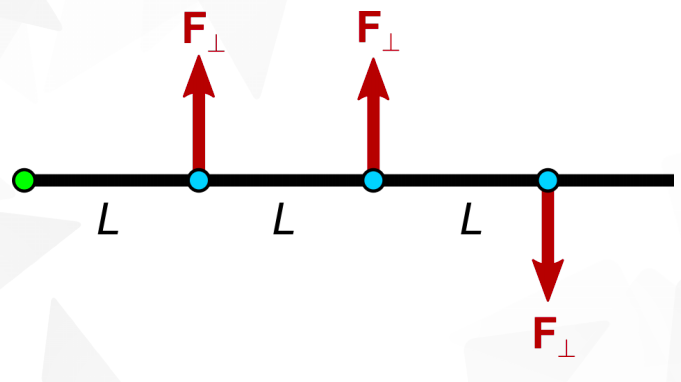
\includegraphics[scale = 0.3]{figs/D3/disc_a.png}}
      \subfigure[]{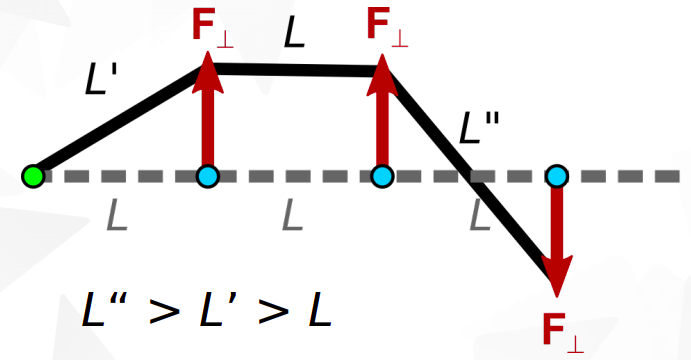
\includegraphics[scale = 0.3]{figs/D3/disc_b.png}}
      \subfigure[]{\includegraphics[scale = 0.35]{figs/D3/disc_c.png}}
      \caption{Al discretizar (a) las fuerzas pueden provocar que el camino entre imágenes no se conserve (b). Esto se soluciona utilizando resortes (c).}
      \label{fig:disc}
  \end{figure}

  Reuniendo toda la info rmación nos queda entonces que NEB consiste en (Fig. \ref{fig:NEB_disc}):
    \begin{enumerate}
      \item Conectar dos mínimos con un camino de reacción. Esto debe proponerse, pudiendo ser simplemente una interpolación lineal (default).
      \item Discretizar el camino de reacción mediante imágenes ($\left\{ \vec{R}_j \right\}_{j=1}^M$).
      \item Conectar las imágenes con resortes.
      \item Minimizar el camino de reacción mediante NEB: sobre la $j$-ésima imagen se aplica una fuerza perpendicular a la banda, moviéndola, y una tangencial que es la del resorte. Estos son los \emph{empujones} (nudgings) que dan lugar al nomnbre.
    \end{enumerate}

  \begin{figure}[H]
      \centering
      \includegraphics[scale = 0.4]{figs/D3/disc_a.png}
      \caption{NEB considerando discretización y resortes.}
      \label{fig:NEB_disc}
  \end{figure}

  La elección de la tangente es crucial para la convergencia. Una buena elección es considerar una tangente local, la cual sólo considera la imagen adyacente de mayor energía. En caso de que la imagen tenga menor energía que ambas imágenes adyacentes se toma un promedio.

  Como el interés está centrado en conocer el saddle, debemos aumentar la resolución de la zona. Para ello podemos usar constantes del resorte variables entre dos valores dados. Cuanto mayor sea la energía de la imagen, más rígido debe ser el resorte. Así la densidad de imágenes en la proximidad del saddle será mayor.

  En QE se pueden utilizar imágenes intermedias que permiten dar una guía para el camino de reacción inicial (Fig. \ref{fig:inter}). Muy útil cuando se tiene una intuición de la situación. Sólo son una guía, pero no se toman como imágnees para el cálculo.

  \begin{figure}[H]
      \centering
      \includegraphics[scale = 0.4]{figs/D3/inter.png}
      \caption{Uso de imágenes intermedias.}
      \label{fig:inter}
  \end{figure}

\subsubsection{CI-NEB}

  Incluso cuando se tienen muchas imágenes y constantes de resorte variables, puede ocurrir que ninguna imagen quede lo suficientemente cerca del estado del saddle. Una solución al problema es recurrir al Climbing Image NEB (CI-NEB), donde se le permite a la imagen de mayor energía \emph{escalar} al desacoplarle los resortes. Para escalar necesitamos invertir la fuerza tangcial sobre la banda.

  \begin{figure}[H]
      \centering
      \includegraphics[scale = 0.4]{figs/D3/climb.png}
      \caption{Uso de imágenes intermedias en CI-NEB.}
      \label{fig:climb}
  \end{figure}

\subsection{neb.x}

  Se tienen dos bloques en el input: el primero contiene las especificaciones para NEB, mientras que en el segundo están las especificaciones para pw.x. En la parte del NEB tenemos una sección obligatoria donde definimos el camino de reacción y una parte opcional si queremos hacer CI-NEB (Figs. \ref{fig:nebx} y \ref{fig:nebx_2}). En la parte del PW tenemos que poner más cosas en la carta de posiciones (Fig. \ref{fig:pwx}).

  \begin{figure}[H]
      \centering
      \includegraphics[scale = 0.4]{figs/D3/nebx.png}
      \caption{Input file: neb part.}
      \label{fig:nebx}
  \end{figure}

  \begin{figure}[H]
      \centering
      \includegraphics[scale = 0.4]{figs/D3/nebx_2.png}
      \caption{Input file: neb part con más detalles.}
      \label{fig:nebx_2}
  \end{figure}

  \begin{figure}[H]
      \centering
      \includegraphics[scale = 0.4]{figs/D3/pwx.png}
      \caption{Input file: pw part.}
      \label{fig:pwx}
  \end{figure}

  Si usamos $use\_freezing = .true.$ el cálculo primero movera aquellas imágenes que tengan mayor error según algún criterio. Esto es conveniente: es mejor primero optimizar sólo aquellas imágenes de mayor error respecto al mínimo de energía (Fig. \ref{fig:nebxout}).

  \begin{figure}[H]
      \centering
      \includegraphics[scale = 0.5]{figs/D3/nebxout.png}
      \caption{Output file.}
      \label{fig:nebxout}
  \end{figure}

\subsection{Aspectos generales de NEB}

  Los cálculos NEB suelen tener una convergencia difícil. Por lo tanto es conveniente:
    \begin{itemize}
      \item Usar la experiencia es relevante: usar intuición química.
      \item Usar estados inicial y final ya relajados. En este sentido, no conviene utilizar $first\_last\_opt = .true.$.
      \item Usar imaǵenes intermedias.
    \end{itemize}

  La cantidad de imágenes a utilizar es variable. Una distancia entre imágenes de 1 ó 2 Bohr suele ser suficiente. Esta distancia se imprime en el output por lo que se recomiendo hacer un dryrun haciendo $nstep_path = 0$ (Fig. \ref{fig:dryrun}).

  \begin{figure}[H]
      \centering
      \includegraphics[scale = 0.7]{figs/D3/dryrun.png}
      \caption{Dryrun para conocer la distancia entre imágenes.}
      \label{fig:dryrun}
  \end{figure}

  Es bueno visualizar previamente el camino de reacción inicial antes de hacer el cálculo. Esto se puede hacer con xcrysden:
    $$xcrysden \quad --pwi \quad neb.in$$

  Es conveniente calcular un paso elemental a la vez (una única saddle). La opción $CI\_scheme = 'manual'$ permite calcular varios saddle en simultáneo.

  Usar $use\_freezing = .true.$ suele ser beneficioso.

  Respecto a los valores de las constantes de resorte mínima y máxima, no son tan importantes para el cálculo: el default suele funcionar bien. De lo contrario, en el output el programa sugiere valores.

  No es conveniente activar CI-NEB desde el comienzo. Primero debemos relajar el camino de reacción para lograr la mayor estabilidad posible. Recién ahí activamos el CI-NEB ($CI\_scheme = 'auto'$). Esto es porque a medida que avanzan las iteraciones puede ir cambiando qué imagen es la de mayor energía, dando lugar a oscilaciones. Esto se puede setear e PWTK (Fig. ).

  \begin{figure}[H]
      \centering
      \includegraphics[scale = 0.8]{figs/D3/PWTK.png}
      \caption{Cómo escribir en PWTK para tener CI-NEB apagado al comienzo y luego encenderlo.}
      \label{fig:PWTK}
  \end{figure}

  No deben intercambiarse las posiciones (los índices) de los átomos en el input: las inconsistencias se rompe el programa.

  You cannot do:
  xcrysden --pwo neb.out
  Why? Look into the neb.out output file and you will notice there are no atomic coordinates there.
  Instead, neb.x writes a number of prefix.* files, in particular:
  prefix.dat -- energies of images
  prefix.int -- interpolated energies on a denser grid (larger number of images)
  prefix.axsf -- xcrysden XSF file for visualization
  etc.
  Hence you can do: xcrysden --xsf prefix.axsf
  Where prefix is as set in the input (e.g. H2+H, ...). Do "ls" and you will notice these files.

\section{Q\&A 2/2}

\definicion{I have heard that doing a CI-NEB calculation is not enough to assert that the saddle point found is the transition state. In addition to that, a phonon calculation must be done. The obtained state can be considered as the transition state only if we obtain imaginary frequencies. Is that true ?}

In general yes, however the CI-NEB should get you close enough for all practical purposes, at least for systems that you can't afford a phonon calculation

\definicion{How chemisorbtion is different from physiorbtion in qe and how they are performed}

Short answer: QE doesn't care, it calculates from first principles.
Note however that dispersion interactions are not described by plain DFT functionals, hence you need to use some special functional or a semi-empiric dispersion correction: you will learn that tomorrow.

\definicion{In order to have the best IS and FS in neb calculations can we perform a preliminar 'relax' or 'vc-relax' calculations of both the IS and the FS and then use the structural optimized parameters to perform the neb calculation? Or there are other ways to do that?}

Yes, this is my recommendation, i.e. optimize the first and the last image, then make intermediate images (if needed) and only then do NEB calc.
I am not sure vc-relax NEB is implemented in QE (I have never used it)

\definicion{we have to keep the same lattice parameters in both IS and FS? right?}

Yes. In the input on neb, you have to enter the common lattice parameter.

\section{Hands-on}

\definicion{Topic:} Optimizations, NEB. Automating the workflow (PWTK).

\definicion{Speaker:} Ari Paavo SEITSONEN (École Normale Supérieure, Paris).

\subsection{relax}

\subsubsection{Objetivo}

  Realizar una optimización estructural de las posiciones atómicas, tanto con grafeno como con óxido de grafeno.

\subsubsection{Pasos}

  Para el caso del grafano (grafeno con un H en cada C en trans):

    \begin{enumerate}
      \item Notar que en el input ahora hay una nueva namelist: \&IONS. Correr con
        \begin{verbatim}
          pw.x -in pw.graphane.relax.in > pw.graphane.relax.out &
        \end{verbatim}
      \item Analizar el output: son sucesivos pasos de SCF seguidos de cálculos de fuerzas para determinar las nuevas posiciones atómicas.
      \item visualizar la evolución estructural.
        \begin{verbatim}
          xcrysden --pwo pw.graphane.relax.out
        \end{verbatim}
    \end{enumerate}

  Para el óxido de grafeno (átomo de grafeno adsorbido sobre una celda 3x3 de grafeno) hacer lo mismo: hacer la relajación y luego visualizarla.

    \begin{verbatim}
      pw.x -in pw.graphene3x3-O.relax.in > pw.graphene3x3-O.relax.out &
      xcrysden --pwo pw.graphane.relax.out
    \end{verbatim}

\subsubsection{Resultados: relax}

  Primero analizamos el grafano. En 5 ciclos SCF converge:

    !    total energy              =     -24.78069777 Ry
         estimated scf accuracy    <          1.4E-09 Ry
    !    total energy              =     -25.01952054 Ry
         estimated scf accuracy    <          2.0E-09 Ry
    !    total energy              =     -25.10918098 Ry
         estimated scf accuracy    <          6.3E-09 Ry
    !    total energy              =     -25.11219615 Ry
         estimated scf accuracy    <          1.2E-09 Ry
    !    total energy              =     -25.11408866 Ry
         estimated scf accuracy    <          9.5E-11 Ry
    !    total energy              =     -25.11411542 Ry
         estimated scf accuracy    <          2.6E-10 Ry

  A partir de la figura vemos que se acomoda en su disposición tetraédrica dada la hibridización sp3. Se peude ver que la saturación provoca que pierda parte de sus propiedades eléctricas. Por eso todo lo respecto al smearing está comentado en el input.

  \begin{figure}[H]
      \centering
       \subfigure[]{\includegraphics[scale = 0.30]{figs/D3/Grafano_in.png}}
       \subfigure[]{\includegraphics[scale = 0.30]{figs/D3/Grafano_out.png}}
       \caption{Grafano antes (a) y después (b) de la relajación.}
   \end{figure}

  Después tenemos un expoxi- sobre una superficie de grafeno en una cupercelda (es 3x3 pero también debería estudairse este tamaño medainte test de convergencia). En este caso sí usamos ocupación fraccionaria (smearing). Debería usarse una $k$-mesh de 3x3x3, pero se usó gamma para que sea más rápido. La distancia entre átomos de carbono es mayor para los que participan del epóxido respecto a los demás carbonos del grafeno. Esto se puede asociar a hibridización de cada uno de los C.

  \begin{figure}[H]
      \centering
       \subfigure[]{\includegraphics[scale = 0.30]{figs/D3/GrO_relax_in.png}}
       \subfigure[]{\includegraphics[scale = 0.30]{figs/D3/GrO_relax_out.png}}
       \caption{Grafeno oxidado con un grupo epoxi antes (a) y después (b) de la relajación.}
   \end{figure}

  \Obs{Como tenemos 2 átomos diferentes, deberíamos haber chequeado la convergencia de los cutoffs para ambos elementos y tomar el valor más alto.}

\subsection{vc-relax}

\subsubsection{Objetivo}

  Realizar un cálculo de optimización estructural, relajando también los parámetros de red.

\subsubsection{Pasos}

  Primero se analiza Zn bulk:
    \begin{enumerate}
      \item Analizar los cambios en el input y correr
        \begin{verbatim}
          pw.x -in pw.Zn.vc-relax.in > pw.Zn.vc-relax.out &
        \end{verbatim}
      \item Analizar el output: ciclos SCF, fuerzas y tensores de estrés llevan a nuevos parámetros de red y posiciones atómicas.
      \item Visualizar.
      \begin{verbatim}
        xcrysden --pwo pw.Zn.vc-relax.out
      \end{verbatim}
    \end{enumerate}

  Una alternativa es hacer un barrido bidimensional de ambos parámetros de red con
    \begin{verbatim}
      pwtk Zn-scan.pwtk
    \end{verbatim}

  La PES resultante se puede ver con
    \begin{verbatim}
      gnuplot plot2D.gp
    \end{verbatim}

  Luego se analiza un cristal molecular de urea:
    \begin{enumerate}
      \item Ejecutar
      \begin{verbatim}
        pw.x -in pw.urea.vc-relax.in > pw.urea.vc-relax.out &
      \end{verbatim}
    \end{enumerate}

  \Obs{Estos cálculos ya son bastante más pesados así que conviene mandarlos al cluster.}

\subsubsection{Resultados: vc-relax}

  Empezamos con el cluster de Zn. Primero hacemos una relajación con un par de CI fijas: el programa buscará el mínimo. Vemos que la celda se agranda:
    $$celldm(1) =  4.8 \Rightarrow celldm(1) = 4.96 \Rightarrow a = 2.62\ \si{\angstrom}$$
    $$celldm(3) =  1.8 \Rightarrow celldm(3) = 2.02 \Rightarrow c = 5.29\ \si{\angstrom}$$

  \begin{figure}[H]
      \centering
       \subfigure[]{\includegraphics[scale = 0.30]{figs/D3/Zn_vc_in.png}}
       \subfigure[]{\includegraphics[scale = 0.30]{figs/D3/Zn_vc_out.png}}
       \caption{Bulk de Zn antes (a) y después (b) de la relajación tanto de posiciones atómicas como de parámetros de red.}
   \end{figure}

  \Obs{El orden de qué tan fácil es alcanzar la convergencia es: energías, fuerzas y estrés. A medida que avanzamos en dificultad, necesitamos cutoffs más altos.}

  La segunda opción es hacer un barrido bidimensional. En este caso no hacemos una vc-relax, sino que por cada par de CI hacemos una SCF. Aunque esto no da un valor tan exacto como el vc-relax, permite conocer la región donde se encuentra el mínimo. Luego puedo hacer una interpolación para hallar el mínimo o hacer un vc-relax pero dando CI cercanas al mínimo.

  Si vemos el mapa, podemos reconocer que el mínimo está aproximadamente en $a = 2.6\ \si{\angstrom}$ y $c = 5.2\ \si{\angstrom}$. Esto está bastante cerca de los valores calculados mediante vc-relax.

  \begin{figure}[H]
      \centering
       \includegraphics[scale = 0.30]{figs/D3/Zn_scan.png}
       \caption{Análisis bidimensional de los parámetros de red para el Zn bulk.}
   \end{figure}

  \Obs{En general ocurre que los parámetros de red calculados no coinciden completamente con los experimentales incluso habiendo elegido los valores que minimizan los errores, \emph{i.e.} habiendo estudiado la convergencia. Esto se debe al término de XC. Conviene usar los valores de nuestra convergencia para hacer los estudios: así los cálculos posteriores tendrán minimizadas sus fuentes de error.}

  En el caso de la urea tamibién se ve que la celda se agranda, pero el cambio es más sutil.

  \begin{figure}[H]
      \centering
       \subfigure[]{\includegraphics[scale = 0.30]{figs/D3/urea_vc_in.png}}
       \subfigure[]{\includegraphics[scale = 0.30]{figs/D3/urea_vc_out.png}}
       \caption{Urea antes (a) y después (b) de la relajación tanto de posiciones atómicas como de parámetros de red.}
   \end{figure}

\subsection{NEB: transferencia de H}

\subsubsection{Objetivo}

  Hacer una búsqueda del estado de transición para una reacción química simple utilizando el método NEB (neb.x).

\subsubsection{Pasos}

  En el primero ejemplo tenemos una transferencia de protones: H + H2 --> H2 + H. Primero no utilizamos una imagen intermedia:

    \begin{enumerate}
      \item Solo se dan las imágenes inicial y final y neb.x hace una interpolación lineal con la cantida de imágenes deseadas. El camino de reacción inicial se puede visualziar con
        \begin{verbatim}
          xcrysden --pwi neb.H2+H.in
        \end{verbatim}
      \item Correr el programa.
      \begin{verbatim}
        neb.x -in neb.H2+H.in > neb.H2+H.out
      \end{verbatim}
      \item Analizar el output. ¿Cuántos pasos fueron necesarios para la convergencias? ¿Cuánto vale la barrera de activación?
      \item Plotear el MEP.
      \begin{verbatim}
        gnuplot H2+H.gp
      \end{verbatim}
      \item Visualizar las estructuras del MEP con alguno de los siguientes comandos.
      \begin{verbatim}
        xcrysden --xyz H2+H.xyz
        xcrysden --axsf H2+H.axsf
      \end{verbatim}
    \end{enumerate}

  Luego usamos una imagen intermedia:
    \begin{enumerate}
      \item Visualizar el camino inicial. Comparar con el caso anterior.
        \begin{verbatim}
          xcrysden --pwi neb.H2+H.w-inter-image.in
        \end{verbatim}
      \item Correr el programa.
      \begin{verbatim}
        neb.x -in neb.H2+H.w-inter-image.in > neb.H2+H.w-inter-image.out &
      \end{verbatim}
      \item Analizar el output. Comparar barreras de activación
    \end{enumerate}

    \begin{figure}[H]
        \centering
          \includegraphics[scale = 0.6]{figs/D3/imagen_intermedia.png}
         \caption{Comparación entre no usar (a) y usar (b) imagen intermedia.}
     \end{figure}

\subsubsection{Resultados: transferencia de H}

  La reacción es una transferencia de protones. En el primer ejemplo no utilizamos imágnes intermedias: sólo especificamos la primera imágen (reactivos) y la última (productos). El camino de reacción se discretiza en 7 imágenes y neb.x hace una interpolación lineal para ubicar las faltantes. El segundo ejemplo aprovecha un poco de intuición química para intentar dar un mejor camino de reacción inicial. Dada la ayuda que le damos al programa, la convergencia se alcanzará en menos pasos.

  \Obs{El umbral de convergencia $path\_thr = 0.1$ no es el óptimo, sino que se eligió para que corriera más rápido.}

  \begin{figure}[H]
      \centering
       \subfigure[]{\includegraphics[scale = 0.30]{figs/D3/NEB_H3_noint_in.png}}
       \subfigure[]{\includegraphics[scale = 0.30]{figs/D3/NEB_H3_int.png}}
       \subfigure[]{\includegraphics[scale = 0.30]{figs/D3/NEB_H3_noint_out.png}}
       \caption{Transferencia de protones: punto inicial (a) y final (c) de la reacción. En (b) se tiene la imagen intermedia considerada.}
   \end{figure}

  La corrida con imagen intermedia terminó en unos 5 minutos, mientras que la otra ya va más de 45 minutos. Sus perfiles son iguales: la simetría es porque en reactivos y productos tenemos exactamente lo mismo. Sin embargo, se ve que la corrida sin imagen itnermedia alcanza una barrera de activación mayor: sin imagen itnermedia se llega a 0.2844 eV, mientras que con imagen intermedia tenemos 0.2690 eV. De todas formas la diferencia no es significativa, poniendo en relevancia que es mejor hacer el cálculo con imagen intermedia.

  \begin{figure}[H]
      \centering
       \subfigure[]{\includegraphics[scale = 0.45]{figs/D3/NEB_H3_L.png}}
       \subfigure[]{\includegraphics[scale = 0.45]{figs/D3/NEB_H3_C.png}}
       \caption{Perfil de reacción sin (a) y con (b) iamgen intermedia.}
   \end{figure}

\subsection{NEB: disociación de H}

\subsubsection{Objetivo}

   Llevar a cabo una NEB no trivial.

\subsubsection{Pasos}

  No sólo usaremos imágenes intermedias, sino que además dividiremos el cálculo NEB en dos etapas para así ayudar a la convergencia ya que haremos CI-NEB: primero haremos una NEB común ($CI\_scheme = 'no-CI'$) para estabilizar un poco el camino de reacción y, luego, permitimos que escale ($CI\_scheme = 'auto'$). Esto es más fácil de hacer usando PWTK. En la primera etapa el umbral de convergencia es mayor.

       \begin{enumerate}
         \item Visualizar el camino de reacción inicial.
           \begin{verbatim}
             xcrysden --pwi neb.H2-diss.Al100-2x1-2L.in
           \end{verbatim}
          \item Correr el programa.
          \begin{verbatim}
            remote_pwtk neb.pwtk
          \end{verbatim}
          \item Cuando termina, traer los resultados.
          \begin{verbatim}
            rsync_from_hpc '*.out'
          \end{verbatim}
          \item Analizar resultados. ¿Cuántos pasos necesito la convergencia? ¿Cuál es la barrera de activación?
          \item Graficar el MEP.
          \begin{verbatim}
            gnuplot H2-diss.Al100-2x1-2L.gp
          \end{verbatim}
          \item Visualizar los cambios estructurales.
          \begin{verbatim}
            xcrysden --axsf H2-diss.Al100-2x1-2L.axsf
          \end{verbatim}
       \end{enumerate}

\subsubsection{Resultados: disociación de H}

  Tenemos la disociación de hidrógeno molecular sobre AL(100).

  \begin{figure}[H]
      \centering
       \subfigure[]{\includegraphics[scale = 0.30]{figs/D3/diss_ini.png}}
       \subfigure[]{\includegraphics[scale = 0.30]{figs/D3/diss_inter.png}}
       \subfigure[]{\includegraphics[scale = 0.30]{figs/D3/diss_fin.png}}
       \caption{Disociación de hidrógeno molecular sobre AL(100): punto inicial (a) y final (c) de la reacción. En (b) se tiene la imagen intermedia considerada.}
   \end{figure}

  Se puede ver que la barrera de activación es de 1.17 eV. La asimetría de la curva es porque los productos son más estables que los reactivos.

   \begin{figure}[H]
       \centering
        \includegraphics[scale = 0.45]{figs/D3/diss.png}
        \caption{Perfil de reacción para la disociación de hidrógeno molecular sobre AL(100).}
    \end{figure}

\subsection{pwtk automation}

\subsubsection{Objetivo}

  Se hacen diferentes pruebas con el fin de explorar las capacidades de PWTK:
    \begin{enumerate}
      \item Cómo usar EOS (Equation of State) utility de PWTK: calcular EOS de Rh bulk.
      \item Cómo correr varios cálculos con un script PWTK simple: calcular la PES bidimensional de las posiciones laterales de O @ Al(111).
      \item Cómo ensamblar varios cálculos con PWTK: analizar enlace de CO sobre Rh(100).
    \end{enumerate}

    \Obs{Los parámetros son pobres con el fin de acelerar la convergencia. Todos los ejemplos importan el archivo common.pwtk donde se especifican el conjunto común da input data utilizado en todos los ejemplos: PP, cutoffs, smearing, etcétera.}

\subsubsection{Pasos: EOS}

  Para calcular la EOS de un sistema cúbico usando la EOS utility de PWTK:

  \begin{enumerate}
    \item Ejecutar
      \begin{verbatim}
        pwtk eos.Rh-bulk.pwtk > eos.Rh-bulk.log &
      \end{verbatim}
    \item Leer el archivo de salida 'eos.Rh-bulk.log'. Los resultados finales están en 'eos.Rh-bulk.RESULTS'.
  \end{enumerate}

\subsubsection{Resultados: EOS}

  Lo que estamos corriendo permite encontrar los valores óptimos del parámetro de red para sistemas cúbicos o hcp. Se hacen 15 cálculos del tipo sCF con diferentes parámetros de red. Usa una guess inicial como input y estos resultados son el input de ev.x para calcular la EOS.

  Notamos que el módulo de Young es más sensible al muestreo de datos que al parámetro de red y la energía de equilibrio total.

  \begin{figure}[H]
      \centering
      \subfigure[]{\includegraphics[scale = 0.35]{figs/D3/eos_etot.png}}
      \subfigure[]{\includegraphics[scale = 0.35]{figs/D3/eos_alat.png}}
      \subfigure[]{\includegraphics[scale = 0.35]{figs/D3/eos_young.png}}
      \caption{Resultado de EOS en Rh bulk.}
  \end{figure}

\subsubsection{Pasos: O@Al(111)}

  Mediante el estudio de una PES bidimensional se pretende introducir el conecpt de input data stacking en PWTK (input\_pushpop { ... }).
  \begin{enumerate}
    \item Ejecutar.
      \begin{verbatim}
        remote_pwtk scan.pwtk
      \end{verbatim}
    \item Ver la PES resultante.
    \begin{verbatim}
      gnuplot plot2D.gp
    \end{verbatim}
    \item Ejecutar tabulation para plotear automáticamente las estructuras de los outputs de las diferentes pw.x. Esto genera un archivo (tabulate.tex)
    \begin{verbatim}
      pwtk tabulate.pwtk
      pdflatex tabulate.tex
    \end{verbatim}
  \end{enumerate}

\subsubsection{Resultados: O@Al(111)}

  En cada iteración deberíamos agregar un nuevo átomo de oxígeno a la estructura. Sin embargo, al usar input data stacking, agregamos un oxígeno, hacemos el cálculo y luego quitamos dicho O. Dicho O queda fijo en su posición en el plano,  pero tiene libertad para moverse en $z$.

  El concepto de input data stacking sirve cuando se hacen múltiples cálculos que poseen un set de parámetros en común y debemos ir haciendo pequeñas modificaciones, pero no secuenciales: cada corrida debe ser independiente del estado final de la corrida anterior. Para lograr esto se usa $inpu\_push$ y $inpu\_pop$ (o directametne $inpu\_pushpop$).

  \begin{figure}[H]
      \centering
      \includegraphics[scale = 0.4]{figs/D3/pushpop.png}
  \end{figure}


    \begin{figure}[H]
        \centering
        \includegraphics[scale = 0.45]{figs/D3/PES_2D.png}
        \caption{PES 2D para O@Al(111).}
    \end{figure}

  El resultado de la tabuación se puede ver en la siguiente figura.

  \begin{figure}[H]
      \centering
      \includegraphics[scale = 0.7]{figs/D3/tabulate.png}
      \caption{Ubicación de O respecto a la superficie de Al(111).}
  \end{figure}

\subsubsection{Pasos: CO@Rh(100)}

  \begin{enumerate}
    \item Ejecutar todo. Necesitamos 8 procesadores ya que una de las etapas es calcular la molécula de CO aislada y con más procesadores se crashea.
      \begin{verbatim}
        NPROC=8 remote_pwtk run-all.pwtk
      \end{verbatim}
    \item Traer lo relevante.
    \begin{verbatim}
      rsync_from_hpc *.in *.out *.xsf *pdos*
    \end{verbatim}
  \end{enumerate}

  Para visualizar todo:
    \begin{enumerate}
      \item Ver PDOS y MOPDOS. Setear antes la energía de Fermi en $moproj.gp$.
      \begin{verbatim}
        grep Fermi pw.CO-Rh100.nscf.out
        gnuplot moproj.gp
      \end{verbatim}
      \item Los MO se escriben en $psi2.CO_K*_B*.xsf$. Verlos de a uno o todos juntos.
      \begin{verbatim}
        xcrysden -r 0 --xsf psi2.CO_K001_B005.xsf
        ./plot-psi2.sh
      \end{verbatim}
      \item Los ILDOS estan en $ildos_*.xsf$. Verlos de a uno o todos juntos.
      \begin{verbatim}
        xcrysden -r 2 --xsf ildos_-3.05_-2.95.xsf
        ./plot-ildos.sh
      \end{verbatim}
      \item La DIFDEN está en $difden.CO-Rh100.xsf$. Ver con
      \begin{verbatim}
        xcrysden -r 2 --xsf difden.CO-Rh100.xsf
      \end{verbatim}
    \end{enumerate}

\subsubsection{Resultados: CO@Rh(100)}

  Vamos a analizar el enlace de CO sobre Rh(100) mediante varias técnicas: charge-density difference (DIFDEN), density-of-states projected (PDOS) to atomic orbitals, density-of-states projected to molecular orbitals (MOPDOS) y ILDOS (integrated-local density of states).

  Los scripts son:
    \begin{itemize}
      \item \textbf{common-data.pwtk:} input data común a todos los cálculos.
      \item \textbf{run-all.pwtk:} importa los demás scripts y hace los cálculos.
      \item \textbf{relax.pwtk:} relajación de la estrucutura de Co-Rh(100).
      \item \textbf{difden.pwtk:} calculo de la diferencia de densidad de carga. Esta es una utility de PWTk que ayuda a hacer cálculos de diferencias, no sólo la de densidad de carga. En el caso particular que buscamos para resolver $\Delta\rho_{AB} = \rho_{AB} - \rho_A - \rho_B$ necesitamos 7 cálculos: una SCF (pw.x) y una densida de carga (pp.x) para AB, A y B más un pp.x extra que hace la diferencia. Este script lleva a cabo todos los 7 cálculos.
      \item \textbf{ildos.pwtk:} calculo de la ILDOS.
      \begin{figure}[H]
          \centering
          \subfigure[]{\includegraphics[scale = 0.7]{figs/D3/ILDOS.png}}
          \subfigure[]{\includegraphics[scale = 0.7]{figs/D3/ILDOSs.png}}
          \caption{Representación de ILDOS.}
      \end{figure}
      \item \textbf{pdos.pwtk:} cálculo de la PDOS y la MOPDOS. Además plotear los MO de Co.
    \end{itemize}

    \begin{figure}[H]
        \centering
        \includegraphics[scale = 0.7]{figs/D3/CO_DOS.png}
        \caption{PDOS y MOPDOS.}
    \end{figure}

    \begin{figure}[H]
        \centering
        \includegraphics[scale = 0.2]{figs/D3/psi2-montage.png}
        \caption{MO de CO.}
    \end{figure}

    \begin{figure}[H]
        \centering
        \includegraphics[scale = 0.2]{figs/D3/ildos-montage.png}
        \caption{ILDOS.}
    \end{figure}

    \begin{figure}[H]
        \centering
        \includegraphics[scale = 0.7]{figs/D3/CO_DIFDEN.png}
        \caption{ILDOS.}
    \end{figure}

    Se observa la donación de carga del $\sigma$-HOMO del CO a los estados metálicos y, luego, la donación vuelve hacia el $\pi^*$-LUMO del CO.


    \chapter{Día 4}

      \section{Teórico}

  \definicion{Topic:} Advanced functionals: higher accuracy (hybrids), strongly correlated materials (DFT+U), weakly bound systems (van der Waals).

  \definicion{Speaker:} Stefano DE GIRONCOLI (SISSA, Italy).

\subsection{Funcionales en DFT: término XC}

  Existen diferencias generaciones o grupos de funcionales que van creciendo en precisión, pero esto conlleva un incremento en su complejidad (Fig. \ref{fig:jacob}): incluso el funcional más sencillo contiene información acerca de la densidad de carga del sistema.

  \begin{figure}[H]
      \centering
      \includegraphics[scale = 0.5]{figs/D4/Jacob.png}
      \caption{Escalera de Jacob de las aproximaciones de DFT.}
      \label{fig:jacob}
  \end{figure}

  Los teoremas de Hohenberg-Kohn (HK) están relacionados a cualquier sistema que consista de electrones moviéndose bajo la influencia de un potencial externo:
    \begin{enumerate}
      \item \textbf{Primer teorema HK:} el potencial externo y, en consecuencia, la energía total son un funcional único de la densidad electrónica. Luego, la densidad electrónica del estado fundamental describe de manera unívoca el potencial y, por lo tanto, todas las propiedades del sistema, incluyendo la función de onda many-body. Se sigue que el espectro del Hamiltoniano también es un funcional único de dicha densidad basal. Particularmente, el funcional HK es una función universal de la densidad electrónica, no dependiendo de manera explícita del potencial externo.
        $$F[n] = T[n] + U[n]$$
      \item \textbf{Segundo teorema HK:} El funcional permite determinar la energía del estado fundamental si y sólo si la densidad electrónica es la del estado fundamental.
        $$F [n] = \underbrace{min}_{\Psi \rightarrow n} \bra{\Psi} T_e + W_{ee} \ket{\Psi}$$
    \end{enumerate}

  Se tiene entonces que para cualquier natural $N$ y potencial externo $v_{ext} (\vec{r})$ existe un funcional de desidad $F[n]$ tal que
    $$E [n] = F[n] + \int v_{ext} (\vec{r}) n (\vec{r}) d\vec{r}$$

  Partiendo de esta idea, KS plantean la energía cinética de un sistema ficticio de electrones no interactuantes.
    $$T_s[n] = \underbrace{min}_{\Psi \rightarrow n} \bra{\Psi} T_e\ket{\Psi}$$

  Con esta información se reescribe la ecuación de HK según del sistema interactuante según
    $$F[n] = T_s[n] + E_{Har} [n] + E_{XC} [n]$$

  Así la energía del sistema será
    $$E [n] = T_s[n] + E_{Har} [n] + E_{XC} [n] + \int v_{ext} (\vec{r}) n (\vec{r}) d\vec{r}$$

  Todo lo que quedó fuera al recurrir a este sistema no interactuante está contenido en el término XC. Este término es pequeño relativo a los demás términos que contribuyen a la energía total del sistema. Por este motivo es que incluso la aproximación más sencilla sigue siendo útil para los cálculos.

\subsection{L(S)DA}

  La aproximación más sencilla es Local (Spin) Density Approximation (L(S)DA), donde la "S" se pone según se esté considerando o no la contribución de spin. En este caso basta con conocer la densidad electrónica en cada punto del espacio.
    $$E_{XC} = E_{XC} [n]$$

  Asume que la densidad varía lentamente, tratando entonces a la densidad local como un gas homogéneo de electrones: el valor de la energía XC en una posición $\vec{r}$ se determina exclusivamente a partir del valor de la densidad en esa posición, \emph{i.e} el valor local de $n$.

  A pesar de su sencillez, ofrece resultados bastante razonables para el estado fundamental. Describe una gran variedad de propiedades para un amplio abanico de materailes: energía, estabilidad de fases, defectos termodinámicos, geometrías de equilibrio, funciones respuesta, etcétera. Si, además, consideramos la aproximación adiabática, la dinámica de la red es una propiedad del estado fundamental: puedo determinar propiedades vibracionales, termidonámicas y defectos. En general se observan buenas tendencias respecto a los valores experimentales. También da buenas tendencias.

  Las primeras limitantes son que da lugar a enlaces más cortos y más fuertes, dando en consecuencia módulos de Young mayores. Además los bandgaps son muy chicos.

  \Obs{Cuánto mayor sea tasa de cambio de la densidad, menos confiables son los resultados cuando se usa LDA.}

\subsection{GGA}

  Esta familia de funcionales conocido como Generalized Gradient Approximation (GGA) requiere información del gradiente local de la densidad electrónica además de la propia densidad electrónica.
    $$E_{XC} = E_{XC} [n, \nabla n]$$

  En realidad se utiliza el gradiente reducido, dado por
    $$\frac{\nabla n}{n^{\sfrac{4}{3}}}$$

  La densidad decae exponencialmente, por lo que denominador provoca que este cociente sea divergente para $r$ grande. Esto hace que en la región de mayor probabilidad de encontrar electrones (en torno al núcleo), el gradiente sea pequeño y acotado. Sin embargo, al alejarnos del núcleo la densidad cae y el gradiente reducido diverge. Se tiene entonces que el funcional puede considerar dos regiones: una más externa o superficial y una más interna o cercana al núcleo. Esto permite una mucho mejor descripción del sistema.

  El primero de este tipo fue PW91 (Perdew-Wang). Basándose en éste, simplificando las ideas, pero haciéndolas a su vez más potentes en sus resultados, surgió uno de los más usados: PBE (Perdew-Burke-Ernzerhof).

  Estos resuelven el overbinding del LDA. Se acercan al valor real, pero siguen estando por encima en algunos casos. Aunque sus efectos en los parámetros de red son más aleatorios. De todas formas logra describir mucho mejor las estructuras cristalinas de los elementos. Además, GGA es importante para sistemas magnéticos, particularmente para el hierro: LDA dice que es no magnético, pero GGA logra describir que tiene propiedades magnéticas.

  Los problemas que había con LDA y que GGA no logra superar son:
    \begin{itemize}
      \item Buenas tendencias para enlaces fuertes (covalente, iónico, metálico), pero no para pequeñas superposiciones.
      \item Las autoitneracciones no son 100 \% canceladas. Cuanto más localización, la autointeracción se vuelve más relevante. También en sistemas sólidos que conservan mucho sus cualidades atómicas (orbitaes moleculares con apariencia de orbitales atómicos).
      \item Como son tan locales, no logran ver cosas no localizadas como las vdW. Cuando se llega a un resutlado acorde suele ser más por errores numéricos.
    \end{itemize}

\subsection{Solución a la autointeracción}

  Para resolver el problema de las autointeracciones se recurre a SIC (Self Interaction Correction), DFT+U o funcionales híbridos.

  En principio, en DFT los electrones interactúan con un potencial efectivo generado por todos los electrones, incluido él mismo. Cuando la densidad es más dispersa, el error de autointeracción es pequeño. Sin embargo, cuanto más localizado se vuelve, mayor es error. El problema también se presenta cuando cambia la localidad del orbital, por ejemplo en una redox que transfieren un electron desde un estado deslocalizado a uno localizado. Esto es usual en óxidos de metales de transición, generando errores del orden de los eV.

  El problema de la autointeracción viene de la mano del tratamiento que se le hace a la aproximación de XC en términos de electrostática: LDA es bueno describiendo el movimiento de un electrón en un potencial medio, resultando mejor cuanto más lejos estén los electrones entre sí.

  El funcional SIC no es muy utilizado, pero su desarrollo fue conceptualmente importante. Es una solución ad hoc orbital-dependent, pero complicada.

  Los funcionales híbridos combinan SIC con LDA/GGA. Es muy caro de aplicar con una base de ondas planas. DFT+U son funcionales útiles para describir materiales fuertemente correlacionados. Recientemente ha sido aplicado a materiales más generales con resultados prometedores.

\subsection{Conexión adiabática}

  Dijimos que HK considera un Hamiltoniano con todas las interacciones \emph{prendidas} mientras que KS describe un sistema no interactuante. Podemos pensar que ambos funcionales son dos casos extremos de una misma situación. La conexión la podemos hacer introduciendo un parámetro $\lambda \in[0,1]$ KS (0) hasta el sistema many-body de HK (1). El parámetro varía de forma continua y adiabática.

  Utilizando el teorema de Hellmann-Feynman, se llega a que la suma entre la energía de Hartree y la XC es el promedio desde la no interacción hasta interaccion full sobre el valor de expectación de la matriz de interacción.

  Becke asume que la variacion de la perturbación con $\lambda$ cambia suave y linealmente. Para $\lambda=0$ es el XC de Hartree computado con los orbitales KS, mientras que para $\lambda=1$ se requieren otras aproximaciones como LDA. Esto es lo que se conoce como el funcional half-half (HH). De acá se pueden ver B3LYP, PBEO y HSE.

\subsection{Energía de Hartree-Fock}

  El término HF es muy caro de calcular (10 a 100 veces más) con PW ya que va y vuelve entre espacios duales y en cada uno hace cálculos caros para cada orbital.

  Cuando escribimos la integral HF en forma recíproca, tiene una divergencia en $q+G=0$. Este no es un problema porque es una singularidad evitable, pero de manera no trivial: remueven el término divergente y luego agregan un término que contiene esta divergencia atenuada con una exponencial.

\subsection{DFT+U}

  La idea de hacer DFT+U es tratar la fuerte interacción Coulómbica de los electrones localizados (la cual no está bien desripta con LDA ni GGA) agregando un término Hubbard. Esto es relevante principalmente en metales donde las interacciones Coulómbicas son particularmente fuertes en los orbitales d y f.
   $$E_{DFT+U} = E_{DFT} + E_{U} \Rightarrow E_{U} = \frac{U}{2} \sum_a tr\left[ \rho_a (1 - \rho_a)  \right]$$

  donde $\rho_a$ es la matriz de ocupación de OA. En otros términos estamos agregando una penalización a la energía DFT para forzar la matriz de ocupación a alcanzar la idempotencia (o completamente ocupada o compeltamente desocupada). Las ocupaciones fraccionarias no son compatibles con valores altos de U: a mayor U, mayor penalty.

  \Obs{Para tener una idea gráfica, podemos mapear una parábola invertida donde $U$ es su máximo: pushea al sistema a caer en ocuáncias 0 ó 1 ya que las fracciones tienen un precio, siendo el $U$ el más caro cuando la ocupación es $\sfrac{1}{2}$. El término de Hubbard implica agregar un potencial de Hubbard a la ecuacion KS. La corrección introduce una discontinuidad en el término XC al ser un corrimiento rígido del potencial.}

  Calcular $U$ en sólidos no es tan sencillo ya que uno no tiene tanto control sobre cuántos electrones se disponen en cada obrital: esto lo decide KS. Así que hay que sacarlo de la curvatura de $E_{DFT}$ con respecto al número de ocupación. En la práctica se introducen perturbaciones locales sobre grandes superceldas y luego se calculan las variaciones en la energía con respecto a los números de ocupación. Al invertir la función respuesta, sale $U$. Para hacer este cálculo se tiene el ejecutable hp.x (Hubbard Parameters) en QE. No es conveniente para close-shell systems.

  Dijimos que la corrección se aplica sobre orbitales altamente localizados, generalmente d y f. Para saber sobre qué orbitales aplicar la corrección, conviene graficar la PDOS para ver dónde andan los orbitales d y/o f y si están parcialmente ocupados o no. Generalmente se utiliza sobre metales de transición, lantánidos y actínidos.

  \Obs{DFT+U suele ser peor que los funcionales híbridos.}

  También tenemos DFT+U+V (FIg. \ref{fig:DFT+U+V}): una fomulación extendida que considera una interacción de Hubbard entre sitios interatómicos $V$ además de la contribución $U$ que depende de un único sitio. Este funcional extendido tiene más flexibilidad: no sólo arregla el problema de localización, sino que también corrige la interacción con ligandos. El valor de V también se puede conocer con hp.x.

  \begin{figure}[H]
      \centering
      \includegraphics[scale = 0.6]{figs/D4/DFT+U+V.png}
      \caption{DFT+U+V.}
      \label{fig:DFT+U+V}
  \end{figure}

\subsection{Funcionales de vdW}

  Se trata de un efecto de correlación no local incluido en XC, pero que no está considerado en ningún funcional: vdW necesita considerar al menos 2 puntos.

  Hay varias opciones:
    \begin{itemize}
      \item Despreciarlo.
      \item Agregar una correción de dispersión amortigüada empírica (Grimme).
      \item Desarrollar un funcional XC no local.
    \end{itemize}

\subsection{Aspectos generales}

  \begin{itemize}
    \item \textbf{L(S)DA:} simples y bien definidos. Dan una buena geometría, pero overbinding.
    \item \textbf{GGA:} gran variedad para elegir, con mejoras en los resultados de energía. Buena geometría.
    \item \textbf{Meta-GGA:} muy complicados y no tan usados.
    \item \textbf{SIC, DFT+U, Híbridos:} atacan el problema de la autointeracción.
    \item \textbf{vdW:} falta mucho. No corrigen las autointeracciones: en tal caso deben usarse conjuntamente vdW y DFT+U.
  \end{itemize}

\section{Q\&A}

  \definicion{In which cases do we need to use the pseudopotential with relativistic corrections?}

  Tipically when your system contains heavy elements, tipically from the 4th period of the periodic table on.

  For those elements the relativistic corrections can be important. Just for the sake of clarity: the scalar relativistic effects (mass and Darwin correction) are always present in the scalar relativistic pseudopotentials. The full relativistic correction (spin-orbit, basically) can be added with the lspinorb flag in the input file and with an appropriate fully relativistic pseudopotential. The spin-orbit correction starts to become somehow relevant from the 4th period of the periodic table on.

  \definicion{What is the difference between k and q meshes?}

  The k mesh is the mesh of k points for the electronic calculation. The q mesh, instead is a mesh of q points for the perturbation theory calculation. More details on q meshes will be given tomorrow, in the lecture and the hands-on session. Quick reply, q is the wave vector of the perturbation you apply to the system.

  q-meshes have a different meaning in hybrids and in DFPT to compute U/phonons. In all cases one has to converge the result of interest with respect to the density of the q-mesh

  \definicion{Is it advisable to adjust the exx\_fraction prameter for hybrid calculation depending on the system studied or the functional used? For example, the default value is 0.25 for input\_dft ='PBE0'. Can one change this parameter or set it by performing a convergence test w.r.t the experimental band gap of any system, e.g., a molecule?}

  I would say NO... the functional parametrization (B3LYP, PBE0, etc...) is the result of extensive balancing and tuning procedures. if you change it to fit the band gap it is very likely that you are messing up with other properties. so I would say this option is for very advanced users and for cases where you exactly know what you are doing

  \definicion{Is symmetry used for the q-mesh for hybrids, i.e., selecting a set of 'irreducible q-points'?}

  actually no... in the sense that the k-mesh for the first BZ summation is reduced using symmetry, the q-mesh for the, possibly coarser grid, is complete...

  Unfortunately you cannot use symmetry twice for the double sum over k and q!

  \definicion{How could I change the hp.FeO.in if want to compute also V?}

  For the moment we do not have a tutorial for DFT+U+V, In your case, you need to have this:
      lda\_plus\_u = .true.,
      lda\_plus\_u\_kind = 2,
      U\_projection\_type = 'atomic',
      Hubbard\_V(1,1,1) = 1.d-8
      Hubbard\_V(2,2,1) = 1.d-8
      Hubbard\_V(3,3,1) = 1.d-8
  Then use the HP code to compute U and V - see example here: QE/HP/examples/example10

\section{Hands-on}

\definicion{Topic:} Functionals.

\definicion{Speaker:} Iurii TIMROV (EPFL, Switzerland).

\subsection{}

\subsubsection{Objetivo}

\subsubsection{Pasos}

\subsubsection{Resultados}

--------------------------------------------------------------------------------

EJEMPLO DEL HIERRO (1)

  Para determinar sobre qué orbitales debemos apicar la corrección, debemos recurrir a una parte de código duro de QE (aún no implementado vía input): $set\_hubbard\_n.f90$ y $set\_hubbard\_l.f90$ donde $n$ y $l$ refiere respectivamente a los números cuánticos principal y orbital.

  Queremos aplicar la $U$ sobre los electrones 3d ($n=3$ y $l=2$).

  Quiero hacer DFT+U: $lda\_plus\_u = .true.$.

  Versiones de DFT+U: $lda\_plus\_u\_kind = 0,1,2$. Tenemos que $0$ es la versión más simple, $1$ es más completa y $2$ es DFT+U+V.

  $U\_projection\_type = 'atomic'$ Le dice qué tipo de funciones considerar para la matriz de ocupación. En este caso son funciones tipo atómicas. Podría ser $'orto'$ y serían atómicas, pero mútuamente ortogonales, incluyendo también los oxígenos. Esto arroja resultados más precisos.

  $Hubbard\_U(i) = 1.d-8$ donde $i$ es el índice del átomo sobre el cual aplicar la corrección. Son casi cero para hacer un cálculo PBESol (PBE sobre sólidos), pero no cero para activar la maquinaria DFT+U. Esto generará información extra en el output que nos va a servir (LDA+U parameters al final: spin 1 = up y spin 2 = down). Igual no vamos a hacer ninguna correción U, sólo cheateamos al código (alto jáker). Como son hierros cistalográficamente equivalentes, deben tener el mismo valor.

  Thank you! Yes, it was just to force the code to print the occupation matrix in the PBEsol case (note that the occupation matrix is not printed if you set lda\_plus\_u = .false.)

  https://www.materialscloud.org/work/tools/qeinputgenerator

  La nscf es para tener la PDOS. Con $nbnd = 35$ agrega más antiestados para que la cosa salga linda.

  Primer átomo: spin 1 prácticamente leno, pero spin 2 ocupaciones parciales (0.2). En el segundo hierro tenemos las cosas invertidas. Ver cómo esto se refleja en la PDOS: la majority está toda por debajo de la Fermi y para la minority tenemos un poco abajo y otro poco arriba de la energía de Fermi. Tenemos que DFT dice que el sistema es metálico.

  Cuando hacemos la corrección Hubbard ahora tenemos que el sistema es un aislante ya que se nos presenta el bandgap, lo cual es experimentalmente correcto.

  --------------------------------------------------------------------------------

  EJEMPLO DEL SILICIO (2)

  Los funcionales híbridos son realmente caros. $input\_dft$ le decimos decimos qué funcional híbrido usar (pbe0, b3lyp, hse). Tomar un PP que sea lo más cercano a lo híbrido que queremos. Le damos la mesh de puntos. Si queremos que se encargue de la singularidad usamos $x\_gamma\_extrapolation = .true.$. Le pedimos que la integre analíticamente diciendo $exxdive\_treatment = 'gygi-baldereschi'$.

  Usar extrapolación permite usar una $k$-mesh más chiquita.

  --------------------------------------------------------------------------------

  EJEMPLO DEL Grafito (3)

  Interacción de vdW entre layers de grafeno. La distancia de equilibrio entre layers es muy pequeña con LDA y muy larga con GGA. Esto indica que debems considerar vdW.

  Tratar de hacer los 7 cálculos de las filminas (vc-relax). Algunos no locales, otros semiempírico. Finalmente usar LDA y GGA.

  $input\_dft$ cambia el funcional (cambia desde el comienzo la movida tropical).
  $vdw\_corr$ correcciones que se hace al final del cálculo (tipo PP).


    \chapter{Día 5}

      \subsection{DFPT}

  Las funciones respuestas tienen la siguiente forma general
    $$propiedad = \frac{\partial variable}{\partial fuerza}$$

  donde fuerza refiere a la fuerza de algún campo externo (eléctrico, magnético, de fuerzas/tensiones, etcétera).

  Todas etas propiedades son macroscópicas. También se pueden pensar en funciones de respuesta microscópicas (o sea no sólo hay macro, hay de las dos) (ver filmina los ejemplos) En lo micro la perturbación externa tiene el tamaño adecuado para lo que se busca.

  Teorema de Hellmann-Feynman: es el ingrediente principal dentro de la teoría de funciones respuestas.
    $$H_{\lambda} \Psi_{\lambda} = E_{\lambda} \Psi_{\lambda}$$

  THF: supongamos qeu el H depende de un parámetro externo ${\lambda}$ (puedo ser algo individiual o colectivo). El parámetro NO es una variable dinámica. El teorema establece que
    $$E_{\lambda}^{'} = \frac{\partial}{\partial \lambda} \expval{H_{\lambda}}{\Psi_{\lambda}}$$

    la comilla es derivada!
  ya que el autovalore siempre puede pensarse como el val de exp del H sobre los autoestados. Aplicando la regla de la cadena (hay una dependencia triple en lambda: bra, op, ket).
    $$\frac{\partial}{\partial \lambda} \expval{H_{\lambda}}{\Psi_{\lambda}} = $$

  Desarrolla y justifica. La norma del autovalor es uno (supuesto de la teoría). Y de ahí se llega a la cuestión que habíamos encontrado antes.

  Que la derivada del autovalor sea independiente de la derivada de los autovectores no es trivial: puedo avergiuar la derivada del autovalor con solo derivar el operador!
    $$E__{\lambda} = \underbrace{min}_{\Psi : \bracket{\Psi}=1} \expval{H_{\lambda}}{\Psi}$$

  El THF siempre es aplicable cuando el problema se puede escribir en términos de algún principio variacional. Hace una explicación copada ahí.

  Por definición el mínimo se encuentre derivando a igualando a cero: como G depende de lambda, el mínimo también depende. $x \rightarrow x(\lambda)$.
  [...]
  $$g' (\lambda) = \frac{\partial G}{\partial \lambda}$$

  Llega a una generalización aplicable a cualquier principio variacional, extendiendo la aplicabilidad del THF.

  Aplicación: susceptibilidades $\chi$ (derivada de un operador B -el anterior H- con respecto a un parámetro $\alpha$ - el previo lambda - la fuerza de la perturbación) como derivadas de la energía. Los sub BA: operador B perturbación A. A es una perturbación física y B un observable.

  Ahora pienso en un H descripto por una perturbación donde la perturbación es la propia observación.

  Si depende de ambos (la perturbación física y la perturbación ficticia) llego a una derivada segunda.

  [fui al baño - algo de Taylor]

  Usa la nomenclatura de la teoría perturbacional para determinar el primer y segundo orden del Taylor a partir de valores de expectación.

  A la larga cambia la derivación por una integral: mucho más fácil de calcular!

  F_i y h_ij --> factores de respuestas (los que acompañan a los parámetros lambda)

  ---Pasamos esto a DFT---

  Expande el potencial. Define la energía: funcional universal que no depende de la perturbación y coupling w/ext potencial. Esto sería la base de DFT.

  Aplica THF para derivar lo de recién. Elfuncional universal no depende de lambda.

  A partir de esto, derivo una segunda vez--> DFPT --> tengo la derivada del ground-state chdens. Integral de la i-esima perturbación con la density response to de j. (incluso al vesre por la simetría)

  Entonces para calcular la segunda derivada, debemos calcular la respuesta de la densidad de carga. Como n(r) es la suma sobre las normas cuadráticas de los autoestados KS, la derivada es sencilla de expresar. Usualmente los autoestados son reales, así que se peude olvidar la conjugación. Sin embargo a veces son útiles los estados de Bloch y ahí sí juega lo complejo.

  Hizo un par de explicaciones de bibliografía. Llega a una KS eqs en términos de proyectores.

  varias cosas que me perdi acerca de la DFPT

  En DFPT se linealizan 3 eqs de la DFT (hay unos diagramas de flujo)

  Una vez que linealizan, se resuelve SC un sistema de 3 ecuaciones lineales.

\subsection{Simulando vibraciones atómicas}

  Un cristal perfecto lo podemos describir como un potencial externo vas una cosa periódica. Cual es la rta del sist respecto al desplazamiento individual? A primer orden el potencial perturbativao  es lineal en la amplitud de la distorsión atómica. Cómo depende la energía de la amplitud de la distorción? Taylor nos tira una derivada segunda (la de primer orden muere porque se supone que estamos en el mínimo vro - es la fuerza la primera - estamos en equilibrio). O sea definimos a la energía como: punto cero + fuerza + curvatura. Como la fuerza se anula y el punto cero es arbitario, podemos pensarla directamente como curvatura o como derivadas primera de la fuerza. Esto se conoce como fuerzas interatómicas en el cotexto de la dinámica de redes.

  Llega a un determinante de 3Nx3N. El autovalor es el cuadrado de la frecuencia vibracional. Hay una masa (M): si son iguales cero drama, si son distintas ojito. La masa sale por una cuestión de la teoria de pequeñas vibraciones. Cuestión: tiene que estaar, no te jode, no la jodas.

  Tiene que ser positivo el determiannte que se resuelve (prueba de la derivada segunda). Si es negativo: saddle! Las freq cuadradas tienen que ser las positivas. Si son negativas: hay algo mal en el proceso o es una propiedad particular del sistema.

\subsection{Perturbaciones monocromáticas}

  Si queremos acomodar fonones de long de onda arbitraria, debemos ahcer cálculos gigantes. Lo mejor es recurrir a la simetría: los fonones se clasifican en términos de sus wave numbers. Los fonones de diferente long de onda no interactúan entre sí. (pero dps dijo que si?)

  Esto se refleja en DFPT según: reescribir la long de onda en forma recíproca. Los orbitales no perturbados tiene vecotr de onda k definido (bloch). Pero el fonon tiene vecot rde onda q. Entonces resulta en k+q: número de onda general del resultado.

  Como el H es periódico, el KS orbital perturbado debe tener el mismo vector de onda (k+q). Es un estado de Bloch. La desidad respuesta tiene el mismo número de onda que la perturbación. Lo mismo pasa con el potecial.

  Todo el cálculo puede mapearse entonces en calcular la parte periódica de la función de onda reséusta. La complejidad computacional del sistema yace en un número de electrones, lo que hace que (comparo con la no perturbada).

\subsection{Fonones en materiales polares}

  Generan un campo eléctrico macroscópico estos materiales. Se complica la question Babe. La energía depende de la distorción de red u y del campo E. Cuadratico en cada uno más el acople entre ellos (potencial termodinámico que define el chiste)

  La fuerza es la derivada de la energía respecto a la perturbación. El inducción electrica es la derivada de la energía respecto al campo E (interno).

  La parturbación tiene número de onda definido. El campo E es irrotacional en el espacio recíproco. En ausencia de cargas y corrientes: cuando la polarización del fonon es ortogonal a q, entonces la eq de Mawell se satisfce sólo cuando el campo es idénticamente nulo. Para los fonones transversales entonces la expresión es más sencilla :)

  Ahora consideramos la otra de Mawell: se cumple sólo cuando D es nulo. Los fonones paralelos tienen otra expresión.

  Etonces en materiales polares tenés dispersión fonónica donde la contribución longitudinal tiene mayor no sé qué que la transverasl (?)

  Debemos tener una estimada de la carga efectiva y la constante electrica para calcular los fonones longitudinales. Debemos poder calcular eso: QE lo pede hacer! Las dificultades están que los campos eléctricos macroscópicos son descriptos por una dependencia creciente con algo ...

  Tomar unos límites antes de calcular. El código lo hace.

\subsection{Constantes de fuerza interatómica}

  A un dado número de onda, la DFPT nos da las frecuencia de esa longitud de onda (?). Métrica dinámica. Más suave? shoret dependence. dificultades? mateirales polares dadas las singularidades. Se resta el comportamiento no analítico en el límite de long de onda larga. Sacas la singularida. Interpolas con FT.

\subsection{Características principales}

  Calculo de funicones respuesta en términos de orbitales respuesta.

  Se resulven sistemas lineales (no se calculan estados de conducción)

  Sólo se debe calcular la respuesta a la perturbación dadas

  También se pueden tratar perturbaciones no locales, no periódicas o campos eléctricos macroscópicos.

\section{Hands-on}

\subsection{Introducción}

    Vamos a calcular la fono freq y fonon disp.

    Ver conceptos básicos.

    usa: alfa comp desplazamiento del átomo s (son 3xN) autovec

    La cantidad de fonon's freq que obtenemos es 3N.

    El concepto central: interactomic force Constantes

    Habla cómo llega al problema de autovaores. Lo que queremos diagonalizar es la matriz dinámica. Los autovalores son las freq fonónicas. Los autovectores están asociados (no son) los atomc displac (están divididos por la raiz de la masa atómica). De ahí se saco la masa que había en el teórico!

    El código de fonones cover gran variedad de sistemas y métodos: ver listado.

\subsection{Ex 1a}

  Nonpolar material (silicon).

  Debemos resolver un sistema lineal que nos permite derivar primera de las funciones de onda. Pero a la derecha había otra cosa. Clave: los orbitales KS de ground state. Por eso es que necesitamos correr primero el pw.x.

  Input de ph.x: al final se pone el vector de onda particular que se quiera calcular. Vemos que el umbral es bajísimo: es una derivada segunda! (a la -14).

  La matriz dinámica se guarda en fildyn, que es lo que después se va a usar.

  ph.x output: como en la Si tenemos dos átomos en la elda unidad, tendremos 6 modos fonónicos. Se resuelven a tres por simetría. (de a 3 mods). Cuando ddv_scf^2 es menor que le umbral que dimos en el input, se considera alcanzada la convergencia. Luego de la convergencia se encuentran las frecuencias.

  Vemos que hay 3 freq neg: indican que el cuadrado de la freq es negativa. Se tienen frecuencias imaginarias. Sería un signo de inestabilidad.

  Se pede ver que en este caso justo corresponde a ruido numérico, porque son negativas, pero muy cercanas a cero. (ver la presentación).

  Los modos acusticos en gamma deberían ser necesariamente nulos. Debido a que la freq fononica está dada por diferenias en energía originadas por la distorsion fononica. (algo mas). Como los modos acusticos en gamma son traslaciones rígidas. Por la invariancia traslacional, la energía del sistema es invariante y por eso la freq es nula.

  Habla de la regla de la suma acustica. Hay una condicion de la invarianza traslacional. Esta condicion no es impuesta por deefault. Este cero  pero no ser un cero en términos numéricos.

  El dynmat.x viene a corregir esto me parece que entendi. revisar. Esto impone la suma del gammma de no se quien.

  El dynmat.out contiene las freq de la matriz dinámica corregida. Ahora lo que es cero, realmente es cero.

  Los otros 3 modos son los modos ópticos.

  Por qué no se hace automáticamente? no hay por qué. En realidad es una cuestión de cálculo del R-espacio.


  You inspect the phonon dispersion and check if you have negative frequencies. There can be two reasons: 1) physical - the system is dynamically unstable, 2) numerical - your results are not converged


\subsection{Ex 1b}

  Interpolación de Fourier. Permite interpretar como la smooth fonoo dispersion es calculada en el QE.

  En vez de calcular punto a punto (muy caro sobre todo si nos vamos fuera de gamma por la pérdida de simetrías). Lo que se hace es una técnica de interpolación. Se calcula en una coarse k-mesh.

  Se llama de Fourier porque la interpolación necesita ir y volver entre espacios duales. Hacemos la FT de la matriz dinámica con una k-mesh gruesa. Esto nos da una idea de la interatomic force constanst sobre todo el espacio real. Luego hacemos una FT de regreso, pero podemos pedir el punto que se nos cante: tener 10 puntos de inicio y después pedirle 100. No importa la simetría.

  Los nuevos puntos estána a lo largo de las líneas de alta simetría.

  q2r.x hace la transformacion de ida hacia el real y matdyn.x nos trae de vuelta al recíproco. En este aso la ida era sobre 8 puntos, pero la vuelta es de 396.

  ldisp = .true.,
  7   nq1 = 4,
  8   nq2 = 4,
  9   nq3 = 4,

  le dice que queremos una dispersion fononica con una mesh 4x4x4.

    ph.si.out vemos que hace todo el cálculo de antes pero para cada uno de los 8 puntos de la mesh (cuales 8?)

  En los Si.dyn se tiene la matriz dinamica para cada uno de los puntos.

  Cómo saber que estamos usando una grilla gruesa lo suficientemente fina? Hacer pruebas. Corroborar visualmente si hay cambios muy graves. Comparar 2x2x2 4x4x4 6x6x6 8x8x8. Hacer plotban para cada grilla. Incluir lo que falta.

  Otra manera es hacer un cálculo directo. Como es una interpolación, se puede hacer una single q vector calculation. Calcular algunitos y ver que caigan sobre la curva generada con la mesh dada.

  Cualquiera de las dos va a andas bien.

  Hw2: ver filmina.

  Phonon mode visualizer: ver filmina. Lee directamente el input del pw y el ouput "matdyn.modes". Tocas interactivamente los modos fonónicos y te muestra cómo se van moviendo. También podes ver la celdad unidad para entedner cómo el desplazamiento fonónico son modulados por el q vector.

  Ver cuando la interpolación ya no funciona tan bien (filmina).

  IFC Interatomic Force Constants.

\subsection{Ex 2a}

  Aislantes polares: aparece una contribución no analítica. Hay dos valores que neceisto Z epsilon. debo caluclar con campo elecrico.

  input del ph.x
  epsil = .true.
 hace el calculo con el campo eéctirco eso que hace falta

  todavía no le pusimos la parte del polar insulatro. Sólo esamos calculando un aparte (Ver cual era). No aparecen las separaciones LO-TO: las 3 freq opticas están degeneradas dada la simetría del sistema. Cuadno se incluye le termino no analitico, aparece spliting. (efecto stark?)

  dynmat ahora le especificamos los vecotres que sacamos (las que no están en la parte analitica). Al no ser analitica debemos decirle a direccion d aproximacion.
  q(1) = 1.0,
  7     q(2) = 0.0,
  8     q(3) = 0.0

  Vemos que despues de esto se levanta la degeneración: LO-TO splitting se llama esto.

\subsection{Ex 2b}

  Faltan cosas en todos los inputs. Están comentadas las líneas faltantes. Tratar de hacerlo solitos Bb. Análogo al 1b.

  Al acercarnos a gamma tenemos el splitting LO-TO.

\subsection{Ex 3}

  Hacer el ex3 solos tambien

  No trabaja con 20 procesores. Sí trabaja con 8.


  ver los libros sugeridos. Uno es el cenizas para lo general y otro es de FOx para lo de la separacion LO-TO.

----

La carpeta que borre que "estaba vacía" en relidad tenía archivos ocultos!! son las configuraciones y gilada que robe de la VM.




__________________________


    \chapter{Día 6}

      \section{Teórico}

  \definicion{Topic:} Time-dependent density-functional perturbation theory.

  \definicion{Speaker:} Iurii TIMROV (EPFL, Switzerland).

\subsection{Espectroscopia computacional: desde el estado basal hacia estados excitados}

  Todo lo visto hasta ahora permite describir el estado fundamental. Ahora queremos ver qué ocurre cuando excitamos los elecctrones para que pasen desde la banda de valencia hacia la banda de conducción.

  Para que los cálculos sean comparables con los experimentos, debemos incluir el dominio temporal en los mismos.

\subsection{Ecuación de Schrödinger dependiente del tiempo}

  Se sigue considerando la aproximación BO como en el caso estático. La ecuación de Schrödinger dependiente del tiempo establece la evolución de un sistema no relativista many-electrons interactuantes: no sólo se agrega la derivada temporal, sino que además se incorpora la variación temporal al término del potencial externo del Hamiltoniano del sistema.

  En vez de considerar las funciones de onda de $3N+1$ variables (3N posiciones más el tiempo), nuevamente consideramos la densdiad electrónica, la cual es una función de $4$ variables: $n (\vec{r}, t)$.

  Mientras que DFT es un mapeo uno-a-uno entre la densidad de carga y el potencial externo estático, mediante minimización de la energía total, una extensión directa de esta idea al dominio temporal no es posible debido a que la energía no es una cantidad conservada (no podemos establecer un principio variacional).

\subsection{Teoremas de Runge-Gross}

  El primer teorema establece que, dada una CI $\Psi (\vec{r},t_0) = \Psi_0 (\vec{r})$, para cualquier sistema de partículas interactuantes expuestas a un potencial externo dependiente del tiempo $V_{ext} (\vec{r}, t)$, existe un monomorfismo entre $V_{ext} (\vec{r}, t)$ y $n (\vec{r}, t)$, más allá de la solución trivial.

  Este teorema permite entones establecer una relación inyectiva entre el potencial externo y la densidad electrónica. Luego, tenemos nuevamente que todos los observables son funcionales de esta densidad de carga dependiente del tiempo: la diferencia es que necesitamos una CI.

  El segundo teorema establece que el funcional de acción $\mathcal{A}$ se vuelve estacionario una vez alcanzada la densidad electrónica exacta $n (\vec{r}, t)$ asociada al potencial externo $V_{ext} (\vec{r}, t)$ dada la CI $\Psi_0 (\vec{r})$.

  \Obs{Pensar en el formalismo de Lagrange.}

  Este segundo teorema establece que es posible resolver el problema dependiente del tiempo buscando el punto extremo de la acción en función de la densidad, pudiendo ser máximo o mínimo. El valor de la acción en sí mismo no ofrece información extra ya que se anula.

\subsection{Funcional de acción mecano-cuántico}

  El funcional de acción en el marco de DFT dependiente del tiempo (TDDFT) puede descomponerse de manera análoga al funcional de energía en DFT: un término cinético, uno de Hartree, uno XC y uno considerando el potencial externo.

  Para aproximar el funcional de acción, Gross y Kohn introdujeron un sistema auxiliar de partículas no interactuantes que satisfacen las ecuaciones KS dependientes del tiempo: ahora el potencial efectivo depende también del tiempo.

  \Obs{Es lo que hicieron KS a partir de HK en el caso independiente del tiempo.}

\subsection{Aproximación adiabática}

  En el caso dependiente del tiempo, el potencial XC depende del tiempo y de la densidad $n (\vec{r}, t)$ en todo momento pasado, dando lugar a una expresión mucho más compleja. La elección más usada es conocida como ALDA (Adiabatic LDA), la cual es obtenida a partir de evaluar el potecial LDA con la densidad $n (\vec{r}, t)$.
    $$V_{XC}^{ALDA} [n (\vec{r}, t)] = V_{XC}^{LDA} \left(n (\vec{r}, t)\right)$$

  Este presenta varias limitaciones: excitaciones dobles, excitaciones de transferencia de carga, etcétera.

\subsection{Regímenes en TDDFT}

  En TDDFT tenemos dos regímenes extremos:
    \begin{enumerate}
      \item \textbf{Respuesta lineal:} la perturbación es débil, permitiendo resolver el problema tanto en el dominio temporal como en el de frecuencias.
      \item \textbf{Respuesta no lineal:} la perturbación es fuerte, teniendo que resolver el problema en el dominio temporal necesariamente.
    \end{enumerate}

\subsection{TDDFPT: Linear-response TDDFT}

  Asumimos entonces que el potencial externo depende del tiempo, pero es débil. Esto nos lleva al régimen de respuesta lineal:
    $$V_{ext} (\vec{r}, t) = V_{ext}^0 (\vec{r}) + V_{ext}^{'} (\vec{r}, t)
    \Rightarrow
    n (\vec{r}, t) = n^0 (\vec{r}) + n^{'} (\vec{r}, t)$$

  La derivada primera de la densidad de carga viene dada por
    $$n^{'} (\vec{r}, t) = \int_{-\infty}^{\infty} \chi (\vec{r}, \vec{r}_0, t-t_0)) V_{ext}^{'} (\vec{r}_0, t_0) d \vec{r}_0 d t_0$$

  donde $\chi$ es la susceptibilidad del material.

\subsection{Cálculo de $\chi$ en TDDFPT}

  Existen al menos 4 métodos de linearizar y calcular la susceptibilidad para TDDFPT.

\subsubsection{Método de Dyson}

  La susceptibilidad es la variación de la densidad de carga respecto al potencial externo. Haciendo la regla de la cadena, se introduce el potencial KS con unas integrales. Éste a su vez es descripto como tres derivadas: de Hartree, de XC y de unas deltas de Dirac. Reescribe la variación del potencial de Hartree y del potencial XC (XC kernel). Se llega a que la susceptibilidad depende de sí mismma.

    \begin{figure}[H]
        \centering
        \includegraphics[scale = 0.6]{figs/D6/Dyson_1.png}
    \end{figure}

  Juntando todos los resultados se llega a una ecuación tipo Dyson, donde el término no integral se conoce como la polarizabilidad independiente de partículas $\chi^0$. Esta última función tiene picos cuando el denominador se anula: la energía del fotón entrante $\hbar\omega$ se iguala con la diferencia entre niveles $\epsilon_i - \epsilon_j$ (la singularidad se levanta con una cantidad infinitesimal Lorentziana).

    \begin{figure}[H]
        \centering
        \includegraphics[scale = 0.6]{figs/D6/Dyson_2.png}
    \end{figure}

  Al pasar al espacio recíproco mediante FT pasamos de una ecuación integral a una ecuación matricial, con $q$ y $\omega$ fijos. A veces la ecuación se resuelve en la RPA (Random Phase Approxmation) donde se descarta la contribución XC.

  Finalmente, con DFT obtenemos la polarizabilidad independiente de partículas y luego con el método de Dyson obtenemos la susceptibilidad. Este método no está disponible en QE por todos estos problemas. Hay otras técnicas más avanzadas implementadas.

  Problemas:
    \begin{itemize}
      \item Sumar sobre estados vacíos para $\chi^0$. Estos son infinitos, hay que saber dónde cortar para la convergencia. Caro.
      \item Multiplicación e inversión de matrices muy grandes. Caro.
      \item Ambas matrices $\chi$ y $\chi^0$ deben ser resueltas para cada frecuencia de interés. Caro.
    \end{itemize}

\subsubsection{Método de Sternheimer}

  Escribimos el potencial externo como el término fundamental más la contribución dependiente del tiempo. Lo mismo para el potencial XC. Esto lleva a que el Hamiltoniano KS se pueda escribiir como una contribución fundamental más una contribución dependiente del tiempo. Luego, los estados KS son la suma del estado KS fundamental y una contribución TD, todo multiplicado por una fase temporal. A partir de esto reescribimos la ecuación KS en las ecuaciones de Sternheimer: una resonante y una antiresonante.

    \begin{figure}[H]
        \centering
        \subfigure[\empty]{\includegraphics[scale = 0.6]{figs/D6/Stern_1.png}}
        \subfigure[\empty]{\includegraphics[scale = 0.6]{figs/D6/Stern_2.png}}
        \subfigure[\empty]{\includegraphics[scale = 0.6]{figs/D6/Stern_3.png}}
    \end{figure}

  Para resolverlas hacemos FT para ir del dominio temporal al de frecuencias.
    \begin{figure}[H]
        \centering
        \includegraphics[scale = 0.6]{figs/D6/Stern_4.png}
    \end{figure}

  Vemos de vuelta que se muerde la cola: la densidad respuesta depende de las funciones de onda que son autoestados de las ecuaciones. Debemos recurrir a SCF. Lo bueno es que no necesitamos considerar estados vacíos ya que los proyectores sobre estados vacíos se pueden reescribir en términos de los proyectores sobre los estados ocupados. Sin embargo, seguimos necesitando resolver todo para cada frecuencia.

  \Obs{Si las frecuencias fueran nulas y los potenciales no dependieran de las frecuencias, las ecuaciones caen en el caso de DFPT para el cálculo de fonones.}

\subsubsection{Método de Liouville-Lanczos}

  Parte de la ecuación cuántica de Liouville (ecuación de von Neumann) que describe la evolución temporal del operador densidad de carga, la cual depende únicamente de las bandas de valencia. Usando teoría de respuesta lineal, se expande a primer orden la ecaución de Liouville.
    \begin{figure}[H]
        \centering
        \subfigure[\empty]{\includegraphics[scale = 0.6]{figs/D6/Liou_1.png}} \\
        \subfigure[\empty]{\includegraphics[scale = 0.6]{figs/D6/Liou_2.png}}
    \end{figure}


  Luego definimos el superoperador de Liouville y pasamos al dominio de frecuencias la ecuación linealizada. La solución formal a esta ecuación es mediante inversión matricial. Finalmente, la susceptibilidad del operador $A$ en función de la frecuencia será la traza del producto entre el observable y la densidad.
    \begin{figure}[H]
        \centering
        \subfigure[\empty]{\includegraphics[scale = 0.6]{figs/D6/Liou_3.png}}
        \subfigure[\empty]{\includegraphics[scale = 0.6]{figs/D6/Liou_4.png}}
    \end{figure}

  En la práctica esto se resuelve recurriendo al método recursivo de Lanczos. Se define un standard batch representation: la semisuma y la semiresta de las fuciones de onda.
    \begin{figure}[H]
        \centering
        \includegraphics[scale = 0.6]{figs/D6/Liou_5.png}
    \end{figure}

  Luego se definen dos vectores de Lanczos bidimensionales y la cadena de recursión de Lanczos, junto a los coeficientes de Lanczos. Al resolverla se genera una matriz tridiagonal: es una matriz nula salvo en las diagonales $\pm 1$ respecto a la diagonal principal. Estos elementos tridiagonales corresponden a los coeficientes de Lanczos: los ceros de la diagonal principal son $\alpha$, mientras que los superiores son $\gamma$ y los inferiores son $\beta$. Finalmente, una vez que tenemos esta matriz construida podemos calcular la susceptibilidad buscada (sea hace PP y no es costoso).
    \begin{figure}[H]
        \centering
        \includegraphics[scale = 0.6]{figs/D6/Liou_6.png}
    \end{figure}

  En resumen:
    \begin{itemize}
      \item No necesitamos considerar estados vacíos (misma razón que antes).
      \item La matriz tridiagonal se computa sólo una vez y es independiente de la frecuencia.
      \item El PP no es caro. Además la extrapolación de los coeficientes de Lanczos permite acelerar los cálculos.
    \end{itemize}

\subsubsection{Método de Casida-Davidson}

  Las ecuaciones de Casida parten de las ecuaciones de Sternheimer y anulan uno de sus miembros. Luego resuelve el problema de autovalores mediante un algoritmo de diagonalización tipo Davidson. Los autovalores corresponde a los polos de la susceptibilidad.
    \begin{figure}[H]
        \centering
        \subfigure[\empty]{\includegraphics[scale = 0.6]{figs/D6/Casida_1.png}}
        \subfigure[\empty]{\includegraphics[scale = 0.6]{figs/D6/Casida_2.png}}
    \end{figure}

  \Obs{Mientras que el método de Sternheimer es útil para sólidos, el método de Casida es útil para sistemas moleculares, ya que no es práctico en sólidos debido a la alta densidad de estados que éstos presentan. El método de Liouville es útil tanto para sólidos como para moléculas.}

\subsection{Esepctroscopias}

  \begin{itemize}
    \item \textbf{Absorción óptica:} consideremos una perturbación externa asociada a un campo eléctrico homogéneo. Esta perturbación induce linealmente un dipolo. La conexión entre el dipolo generado y el campo aplicado es mediante el tensor de polarizabilidad dinámica (matriz 3x3).
      \begin{figure}[H]
          \centering
          \subfigure[\empty]{\includegraphics[scale = 0.6]{figs/D6/opt_1.png}}
          \subfigure[\empty]{\includegraphics[scale = 0.6]{figs/D6/opt_2.png}}
          \subfigure[\empty]{\includegraphics[scale = 0.6]{figs/D6/opt_3.png}}
      \end{figure}

    \item \textbf{Electron energy loss en sólidos:} ahora la perturbación no es un fotón, sino un electrón (una onda plana). Se mide el scaterring de los electrones.
      \begin{figure}[H]
          \centering
          \subfigure[\empty]{\includegraphics[scale = 0.6]{figs/D6/elec_1.png}}
          \subfigure[\empty]{\includegraphics[scale = 0.6]{figs/D6/elec_2.png}}
          \subfigure[\empty]{\includegraphics[scale = 0.6]{figs/D6/elec_3.png}}
      \end{figure}
    \item \textbf{Scattering inelástico de neutrones en sólidos:} ahora la perturbación es un neutrón, por lo que necesitamos considerar campos magnéticos.
      \begin{figure}[H]
          \centering
          \subfigure[\empty]{\includegraphics[scale = 0.6]{figs/D6/neu_1.png}}
          \subfigure[\empty]{\includegraphics[scale = 0.6]{figs/D6/neu_2.png}}
          \subfigure[\empty]{\includegraphics[scale = 0.6]{figs/D6/neu_3.png}}
      \end{figure}
  \end{itemize}

\subsection{Aspectos generales}

  \begin{itemize}
    \item TDDFPT permite el modelado de una gran variedad de espectroscopias a un costo computacional relativamente bajo cuando se usa la aproximación adiabática en comparación con teorías many-body.
    \item La aproximación adiabática da buenos resultados para muchas propiedades, pero sigue habiendo varias que no. En tal caso se debe agregar términos espaciales no locales y/o dependientes de la frecuencia en el término XC, lo cual dispara el costo computacional.
  \end{itemize}

\section{Q\&A}

  \definicion{As mentioned in the talk, for TDDFPT, we always need to give some initial condition. What i have understood from the exercises is that we are doing scf calcuation in order to provide this initial condition. Is it correct? If so, then we have to start with correct ground state calculations (after complete optimisation) otherwise we would end up with wrong spectra. Right? The 'precondition' flag (.true. by default)  in davidson.x input description is referring this condition?}

  Before any calculation (different by relax or scf), one should always have the correct ground state. So, this is always true. As far as the 'precondition' flag, it allows to speed up the convergence of the Davidson algorithm by introducing suitable procedures before the orthogonalization. It is well known that this provides very good results, reason why one should use its default value (.true.).

  \definicion{My other questions are also related to turbo\_davidson.x input: 1) according to input description, 'if\_dft\_spectrum = .true.' \& 'no\_hxc = .true.' both the options are there to consider IPA. Using anyone of them would work? or  if\_dft\_spectrum = .true. (as we used in example 01) is must?  2) How the value of 'num\_init' is decided? There it is written as 'num\_init' is usually twice of num\_eign. Is 'num\_eign' value is the number of bands we are calculating in scf step?}

  1) if\_dft\_spectrum = .true. is sufficient to perform a IPA calculation. Indeed, it allows to neglect the Hartree and exchange-correlation terms and, therefore, also their changes.

  2) In general, num\_init depends on the number of eigenvalues to calculate and, thus, on the system.

  3) num\_eign is the number of eigenvalues of the Casida's equations.

  \definicion{Does absorption spectroscopy calculations using these methods considers ground state to first excited state transition only?}

  No. Calculations provide all the transition peaks present in the user-specified frequency range with the user-specified interactions treatment.

  \definicion{hello, in many cases in Hands-on, we performed the postprocessing, we just calculate SCF and I assume that we have to perform the relax optimization before? am I right?}

  Yes, one has to optimize the structure before and then compute the spectrum. But in this hands-on, we skip this step in the interest of time

\section{Hands-on}

  \definicion{Topic:} TDDFPT.

  \definicion{Speaker:}	Iurii TIMROV (EPFL, Switzerland), Oscar BASEGGIO (SISSA, Italy).

\subsection{Espectro de absorción de benceno: método de Casida-Davidson}

  El ejecutable turbo\_davidson.x permite calcular el espectro de absorción de moléculas utilizando TDDFPT. Las interacciones electrónicas, tante de Hartree como XC, son tenidas en cuenta o despreciadas según $if\_dft\_spectrum$ (.true. es para IPA).

  Vamos a partir desde IPA (Independent Particle Approxmation) hacia electrones interactuantes. En el contexto de la IPA se tiene una suma de excitaciones independientes desde estados ocupados hacia estados vacíos.

  Como siempre arrancamos calculando el estado fundamental, pero ahora debemos aclarar $nbnd$ para pedirle explícitamente al código que calcule estados vacíos. Luego calculamos la respuesta lineal en IPA.
    \begin{verbatim}
      turbo_davidson.x < turbo_davidson.benzene.in > turbo_davidson.benzene.out
    \end{verbatim}

  Finalmente calculamos el espectro.
    \begin{verbatim}
      turbo_spectrum.x < turbo_spectrum.benzene.in > turbo_spectrum.benzene.out
    \end{verbatim}

  La resonancia más intensa corresponde a la primera excitación (diferencia entre LUMO y HOMO). La resonancia en torno a 8 eV es la siguiente excitación de mayor energía.
    \begin{figure}[H]
        \centering
        \includegraphics[scale = 0.6]{figs/D6/Benceno_IPA.png}
    \end{figure}

  Ahora vamos a prender las interacciones electrónicas. Para ello hay que modificar los inputs:
    \begin{itemize}
      \item En $turbo\_davidson.benzene.in$ poner
        \begin{itemize}
          \item if\_dft\_spectrum = .false.
          \item num\_eign = 15
          \item num\_init = 30
          \item num\_basis\_max = 90
          \item start = 0.0
          \item finish = 1.0
          \item step = 0.001
          \item broadening = 0.004
        \end{itemize}
      \item En $turbo\_spectrum.benzene.in$ poner $eign\_file = 'Benzene.eigen'$
      \item En $plot\_spectrum.gp$ cambiar la última línea por
        \begin{verbatim}
          "Benzene.plot.dat" u ($1)*13.6:($3) w l lw 2 lt rgb "blue" title 'with interactions', \
         "reference/no_interaction/Benzene.plot.dat" u ($1)*13.6:($3) w l lw 2 lt rgb "red" title 'no interactions'
        \end{verbatim}
    \end{itemize}

  Luego repetir los mismos pasos que antes. Vemos que el cálculo de respuesta lineal tarda mucho más que en IPA. La resonancia se corre hacia valores más altos ya que las interacciones aumentan el gap.
  \begin{figure}[H]
      \centering
      \includegraphics[scale = 0.6]{figs/D6/Benceno_inter.png}
  \end{figure}

\subsection{Espectro de absorción de benceno: método de Lanczos}

  Espectro total a bajo costo para electrones interactuantes.

  Esoectro: se pueden poner menos de la cantida total de iteraciones hechas, pero no más.

  A mayor cantidad de iteraciones va cambiando la ubicación de los picos. También cambian sus intensidades. Esto habla de que el espectro no está convergedio correctamente: hay que hacer más iteraciones o hacer un truco.

  Para el truco ver qué le pasa el beta de Lancszos: una extrapolación que aumenta el número de coeficientes sin calcularlos.















\subsection{Example 3}

  Los dos primeros estudiaban una molécula. Ahora vamos a estudiar un sólido.

  El calculator le dice si usar Lancszos o Sternheimer.

  q1, q2 y q3: componentes de la transferencia de momento.

  [me fui un buen tiempo]

  Siempre conviene hacer extrapolación porque ahorra una banda de tiempo.

  La definición del plasmon dice que el pico (de la imaginaria) ocurre en torno a la raíz de la parte real con pendiente positiva. Cuando la pendiente es negativa hay picos en le epsilon imaginaria.

\subsection{Example 4}

  Ejemplo más complejo de toda la escuela. Dos métodos bien distintos dan lugar a exactamente el mismo espectro.

  No tenemos las iteraciones (específicas de Lanczos), pero mantenemos las coordendasd del vector q. Hay otras palabras claves.

  Tarda unas 2 horas ya que no está del todo optimizado el código todavía.

  Dan igual espectro, pero el Lanczos le pasa el trapo en velocidad al Sternheimer. Aparece discreto porque hace un cálculo por frecuencia. Para tener un espectro más denso: más caro que eia.

  Obviamente que la convergencia de la k mesh hacerla con Lanczos. AL principio no es smooth pero a medida que avanza se suaviza.

  Dispersión plasmónica: el espectro va cambiando según el valor de la transferencia de momento. La dispersión plasmónica es la parábola que se forma al tomar las intensidades de los picos.


    \chapter{Día 7}

      \section{Teórico}

  \definicion{Topic:} Introduction to Magnetism.

  \definicion{Speaker:}	Alessandro STROPPA (CNR-SPIN, Italy).

\section{Q\&A}

\section{Hands-on}

  \definicion{Topic:} Introduction to Magnetism.

  \definicion{Speaker:}	Pietro DELUGAS (SISSA, Italy).


    \chapter{Día 8}

      \section{Teórico}

  \definicion{Topic:} AIMD/CPMD.

  \definicion{Speaker:}	Sandro SCANDOLO (ICTP, Italy).

\subsection{Dinámica molecular}

  Permite el estudio de la dinámica de cualquier tipo de partículas siempre que sean regidas por las leyes de Newton.

  En general se estudian sistemas macroscópicos, generalmente líquidos. Un problema que se presenta es la periodicidad de la supercelda, la cual no es inherente a un líquido. La pregunta es entonces dónde trunco el sistema.

  \Obs{Usar open boundary conditions necesita usar un bulk muy gigante para que tenga sentido ya que para tamaños pequeños se tiene que al menos la mitad de las partículas están en superficie.}

\subsection{Integración de las ecuaciones de movimiento}

  Queremos resolver
    $$M_I \frac{d^2}{dt^2} R_I = F_I$$

  Para eso, el primer paso es discretizar el tiempo. La posición luego de un paso de tiempo $\Delta t$ será
    $$R_I (t)$$

  Explica el algoritmo de Verlet. Toma la posición un paso de tiempo antes y un paso de tiempo después del tiempo actual. Al sumar las ecuaciones, tenemos que la velocidad desaparece, necesitando únicamente la posición, la cual ahora necesitamos dos posiciones previas. Con esto logramos además que el error sea de orden cuarto. Siempre necesitamos la fuerza ya que guía la definición de la trayectoria del movimiento.

  \Obs{Cuántos más pasos previos consideramos, hacemos que el orden del error caiga cada vez más.}

  Se trata de un algoritmo muy estable. Muy usado en AIMD ya que no se suele simular mucho tiempo (~ps-ns).

  Luego tenemos un conjunto discreto de puntos que describen la trayectoria.

  ¿Cómo decidó el paso de tiempo? A menor $\Delta t$, más preciso será el resultado. Sin embargo, esto hace que el cálculo que deseo sea más caro. Usando el algoritmo de Verlet, consideremos que el tiempo característico del proceso más rápido del sistema es $\tau_{fast}$. Necesitamos que $\Delta t$ sea menor que $\tau_{fast}$. Una regla puede ser que $\Delta t \approx \sfrac{\tau_{fast}}{30}$.

  Trayectoria total: $T = N \Delta t$.

\subsection{Protocolo típico}

  \begin{enumerate}
    \item \textbf{Inicializar:} posiciones y velocidades iniciales tan cercanas del equilibrio como sea posible. Una buena opción es recurrir a una distribución Boltzmann.
    \item \textbf{Integrar:} calcular las fuerzas y determinar las nuevas posiciones usando el algoritmo de Verlet.
    \item \textbf{Equilibrar:} el sistema se deja evolucionar hasta llegar a cierto equilibrio. Además queremos que se pierda la memoria de la CI.
    \item \textbf{Promediar:} determinar los valores de expectación de ciertos observables de interés, recurriendo a la mecánica estadística y considerando que el sistema tiene un comportamiento ergódico.
  \end{enumerate}

  Un problema es que la energía total depende de la temperatura, la cual es parte del output.

  Supongamos que quiero calcular la temperatura instantánea. Luego, considerando el teorema de equipartición, tenemos
    $$T_{ins} = \frac{2}{3N k_B} \sum_I \frac{1}{2} M_I v_I^2 = \frac{3}{2} N k_B T$$

  N partículas

  Diferentes temperaturas iniciales dan lugar a diferentes temperaturas de equilibrio finales (ver figura)

\subsection{Ensambles}

  Hasta ahora todo fue descripto con las ecuaciones de Newton, las cuales consideran que la energía mecánica total del sistema se conserva, \emph{i.e.} estamos en el ensamble microncanónico.

  ¿Cómo simulo entonces un sistema a una cierta temperatura? O sea cómo simulo un ensamble canónico donde "conservo" la temperatura.

  Para esto hay muchos trucos. Vemos uno. Partimos de la ecuación de Newton y le agregamos un término de fricción, proporcional a la velocidad. Dicha fricción es proporcional a [...]: si la temperatura está por debajo o por encima hace cosas distintas [...].

  ¿Cómo modulo $\gamma$ para que se alcance la temperatura target? Una manera es tomar a $\gamma$ como una derivada y amar un sistema de ecuaciones. Toma la derivada temporal segunda de $\gamma$ que es proporcional a la diferencia entre temperaturas.

  Todo esto nos lleva a poder hacer un canónico. Esto es el termostato de Nosé.

  Hizo una aclaración: hacer primero un canónico y después un microncanónico.

  Existen otros termostatos así como existen barostatos (explica uno)

  Una medida de que llegamos al equilibrio: las fluctuaciones de la temperatura tienden a hacerse constantes en torno a la temperatura target.  Se puede ver que las fluctuaciones de las temperaturas son propocionales al cuadrado de la inversa de la cantidad de partículas [...]. En el límite termodinámico las fluctuaciones tienden a cero y la temperatura instantánea es igual a la temperatura target.

\subsection{RDF}

  Es una función de correlación de a pares. En un líquido se tiene un pico usualmente por una primera esfera. Luego hay fluctuaciones que tienden a una constante que tiene que ver con el desorden del sistema: tienden a uno, a la densidad del sistema.


\subsection{Potenciales}

  Todo la cuestión \emph{ab initio} viene acá. Dónde jode el potencial?
    $$M_I \frac{d^2}{dt^2} R_I = F_I = - \frac{d}{dR_I} V \left( \{ R_I \}  \right)$$

  Potenciales de a pares:
    $$V \left( \{ R_I \}  \right) = \frac{1}{2} \sum_{I,J} \phi_{I,J}^{(2)} \norm{R_I - R_J}$$

  Se le pueden agregar correciones: 3-body terms, 4-body terms, etcétera.

  Potenciales empíricos: parten de potenciales de a pares. Luego se le pueden agregar correciones 3-body, términos dependientes de la densidad (embeded: considera todas las demás partículas como un promedio)
  [...]

  NO PUSE VECTORES EN NINGUN LADO, OJO

  La solución a todo esto es determinar el potencial ab initio: resolver el problema de manera cuántica para una dada configuración de iónica (ab initio ya considera a los electornes como funciones de onda, entonces las posiciones corresponden sólo a los núcleos).

  La función de onda es función de las posiciones electrónicas, pero además depende paramétricamente de las posiciones iónicas. El estado fundamental depende entonces paramétricamente de las posiciones iónicas.

  [hay una filmina con ab initio potenciales]

  Cada vez que movemos los iones, debemos volver a encontrar el estado fundamental del sistema y derivar para encontrar las fueras. Esto hace que sea tanto más caro que una dinámica clásica.

  Cuando las partículas se mueven muy poco, lo cual ocurre cuando tengo un paso de integración chico, puedo usar el estado fundamental encontrado en el estado anterior para determinar el nuevo estado. Esta función de prueba es muchísimo mejor que empezar con una función de prueba totalmente nueva.

  Una vez que conozco la fuerza, conozco el gradiente. Luego puedo aplicar muchos algoritmos para minimizar: steepest-descent, conjugate-gradient, etcétera.

\subsection{CPMD}

  Una vez que encontramos el estado fundamental, debemos mover las partículas. El nuevo mínimo será levemente diferente al mínimo anterior.

  Encontrar el mínimo es como pensar en una parábola moviéndose en el espacio a lo largo del tiempo.

  Lo que esablece CP es que debemos simultáneamente resolver simultáneamente dos ecuaciones [...]. En vez de encontrar el mínimo (muy caro), se hace una multiplicación matricial. Esto da lugar a oscilaciones en torno al mínimo. Estas oscilaciones deben ser lo suficientemente rápidas como para seguir adiabáticamente el mínimo.

\section{Q\&A}

CP vs BO:

  - para insulators es mejor CP que BO
  - metales o sistemas con gaps electronicos pequeños: mejor hacer BO.
  - escencialmente tiene que ver con la curvatura de la parábola de la que hablamos: insulator tiene muy steep así que es más fácil. para metales es más flat y les es más difícil.

  ver bien la resppuesta!


\section{Hands-on}

  \definicion{Topic:} AIMD/CPMD.

  \definicion{Speaker:} Riccardo BERTOSSA (SISSA, Italy).

  ndw -- nombre de directorio donde va a escribir los archivos.

  nstep -- pasos de la dinámica

  iprint -- cada cuántos pasos guardo la información

  isave -- cada cuanto tiempo quiero guardar un restart file (por si pasa algo con la compu entonces no se pierde todo)

  dt -- paso temporal (ver como lo describe). Es importante que al comienzo de la simulación el paso sea chico (sobre todo cuando la guess no es muy buena) para que se muetree bien esa parte de acomodarse. Esto es para la BOMD.

  electron\_dynamics --

  ion\_dynamics -- cómo integrar las ecuaciones de movimiento

  ion\_velocities -- velocidades iniciales

  tempw -- temperatura target?

  carta autopilot -- cambia parámetros on-the-fly en vez de hacer varios inputs con los parámetros diferentes.


  ver después toda la explicación.


    \chapter{Día 9}

      \section{Teórico}

  \definicion{Topic:} Quantum ESPRESSO on HPC and GPU systems: parallelization and hybrid architectures.

  \definicion{Speaker:} Pietro BONFA' (University of Parma, Italy).

\section{Q\&A}

\section{Hands-on}

  \definicion{Topic:} QE on HPC and GPU systems.

  \definicion{Speaker:} Pietro BONFA' (University of Parma, Italy), Ivan CARNIMEO (SISSA, Italy).


    \chapter{Día 10}

      \section{Teórico}

  \definicion{Topic:} High-throughput computing with the AiiDA platform.

  \definicion{Speaker:} Marnik BERCX, EPFL Switzerland.

\section{Q\&A}

\section{Hands-on}

  \definicion{Topic:} AiiDA.

  \definicion{Speaker:}	Marnik BERCX, EPFL, Switzerland.


\end{document}
